
\section{3 lepton training for high $e_T^{miss}$ and invariant mass search}\label{sec:3lep}


To better accertain and map the usefulness of the regular and variational autoencoder in the search for 
new physics, two MC signals were used as test cases. They are both 3 lep +$e_T^{miss}$ final state SUSY signals,
and thus are a suitable fit to use for testing. The two autoencoders were tested on four metrics. 
\begin{itemize}
    \item Low reconstruction error on SM MC
    \item Background to signal ratio in $e_T^{miss}$ signal region
    \item Large tail or possible resonance in trilepton signal region
    \item Significance search in $e_T^{miss}$ signal region
\end{itemize}



\subsubsection*{Regular autoencoder output}


\begin{figure}[h!]
    \centering
    \begin{subfigure}{.49\textwidth}
        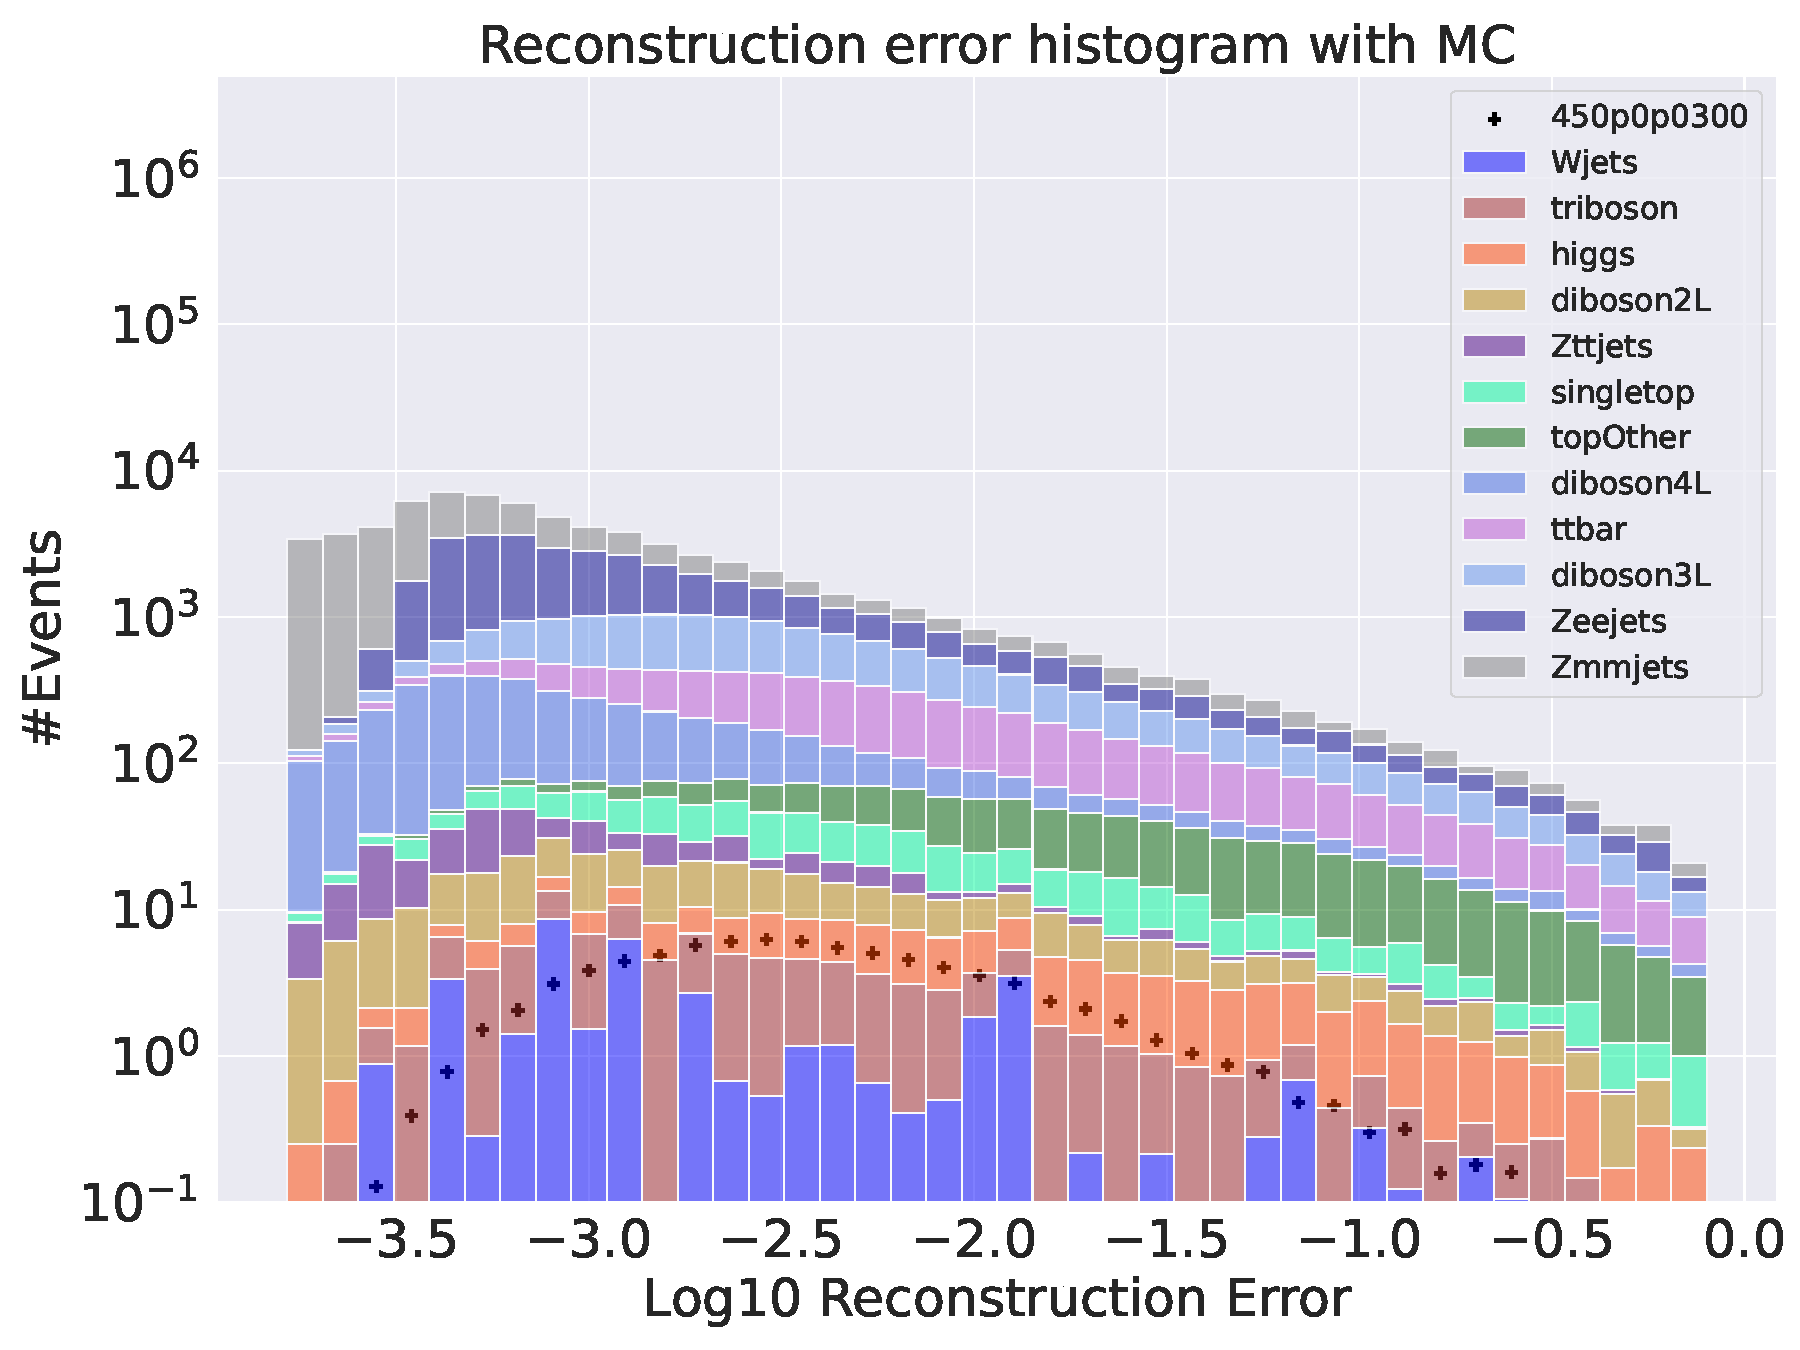
\includegraphics[width=\textwidth]{Figures/AE_testing/big/3lep/b_data_recon_big_rm3_feats_sig_450p0p0300.pdf}
        \caption{ }
        \label{fig:AE_3lep_big_450}
    \end{subfigure}
    \hfill
    \begin{subfigure}{.49\textwidth}
        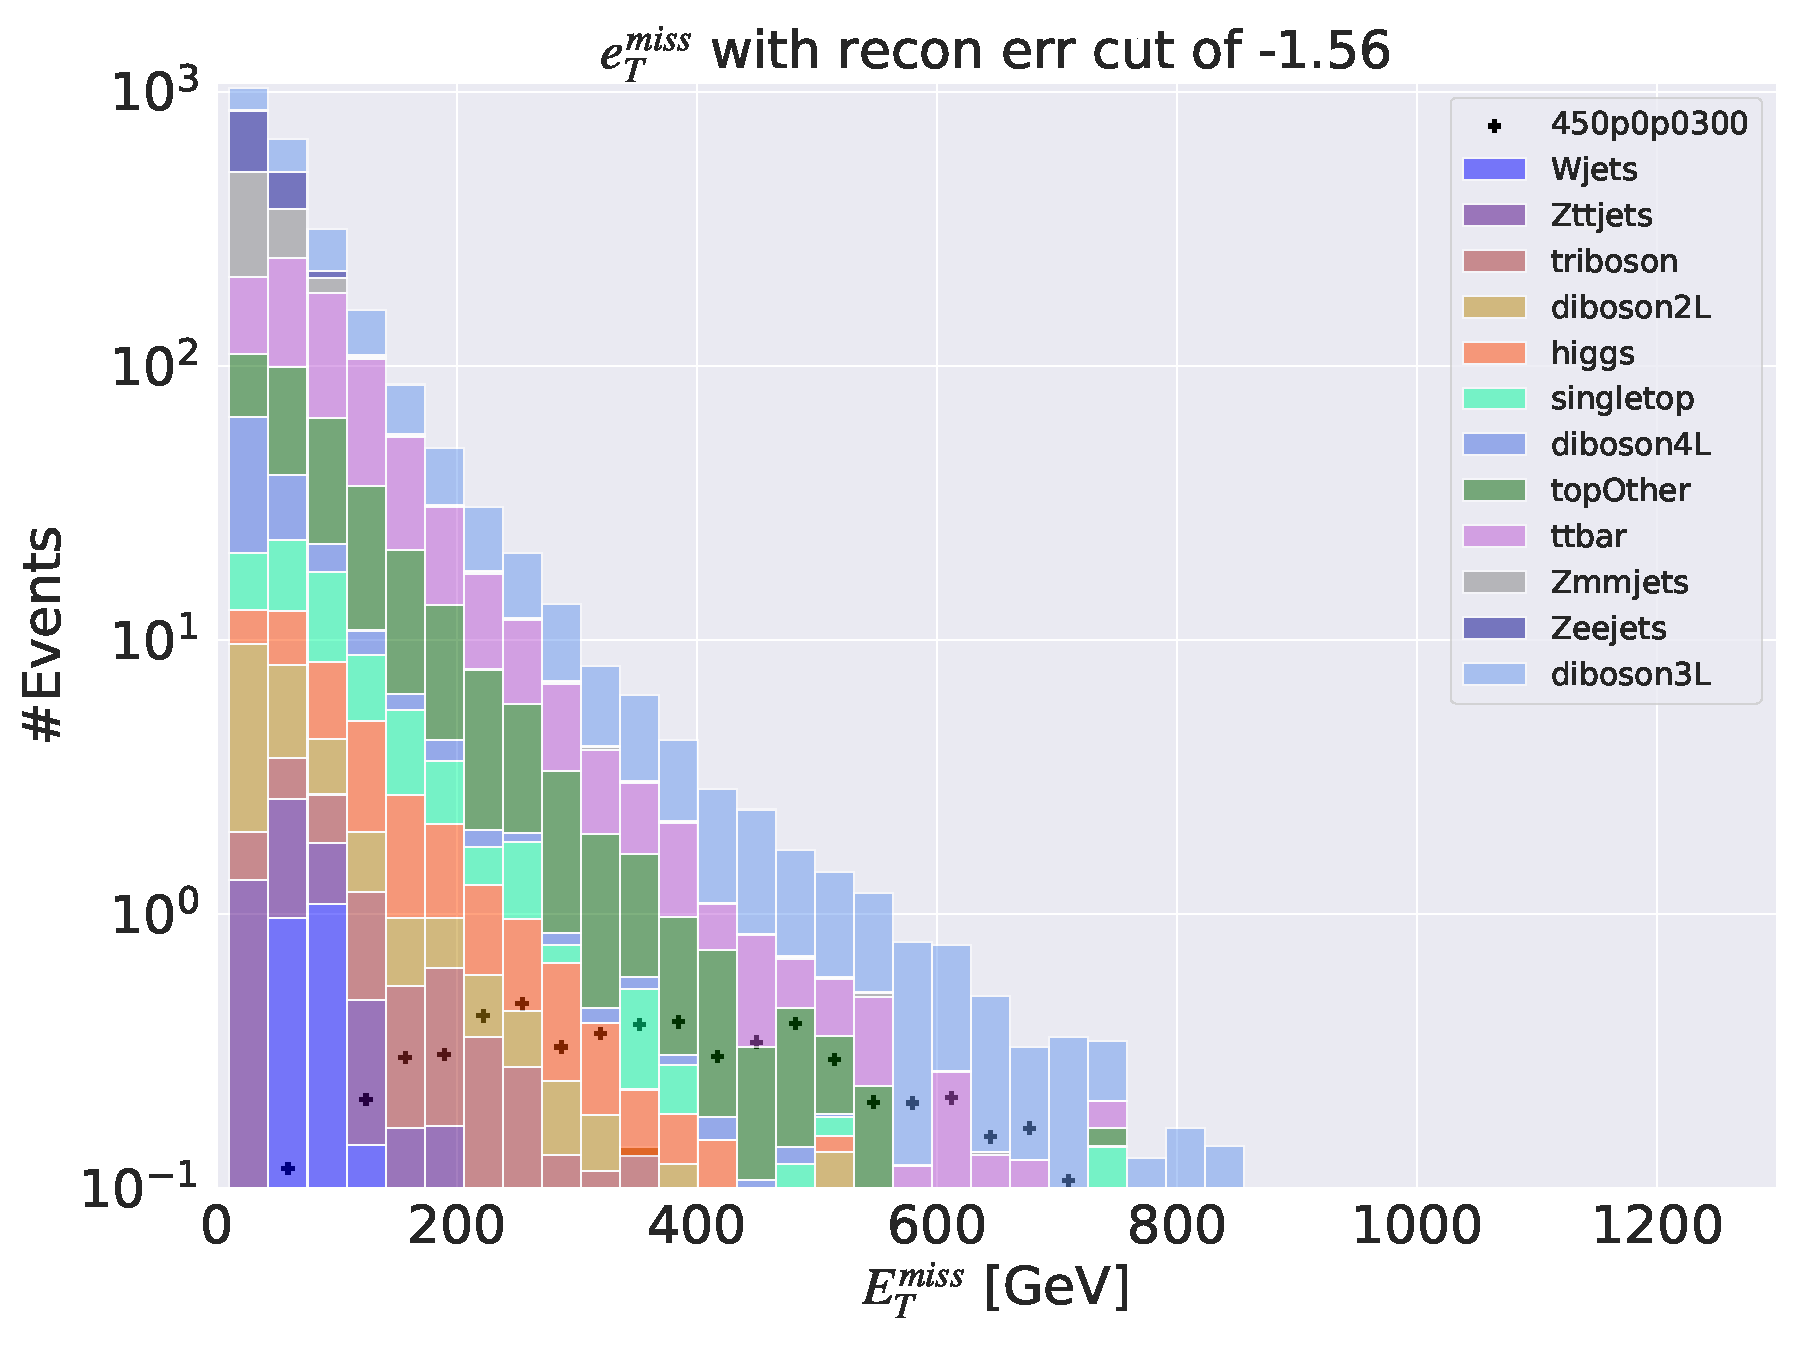
\includegraphics[width=\textwidth]{Figures/AE_testing/big/3lep/b_data_recon_big_rm3_feats_sig_450p0p0300_etmiss_recon_errcut_-1.56.pdf}
        \caption{}
        \label{fig:AE_3lep_big_etmiss_450}
    \end{subfigure}
    \hfill
    \begin{subfigure}{.49\textwidth}
        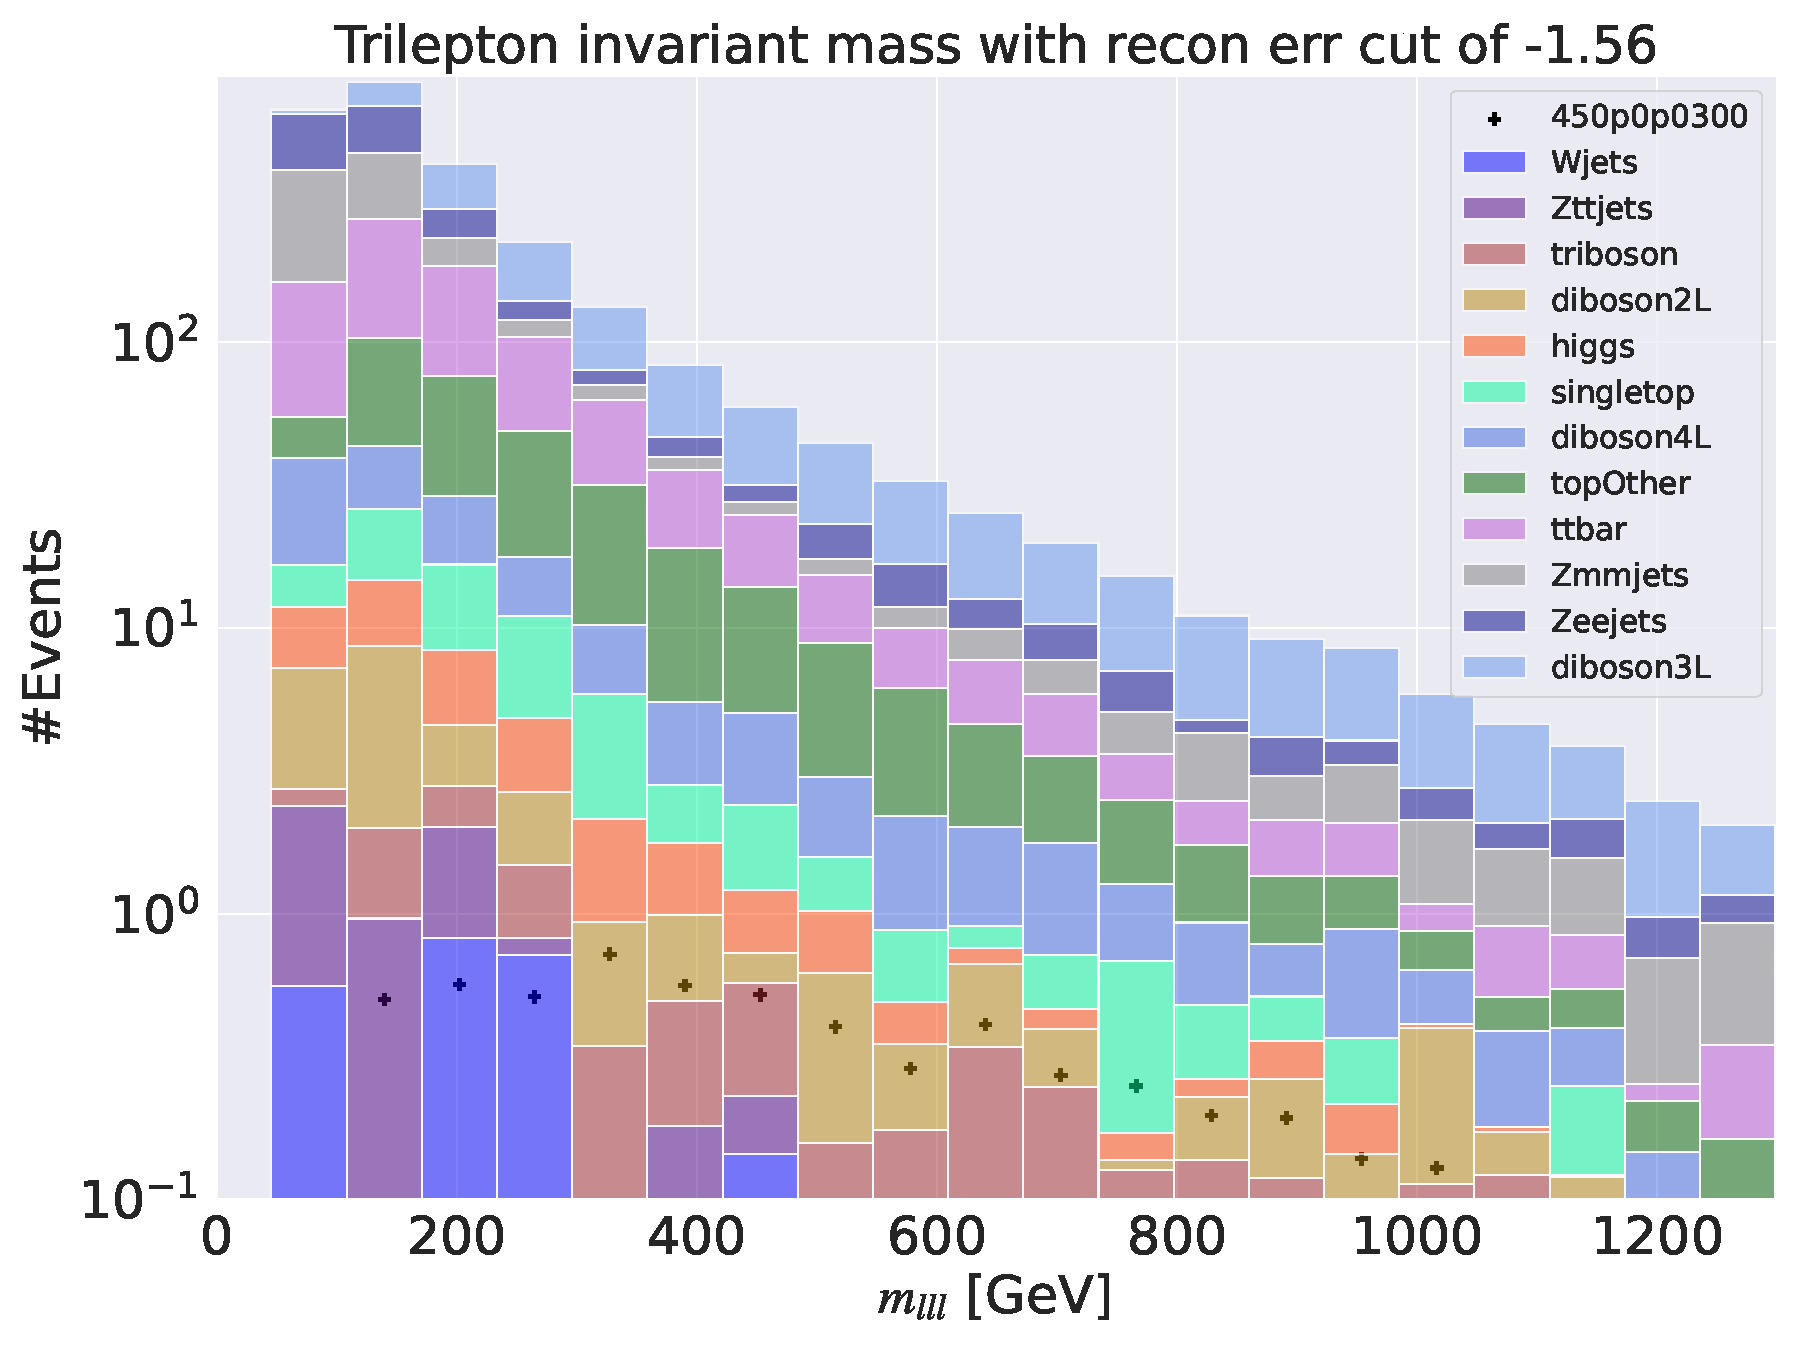
\includegraphics[width=\textwidth]{Figures/AE_testing/big/3lep/b_data_recon_big_rm3_feats_sig_450p0p0300_mlll_recon_errcut_-1.56.pdf}
        \caption{}
        \label{fig:AE_3lep_big_mlll_450}
    \end{subfigure}
    \hfill   
    \begin{subfigure}{.49\textwidth}
        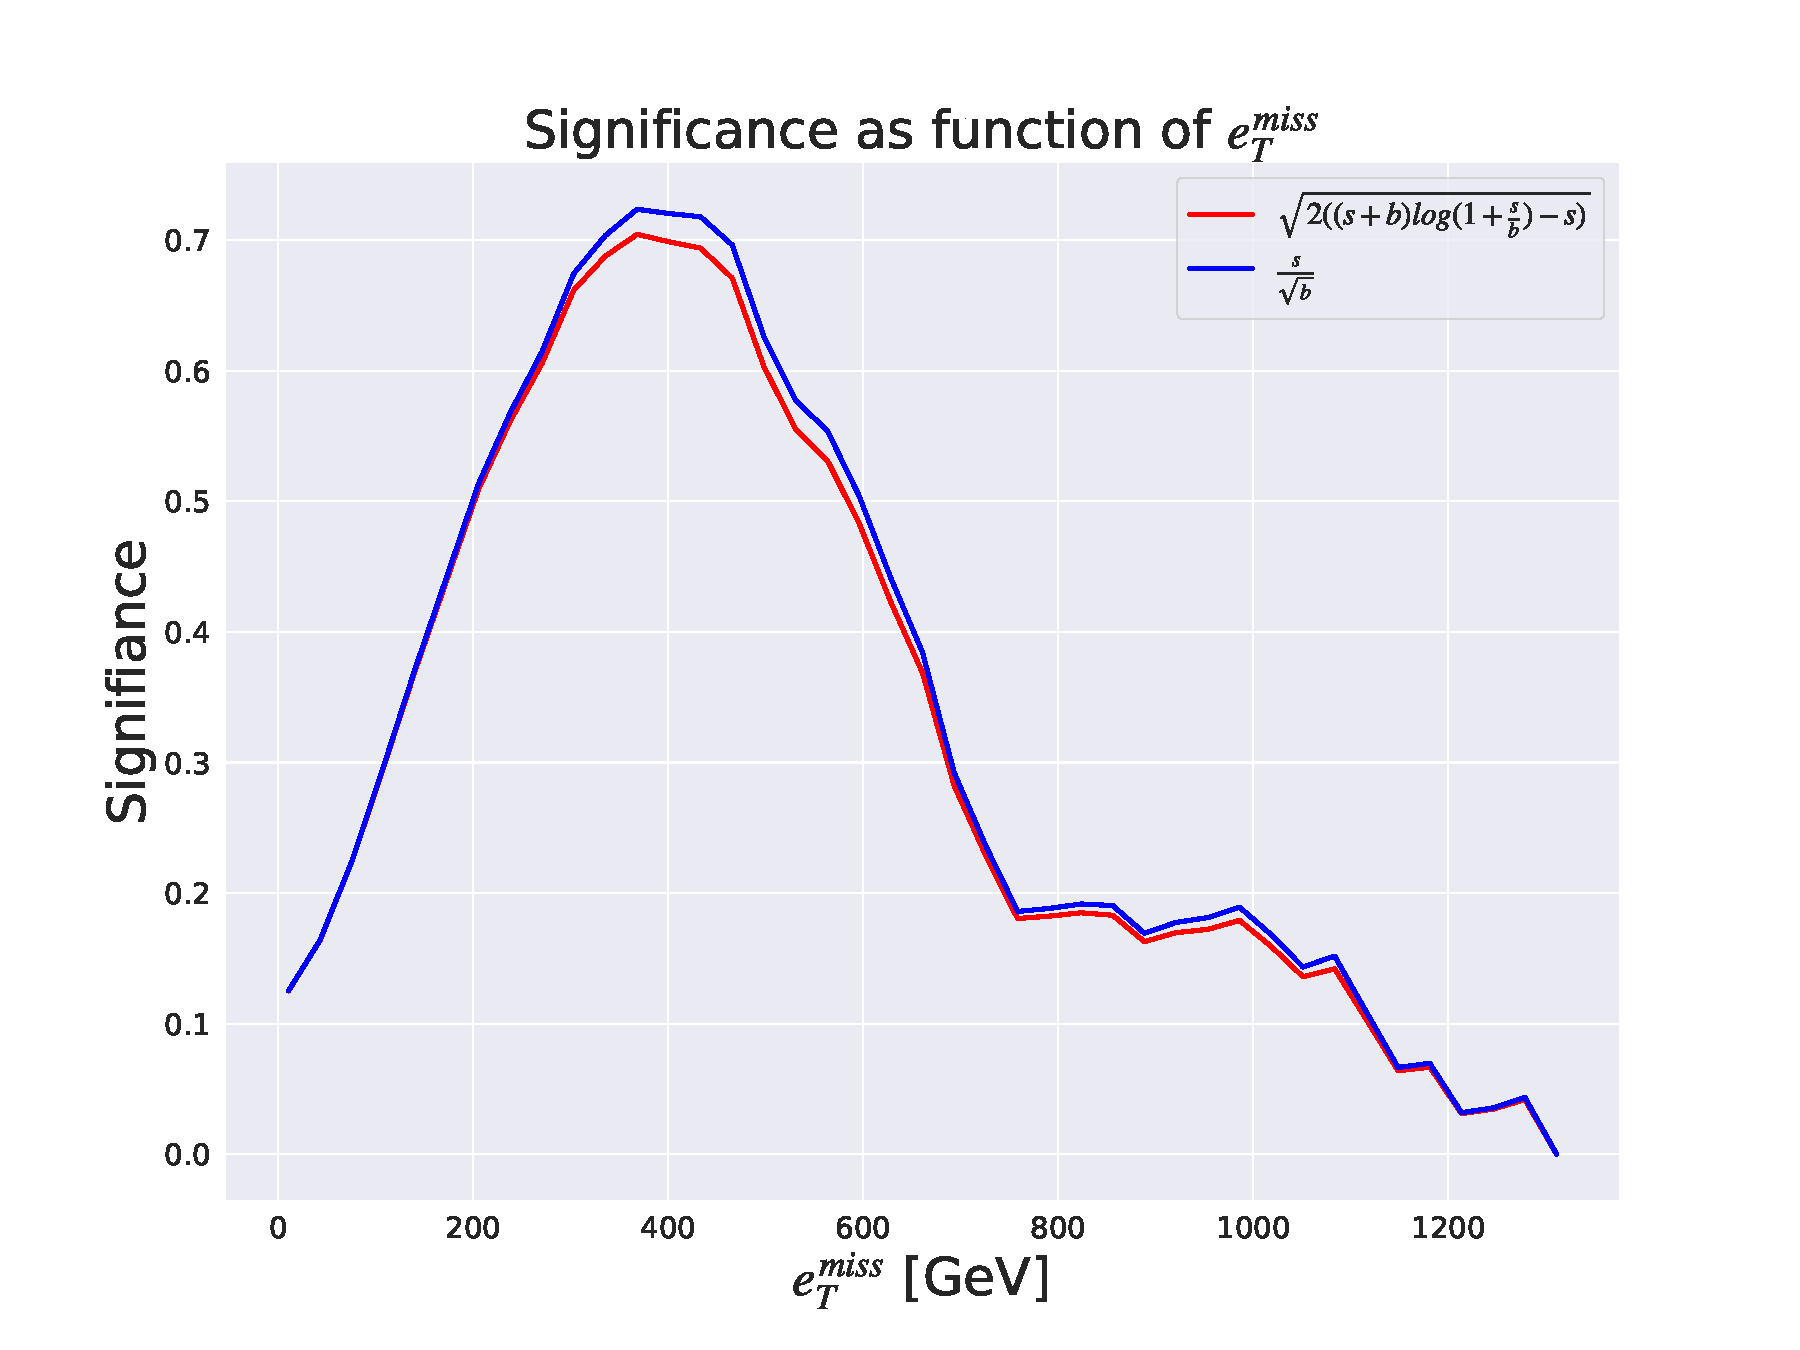
\includegraphics[width=\textwidth]{Figures/AE_testing/big/3lep/significance_etmiss_450p0p0300_-1.5648275418402864.pdf}
        \caption{}
        \label{fig:AE_3lep_big_signi_450}
    \end{subfigure}
    \hfill      
    \caption[3lep deep network | $450p300$ | AE]{Reconstruction error, $e_T^{miss}$ signal region, $m_{lll}$ signal region and significance as function of 
    $e_T^{miss}$ for the deep regular autoencoder using the SUSY $450p300$. Figure \ref{fig:AE_3lep_big_450} shows the reconstruction error 
    distribution for the SM MC and the SUSY signal. Here the autoencoder produces the same reconstruction error shape for both background and 
    signal. Figure \ref{fig:AE_3lep_big_etmiss_450} shows the $e_T^{miss}$ distribution for the SM MC and the SUSY signal in the signal region. 
    The signal region is made using a cut around $10^{-1.56}$. Most of the background is removed, and the peaks of the SM MC and signal 
    distributions are slightly separated. Figure \ref{fig:AE_3lep_big_mlll_450} shows the $m_{lll}$ distribution for the SM MC and the SUSY signal. 
    The shape of both distributions are too similar to distinguish. Figure \ref{fig:AE_3lep_big_signi_450} shows the significance as function of
    $e_T^{miss}$. The peak is put around a cut of about 380 GeV in the $e_T^{miss}$, with a significance of around $0.7$.}
    \label{fig:AE_3lep_big_rec_sig_signi_450}
\end{figure}

\begin{figure}[h!]
    \centering
    \begin{subfigure}{.49\textwidth}
        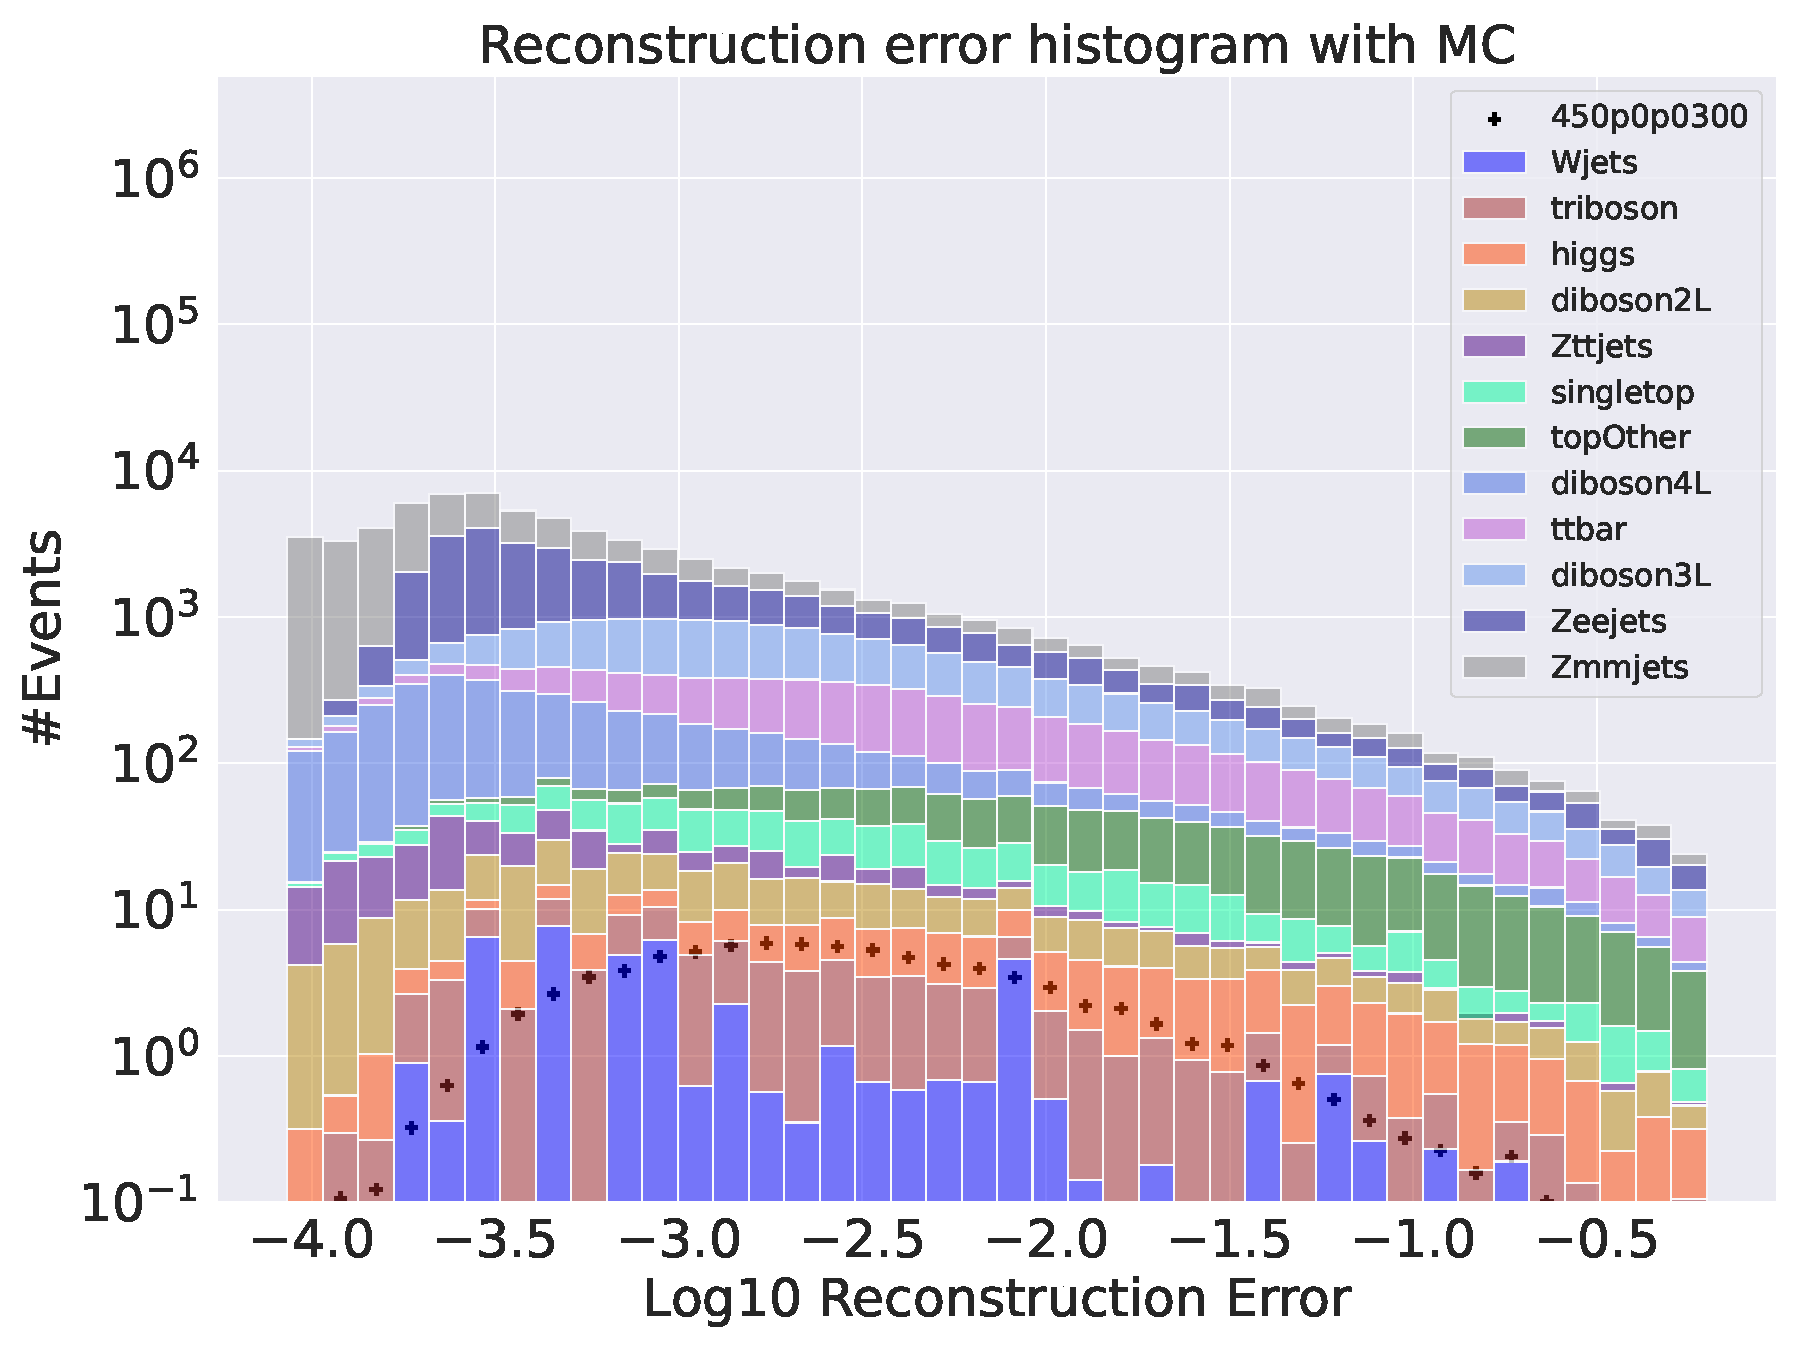
\includegraphics[width=\textwidth]{Figures/AE_testing/small/3lep/b_data_recon_big_rm3_feats_sig_450p0p0300.pdf}
        \caption{ }
        \label{fig:AE_3lep_small_450}
    \end{subfigure}
    \hfill
    \begin{subfigure}{.49\textwidth}
        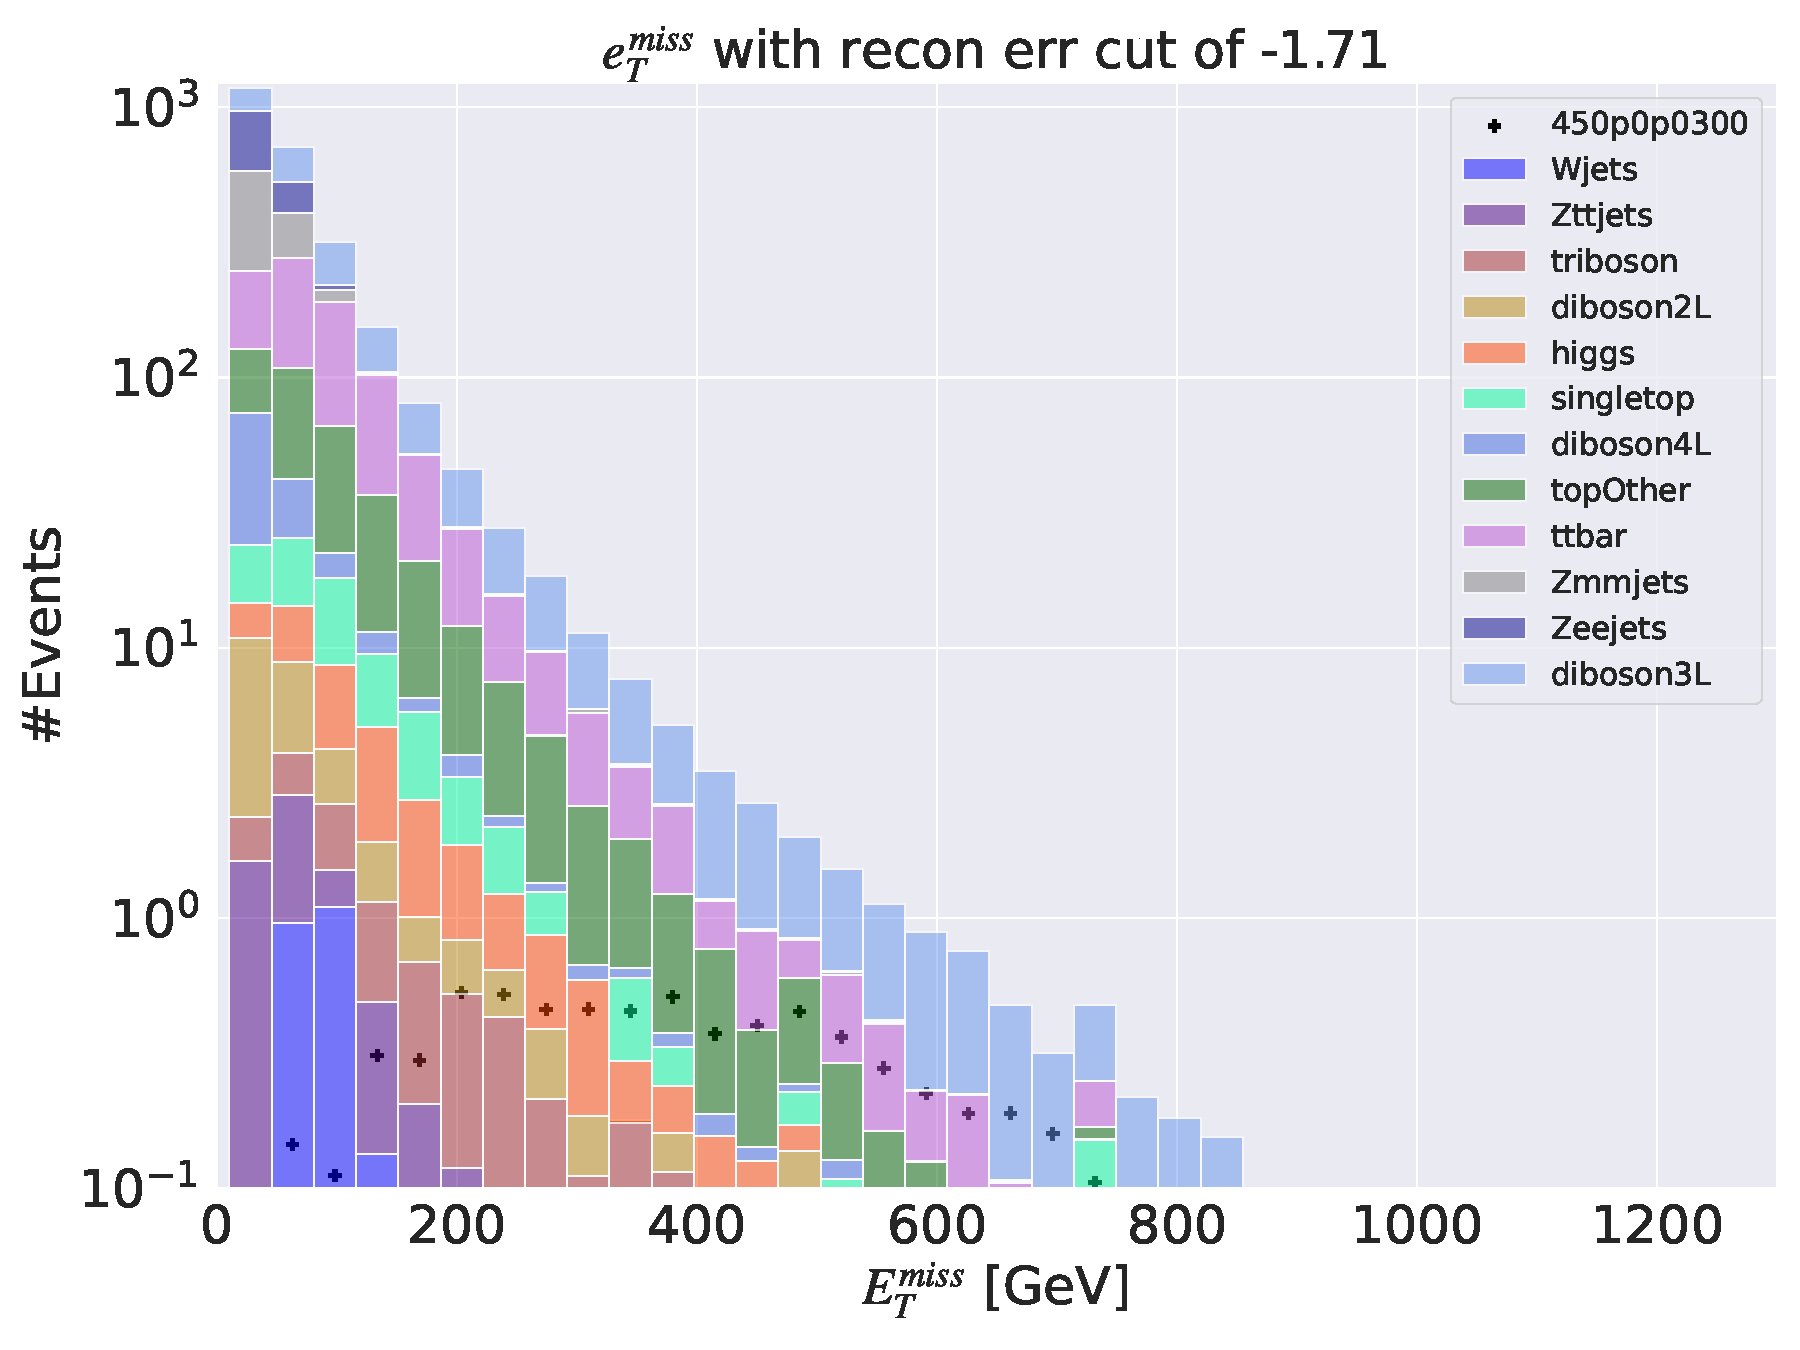
\includegraphics[width=\textwidth]{Figures/AE_testing/small/3lep/b_data_recon_big_rm3_feats_sig_450p0p0300_etmiss_recon_errcut_-1.71.pdf}
        \caption{}
        \label{fig:AE_3lep_small_etmiss_450}
    \end{subfigure}
    \hfill
    \begin{subfigure}{.49\textwidth}
        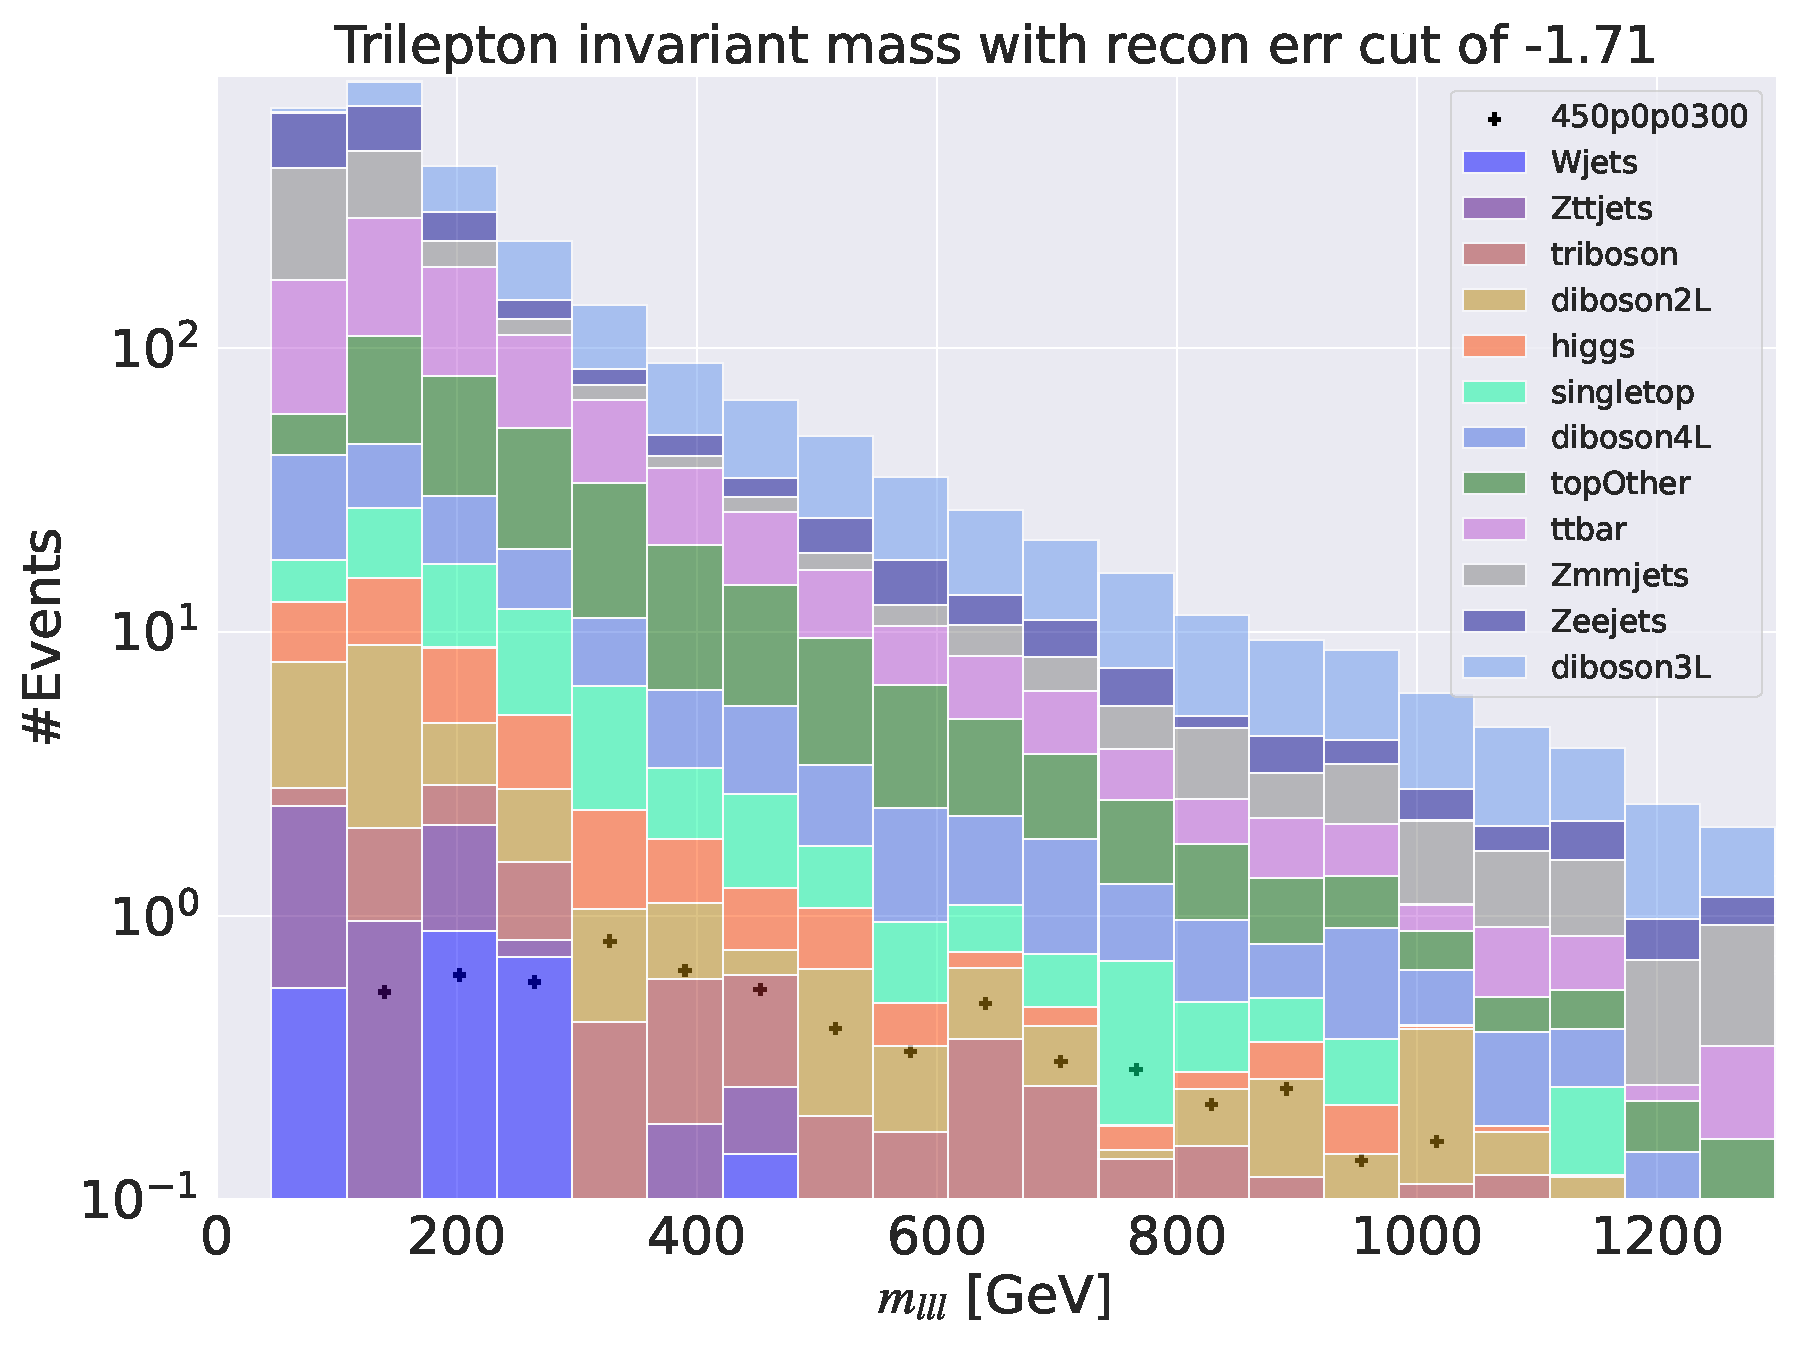
\includegraphics[width=\textwidth]{Figures/AE_testing/small/3lep/b_data_recon_big_rm3_feats_sig_450p0p0300_mlll_recon_errcut_-1.71.pdf}
        \caption{}
        \label{fig:AE_3lep_small_mlll_450}
    \end{subfigure}
    \hfill   
    \begin{subfigure}{.49\textwidth}
        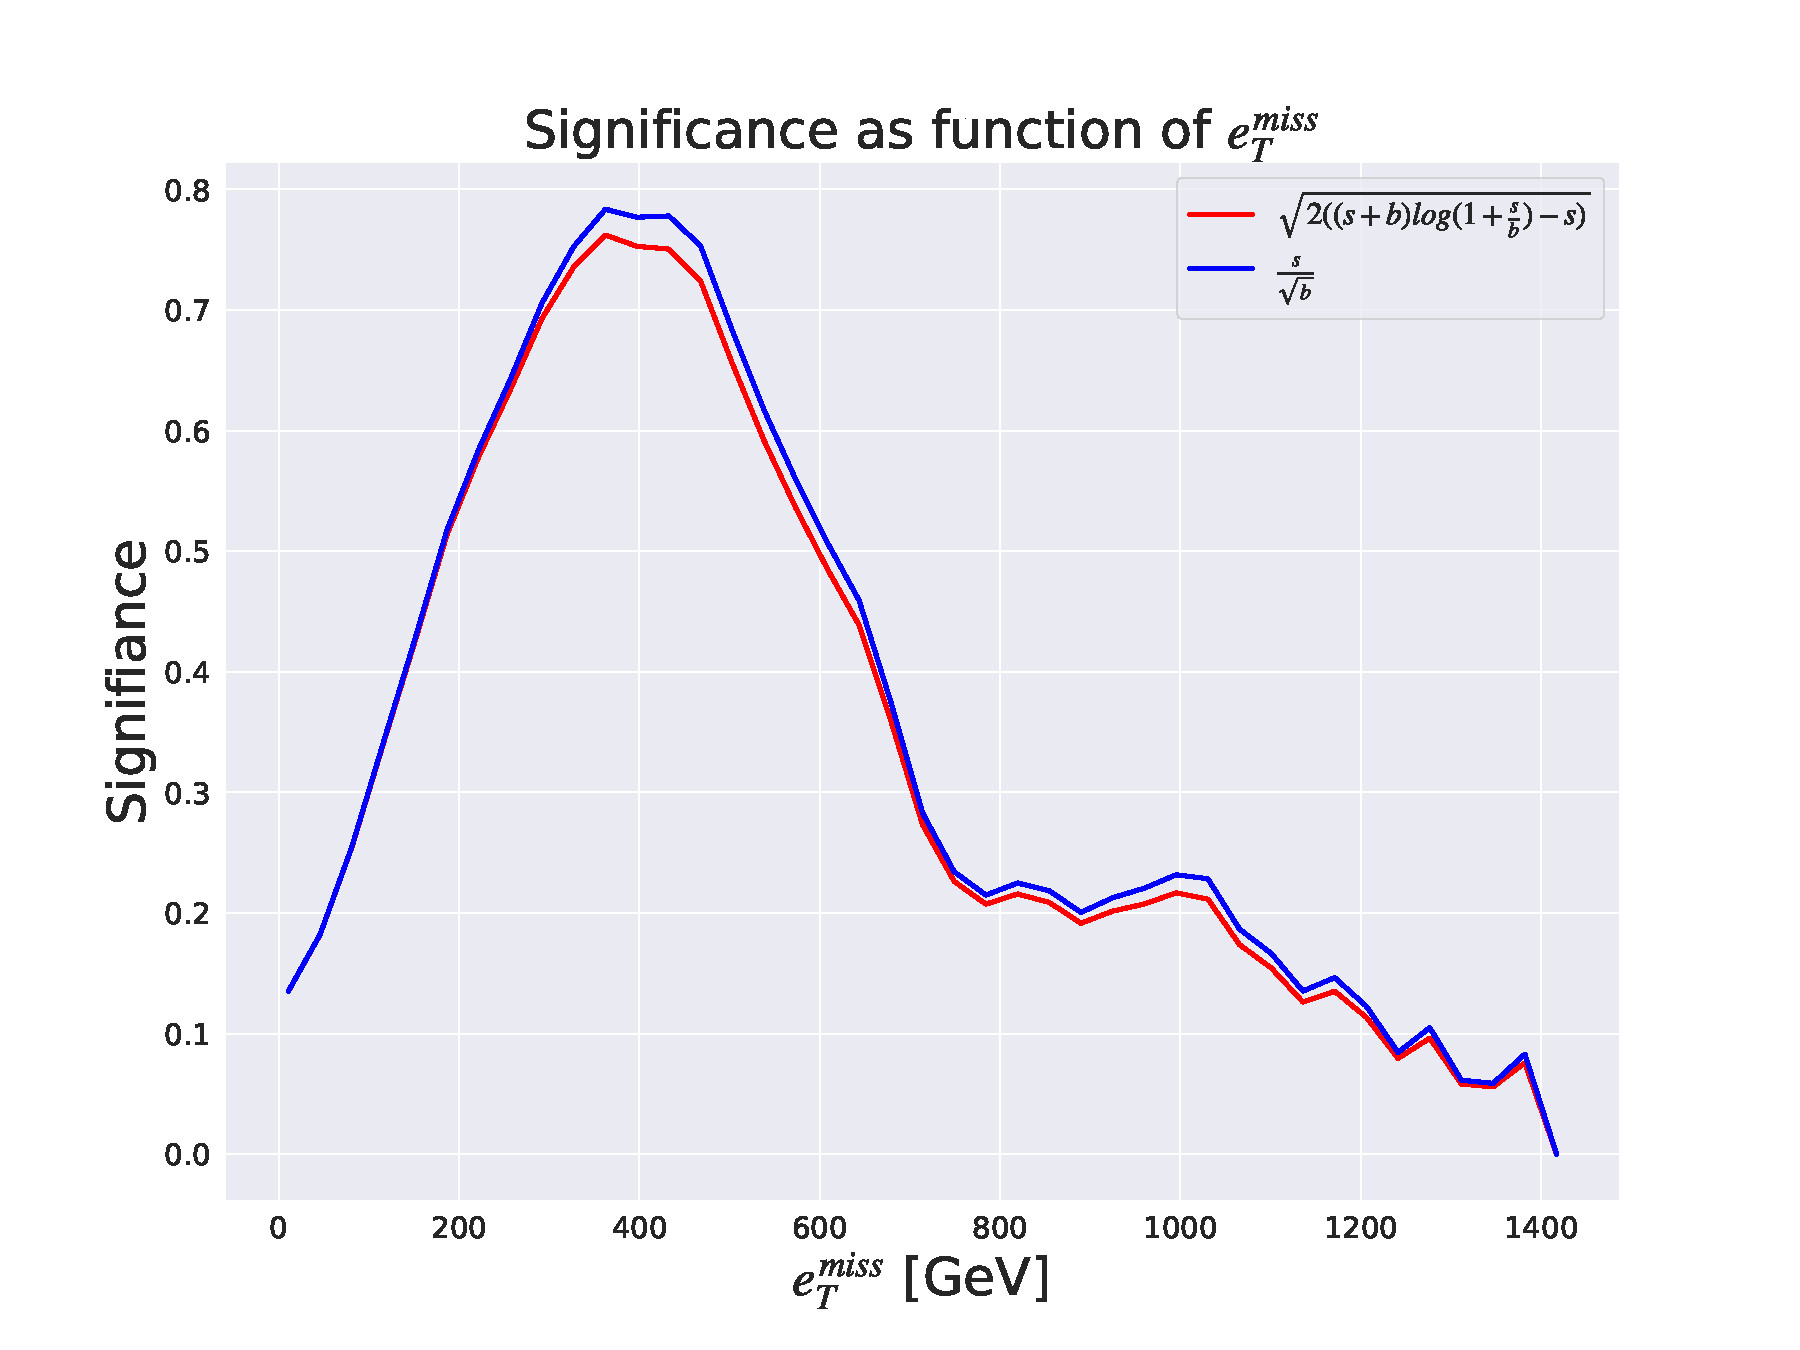
\includegraphics[width=\textwidth]{Figures/AE_testing/small/3lep/significance_etmiss_450p0p0300_-1.7067960296617328.pdf}
        \caption{}
        \label{fig:AE_3lep_small_signi_450}
    \end{subfigure}
    \hfill      
    \caption[3lep shallow network | $450p300$ | AE]{Reconstruction error, $e_T^{miss}$ signal region, $m_{lll}$ signal region and significance as function of 
    $e_T^{miss}$ for the shallow regular autoencoder using the SUSY $450p300$ model. Figure \ref{fig:AE_3lep_small_450} shows the reconstruction error 
    distribution for the SM MC and the SUSY signal. Here the autoencoder produces the same reconstruction error shape for both background and 
    signal, but with a small separation of the peaks of the distributions. Figure \ref{fig:AE_3lep_small_etmiss_450} shows the $e_T^{miss}$ 
    distribution for the SM MC and the SUSY signal in the signal region. The signal region is made using a cut around $10^{-1.71}$. Most of 
    the background is removed, and the peaks of the SM MC and signal distributions are somewhat separated. Figure 
    \ref{fig:AE_3lep_small_mlll_450} shows the $m_{lll}$ distribution for the SM MC and the SUSY signal. 
    The shape of both distributions are too similar to distinguish. Figure \ref{fig:AE_3lep_small_signi_450} shows the significance as 
    function of $e_T^{miss}$. The peak is put around a cut of about 380 GeV in the $e_T^{miss}$, with a significance of around $0.78$.}
    \label{fig:AE_3lep_small_rec_sig_signi_450}
\end{figure}








\begin{figure}[h!]
    \centering
    \begin{subfigure}{.49\textwidth}
        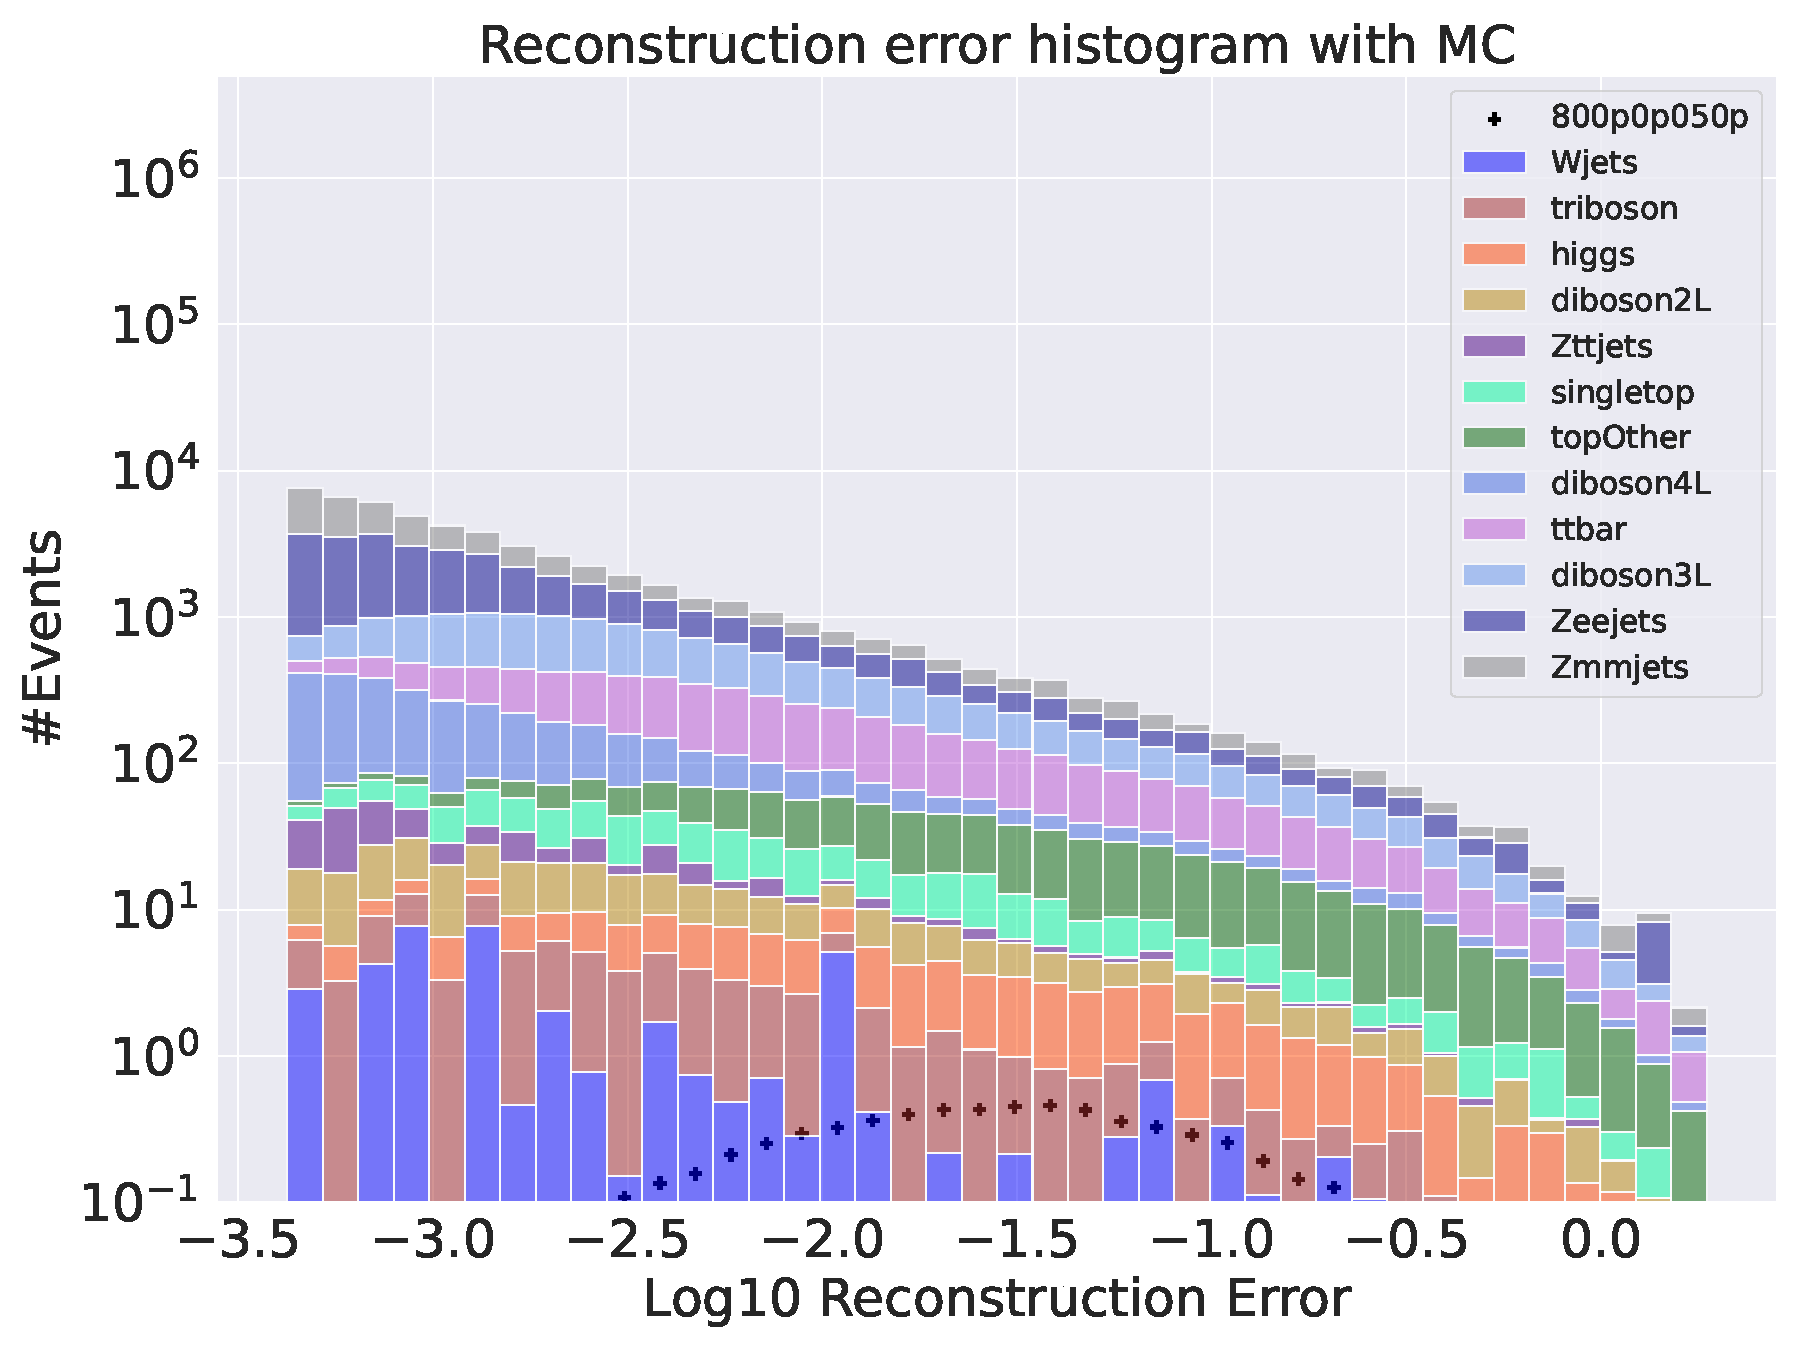
\includegraphics[width=\textwidth]{Figures/AE_testing/big/3lep/b_data_recon_big_rm3_feats_sig_800p0p050p.pdf}
        \caption{ }
        \label{fig:AE_3lep_big_800}
    \end{subfigure}
    \hfill
    \begin{subfigure}{.49\textwidth}
        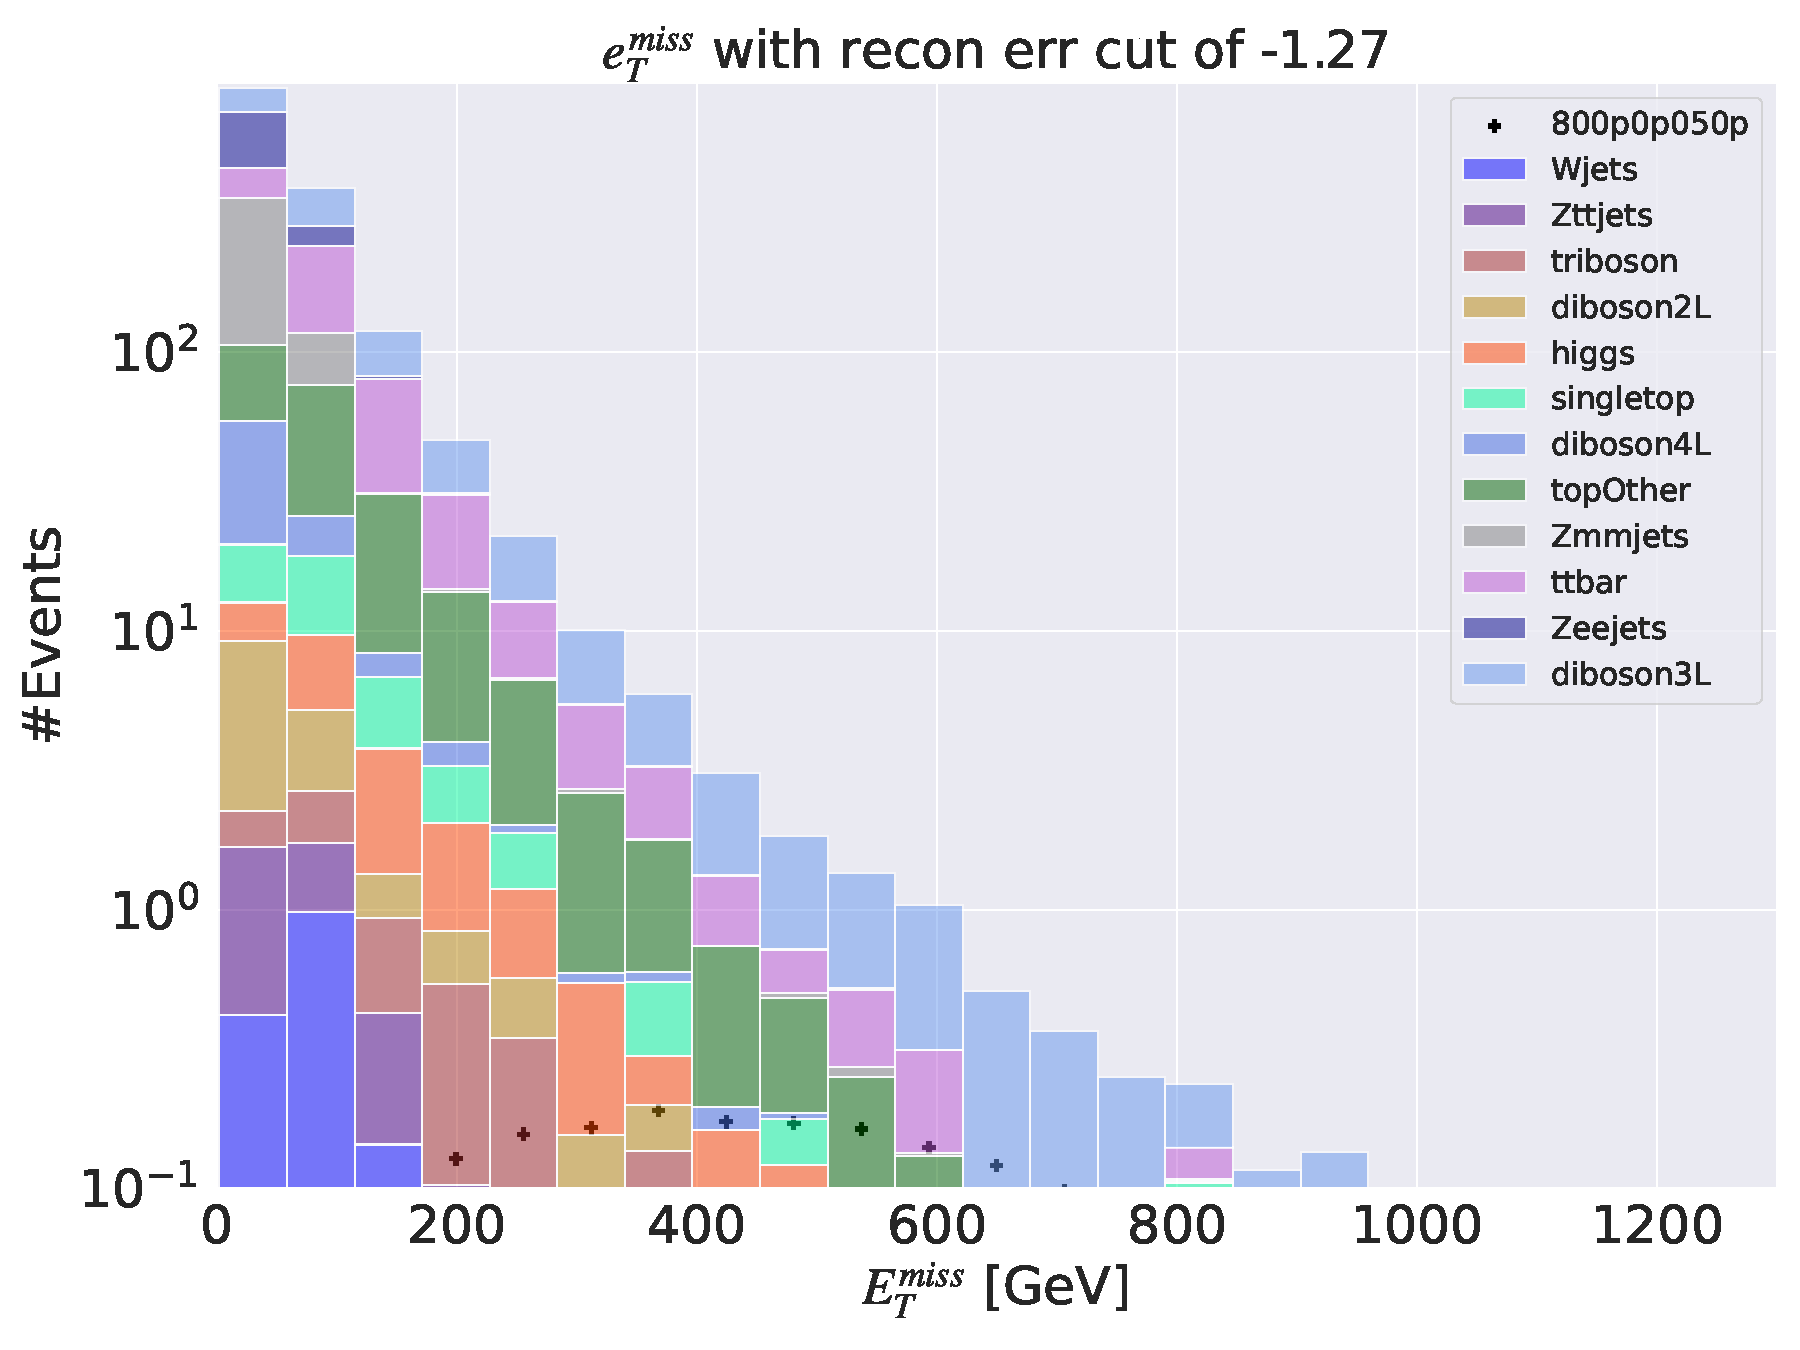
\includegraphics[width=\textwidth]{Figures/AE_testing/big/3lep/b_data_recon_big_rm3_feats_sig_800p0p050p_etmiss_recon_errcut_-1.27.pdf}
        \caption{}
        \label{fig:AE_3lep_big_etmiss_800}
    \end{subfigure}
    \hfill
    \begin{subfigure}{.49\textwidth}
        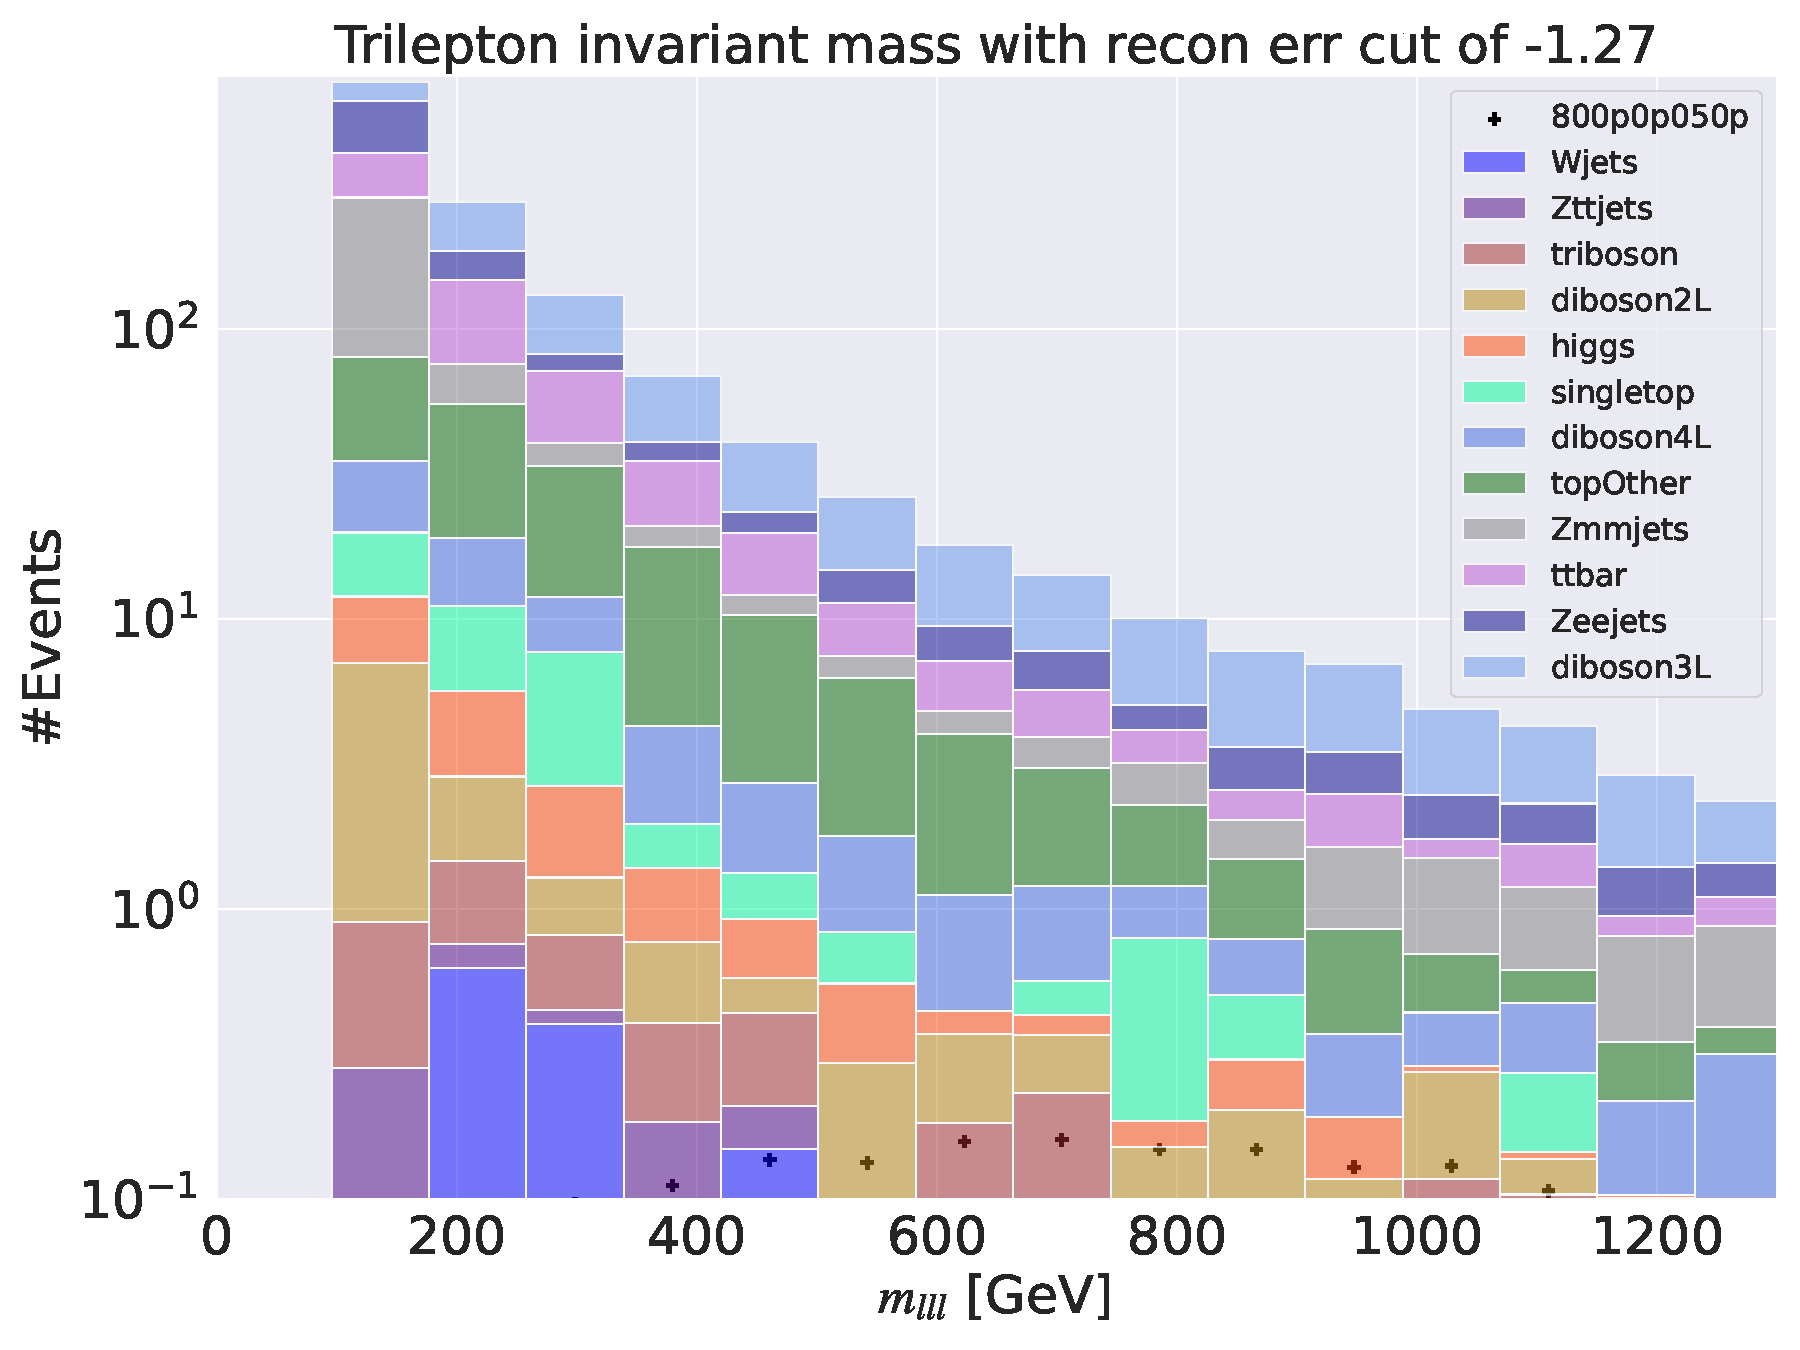
\includegraphics[width=\textwidth]{Figures/AE_testing/big/3lep/b_data_recon_big_rm3_feats_sig_800p0p050p_mlll_recon_errcut_-1.27.pdf}
        \caption{}
        \label{fig:AE_3lep_big_mlll_800}
    \end{subfigure}
    \hfill   
    \begin{subfigure}{.49\textwidth}
        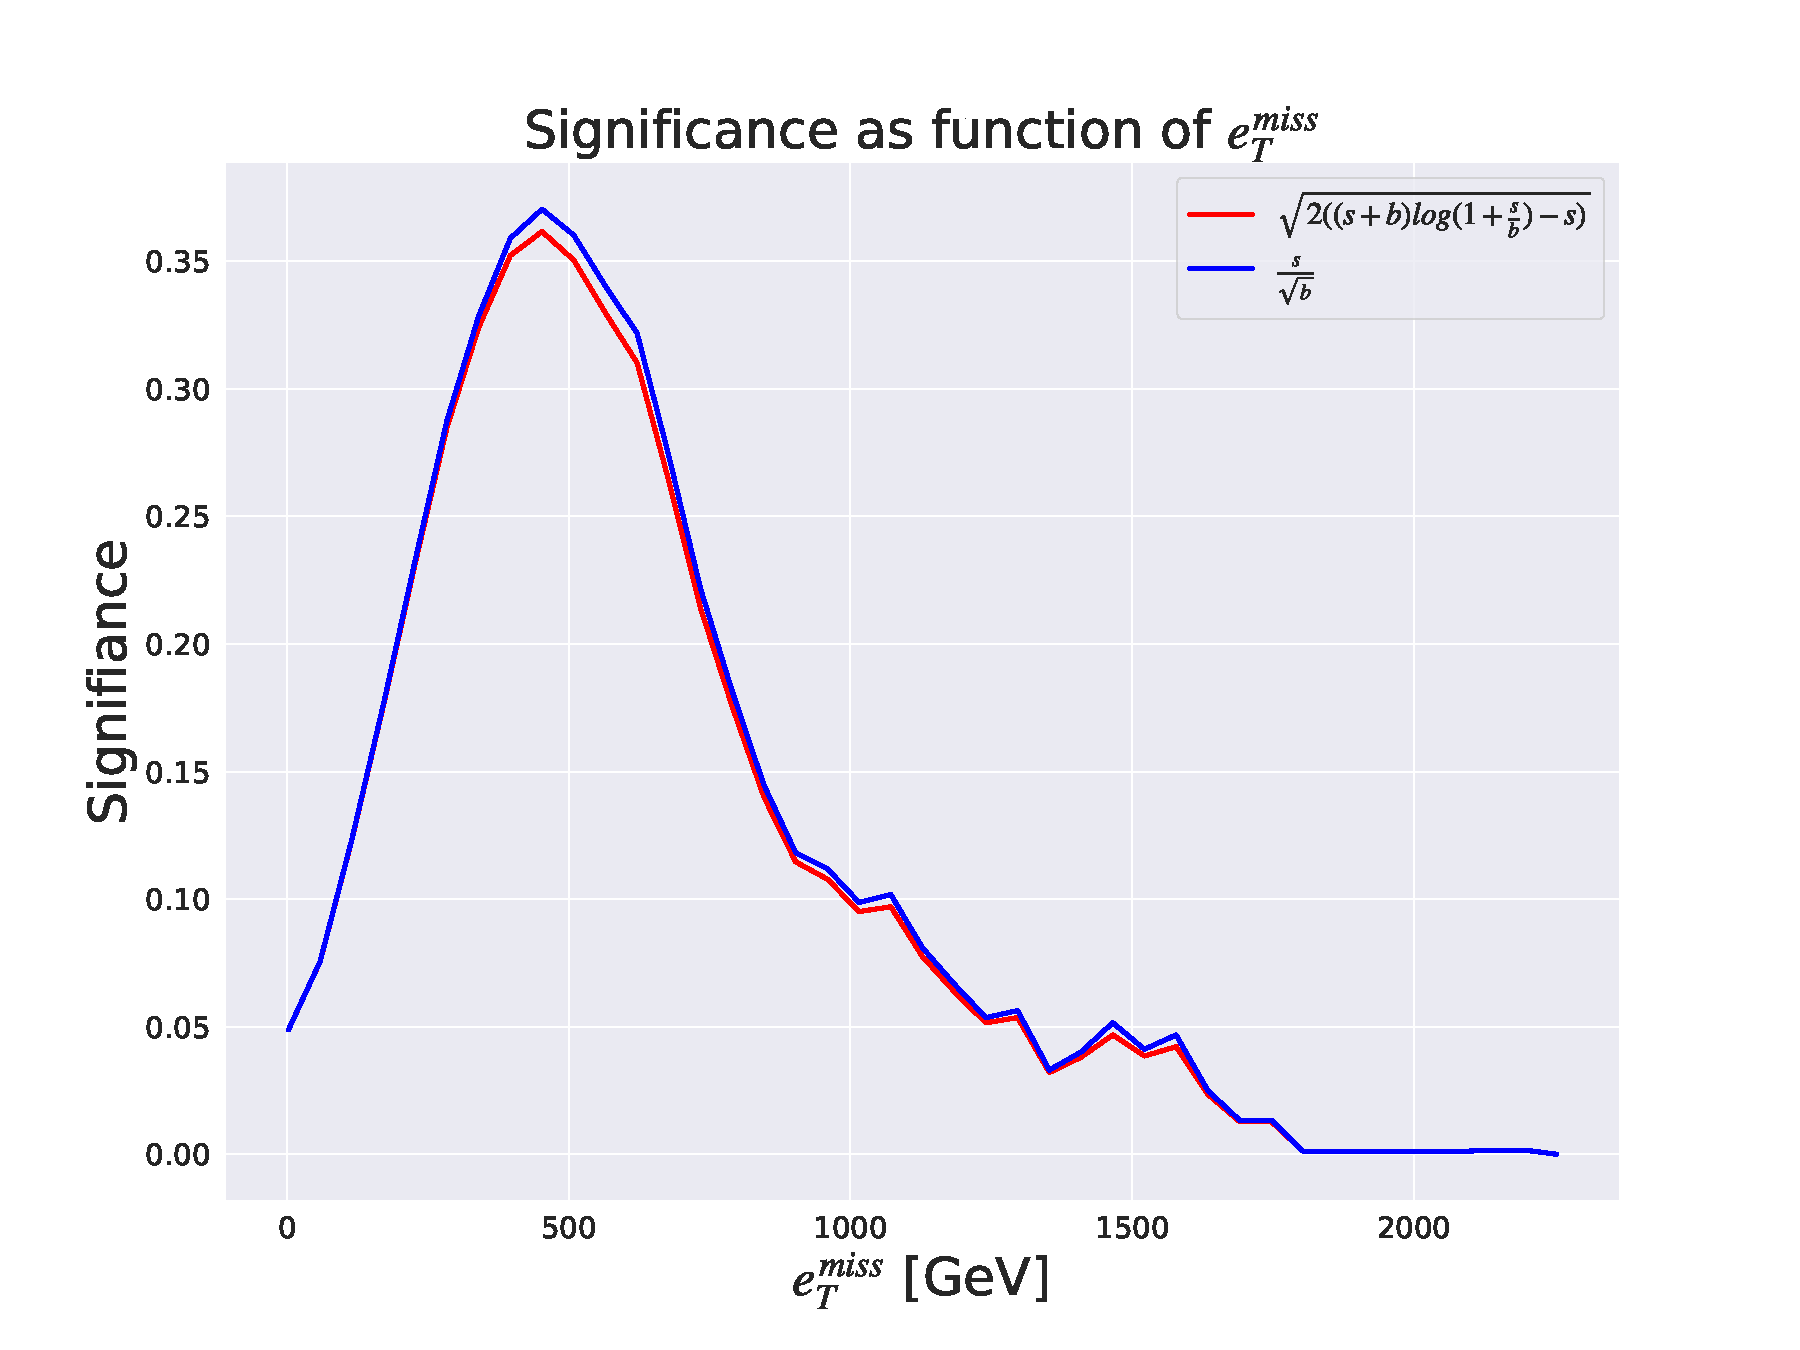
\includegraphics[width=\textwidth]{Figures/AE_testing/big/3lep/significance_etmiss_800p0p050p_-1.2726592563014343.pdf}
        \caption{}
        \label{fig:AE_3lep_big_signi_800}
    \end{subfigure}
    \hfill      
    \caption[3lep deep network | $800p50$ | AE]{Reconstruction error, $e_T^{miss}$ signal region, $m_{lll}$ signal region and significance as function of 
    $e_T^{miss}$ for the deep regular autoencoder using the SUSY $800p50$. 
    Figure \ref{fig:AE_3lep_big_800} shows the reconstruction error 
    distribution for the SM MC and the SUSY signal. Here the autoencoder produces a mirrored reconstruction error shape for background and 
    signal. The peaks of the two distributions are separated with two orders of magnitude in reconstruction error. Figure \ref{fig:AE_3lep_big_etmiss_800} 
    shows the $e_T^{miss}$ distribution for the SM MC and the SUSY signal in the signal region. 
    The signal region is made using a cut around $10^{-1.27}$. Most of the background is removed, and the peaks of the SM MC and signal 
    distributions are separated. Figure \ref{fig:AE_3lep_big_mlll_800} shows the $m_{lll}$ distribution for the SM MC and the SUSY signal. 
    The shape of both distributions are somewhat separated. Figure \ref{fig:AE_3lep_big_signi_800} shows the significance as function of
    $e_T^{miss}$. The peak is put around a cut of about 430 GeV in the $e_T^{miss}$, with a significance of around $0.37$.}
    \label{fig:AE_3lep_big_rec_sig_signi_800}
\end{figure}

\begin{figure}[h!]
    \centering
    \begin{subfigure}{.49\textwidth}
        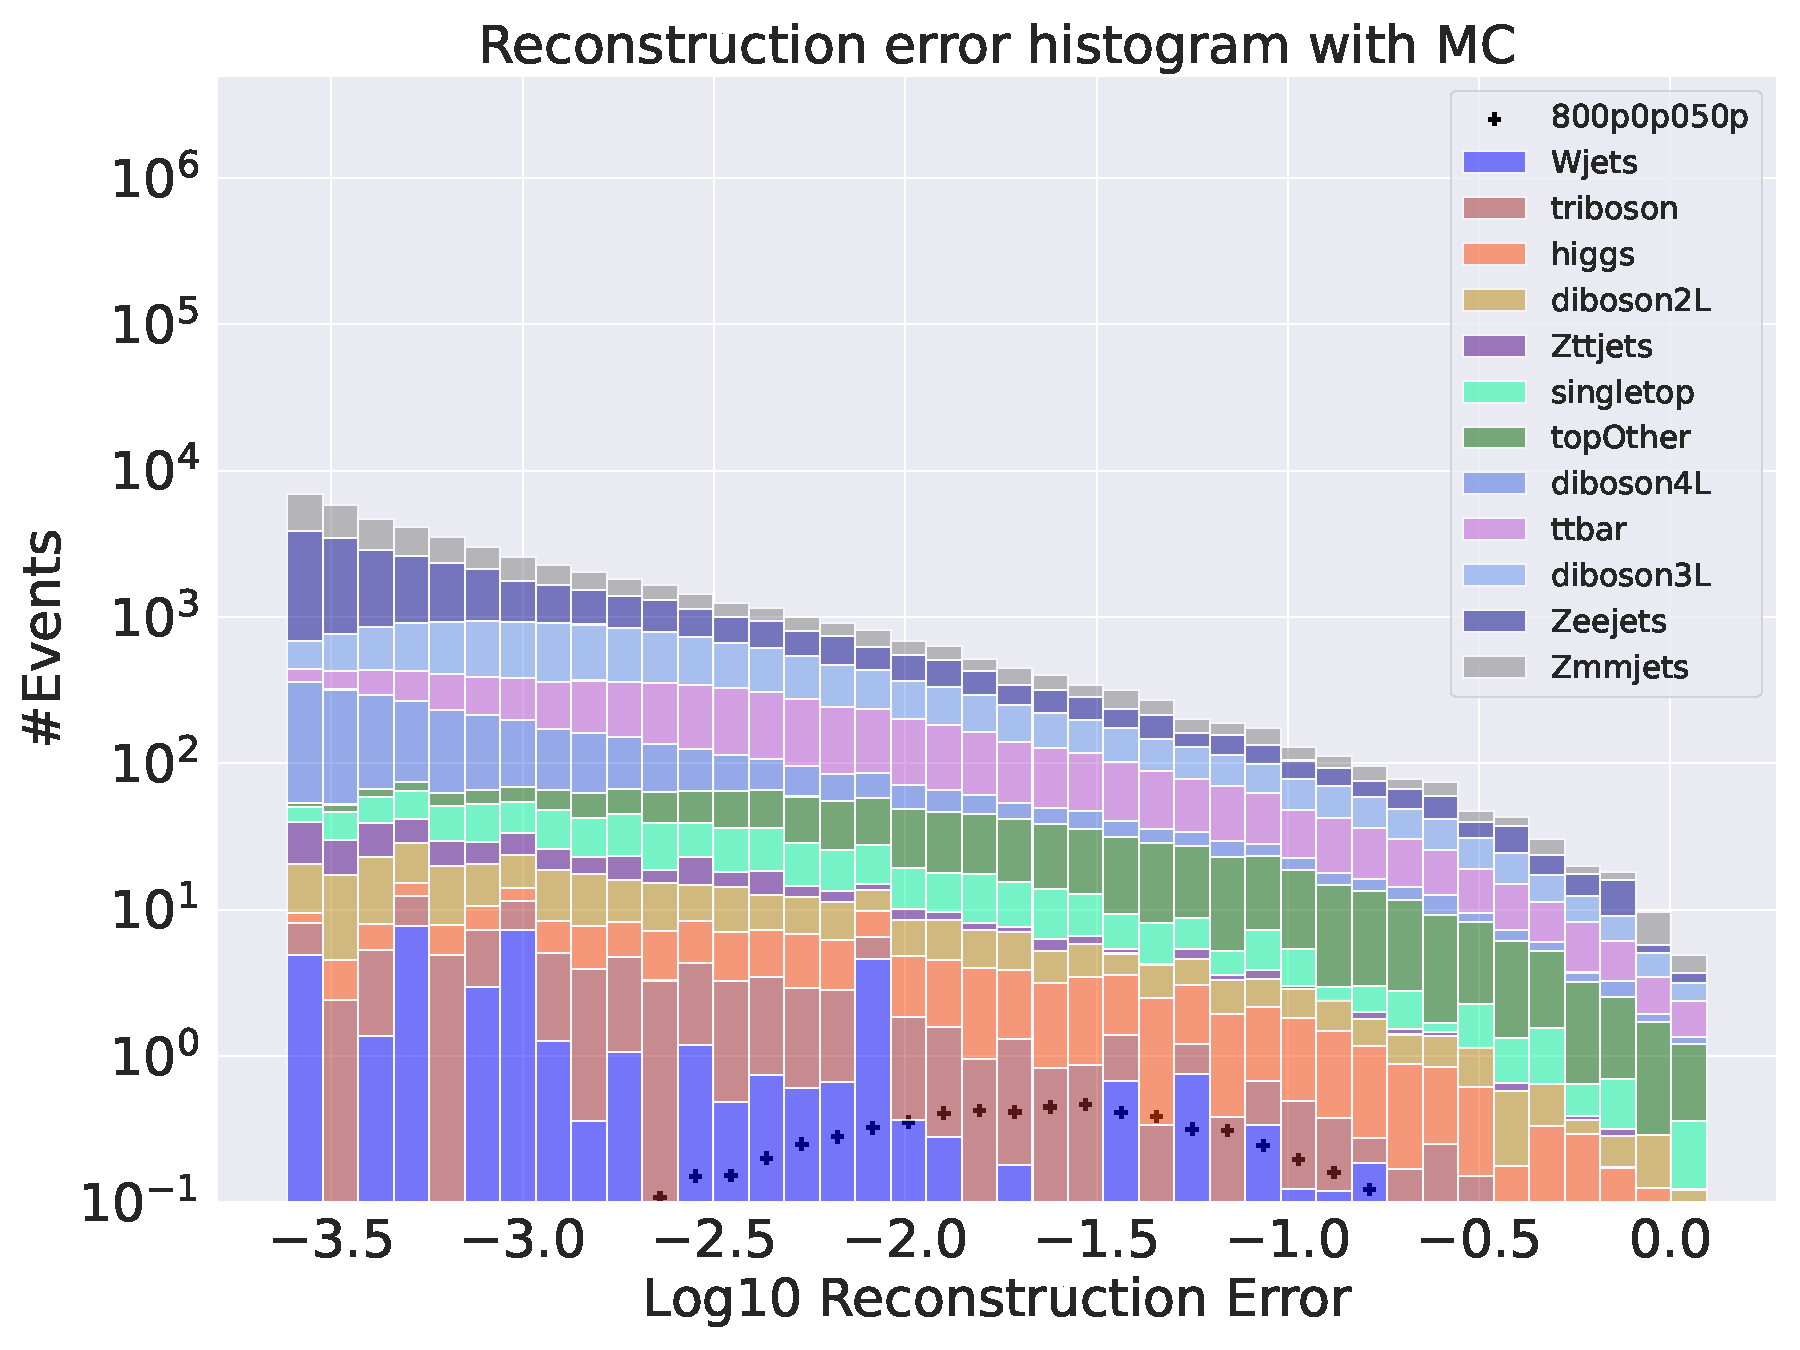
\includegraphics[width=\textwidth]{Figures/AE_testing/small/3lep/b_data_recon_big_rm3_feats_sig_800p0p050p.pdf}
        \caption{ }
        \label{fig:AE_3lep_small_800}
    \end{subfigure}
    \hfill
    \begin{subfigure}{.49\textwidth}
        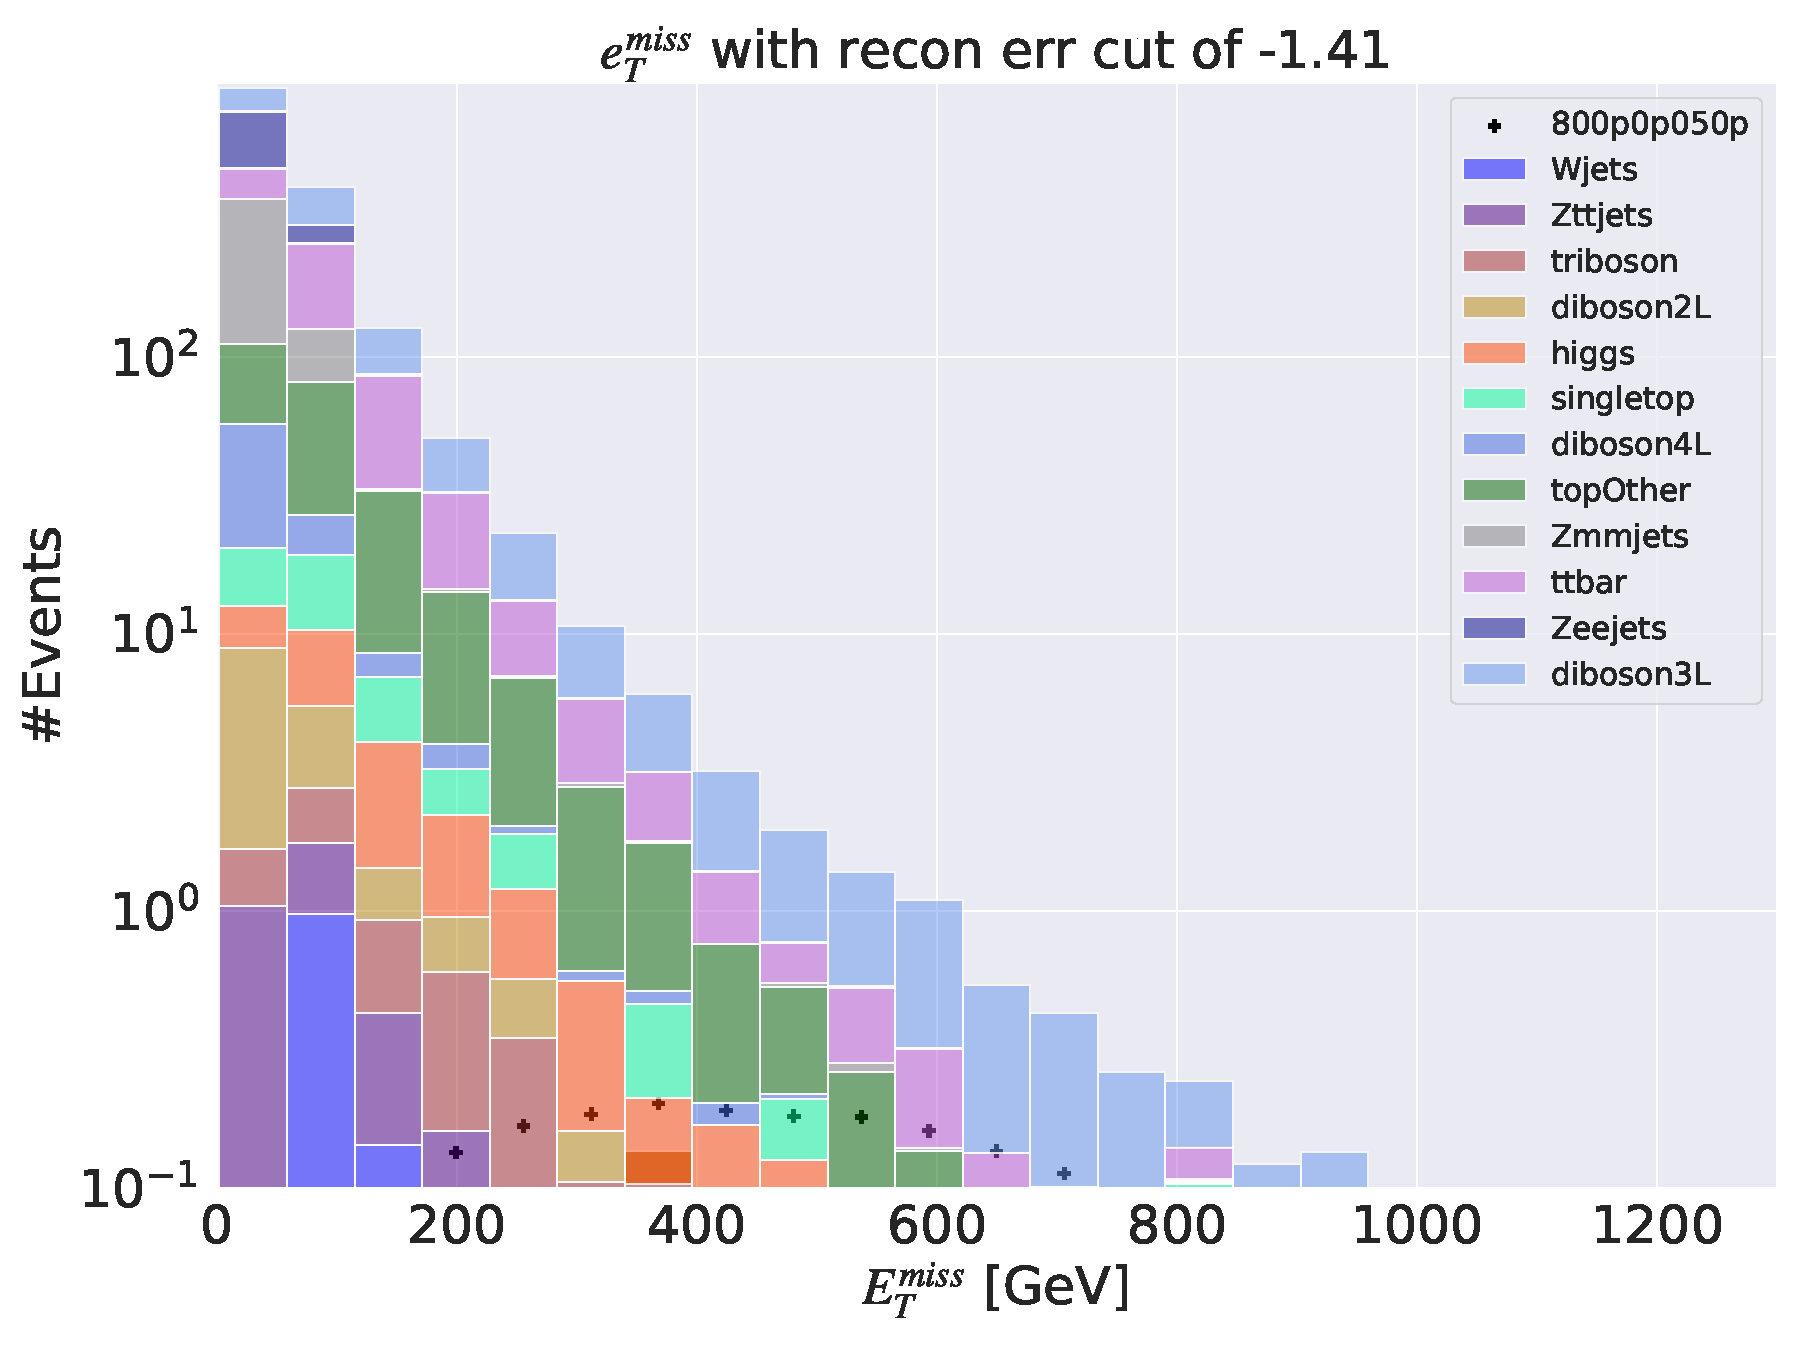
\includegraphics[width=\textwidth]{Figures/AE_testing/small/3lep/b_data_recon_big_rm3_feats_sig_800p0p050p_etmiss_recon_errcut_-1.41.pdf}
        \caption{}
        \label{fig:AE_3lep_small_etmiss_800}
    \end{subfigure}
    \hfill
    \begin{subfigure}{.49\textwidth}
        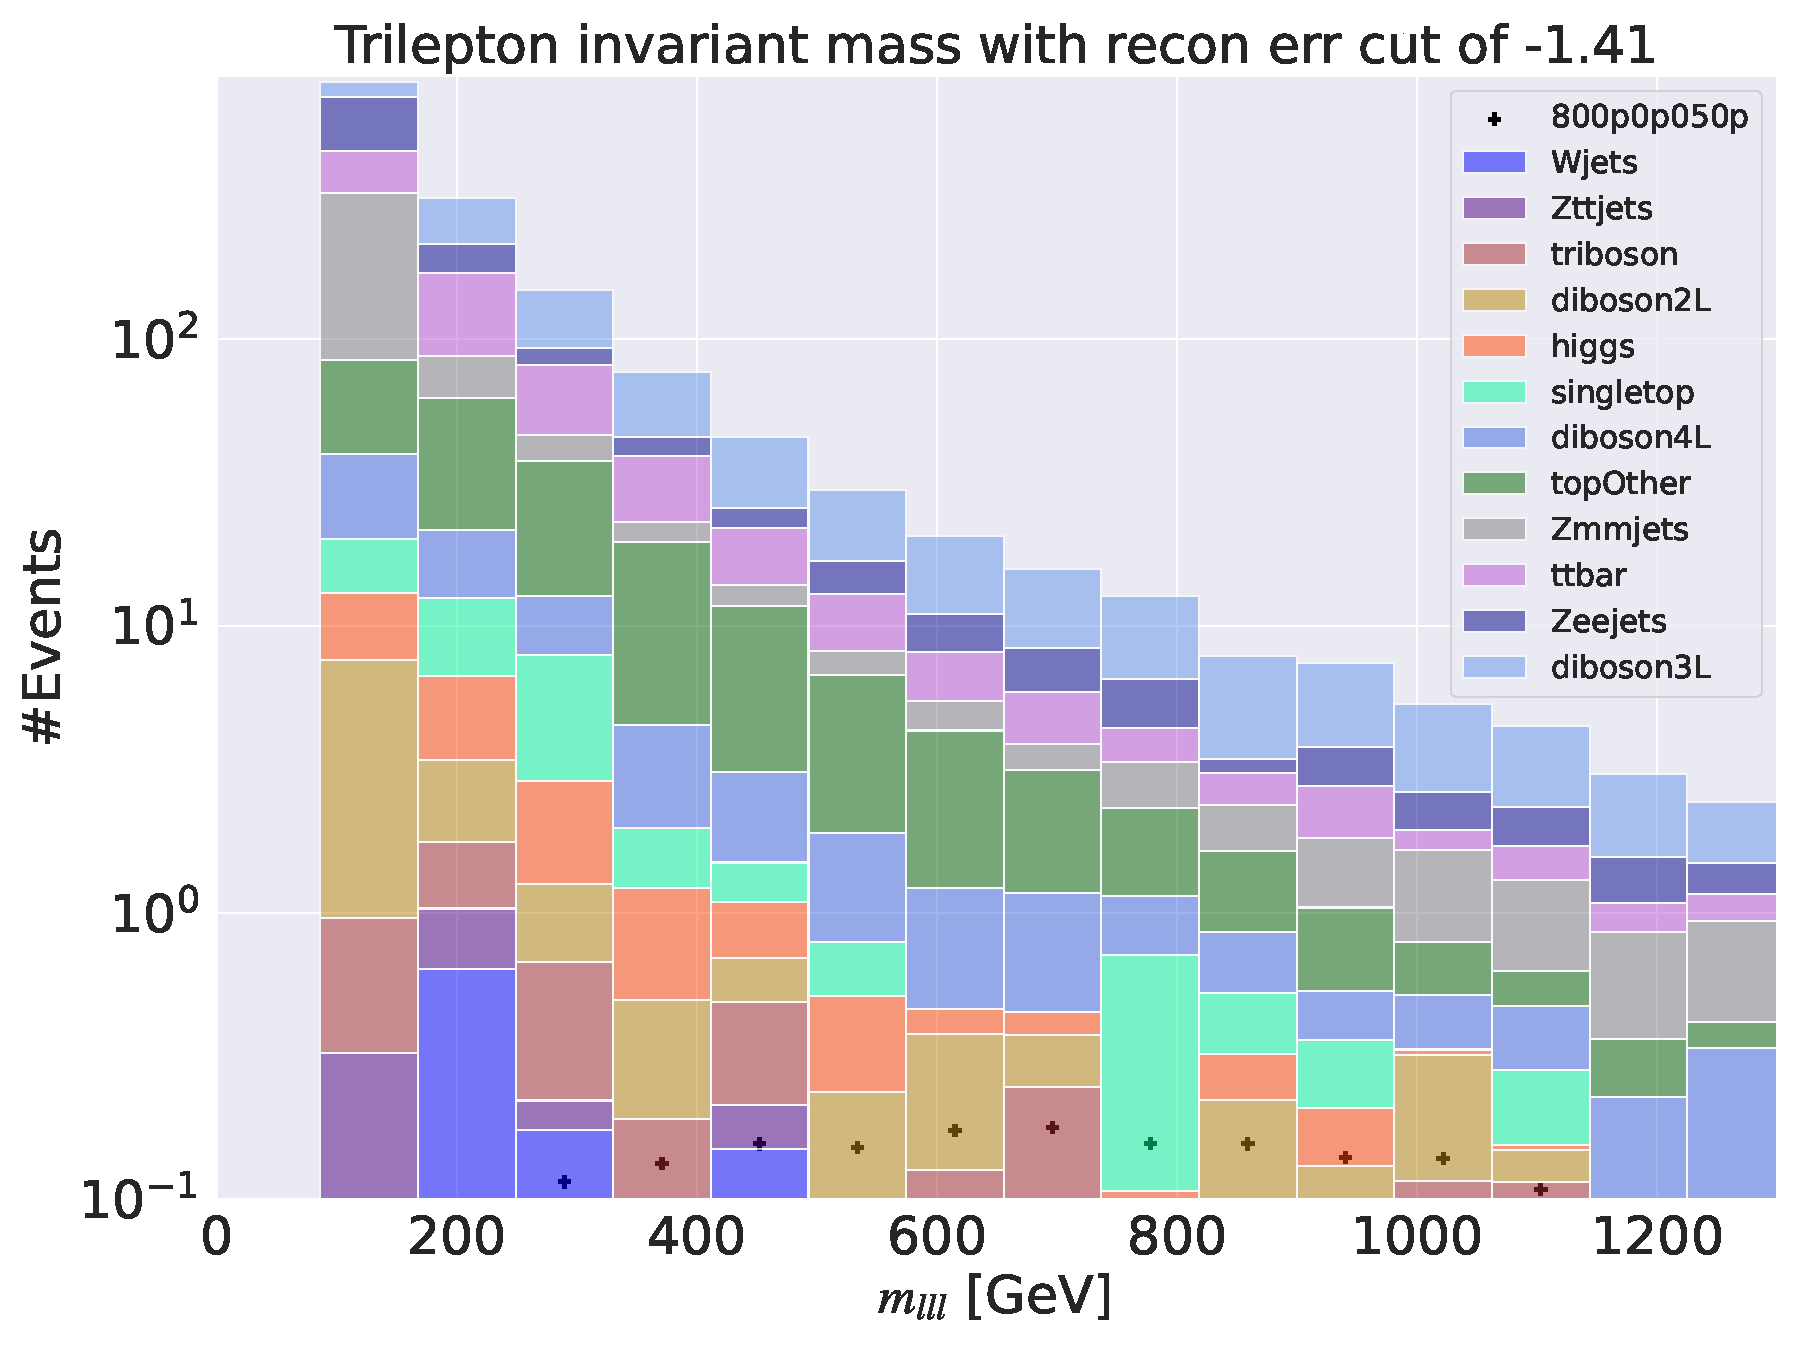
\includegraphics[width=\textwidth]{Figures/AE_testing/small/3lep/b_data_recon_big_rm3_feats_sig_800p0p050p_mlll_recon_errcut_-1.41.pdf}
        \caption{}
        \label{fig:AE_3lep_small_mlll_800}
    \end{subfigure}
    \hfill   
    \begin{subfigure}{.49\textwidth}
        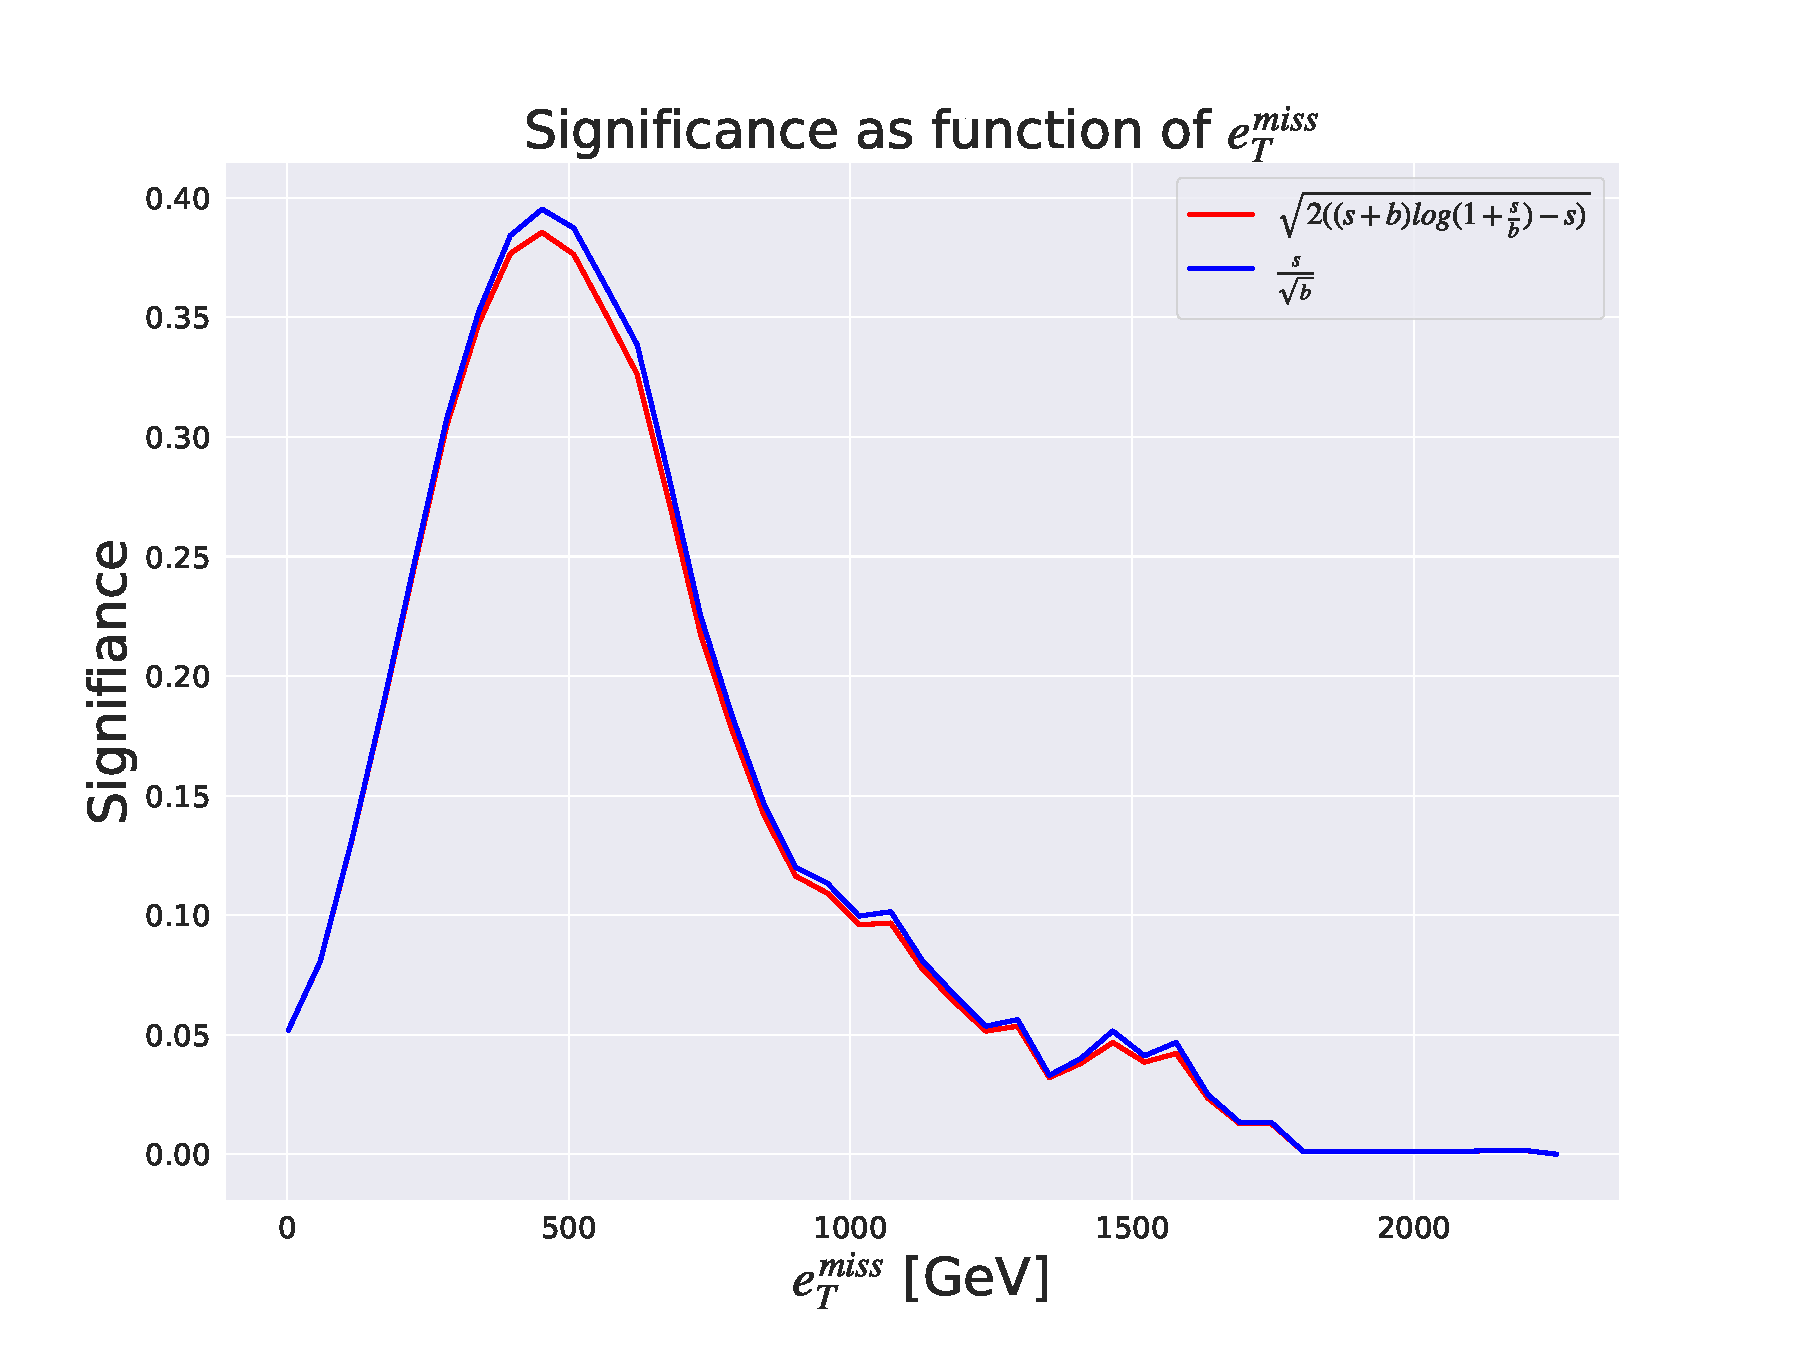
\includegraphics[width=\textwidth]{Figures/AE_testing/small/3lep/significance_etmiss_800p0p050p_-1.4089386402528896.pdf}
        \caption{}
        \label{fig:AE_3lep_small_signi_800}
    \end{subfigure}
    \hfill      
    \caption[3lep shallow network | $800p50$ | AE]{Reconstruction error, $e_T^{miss}$ signal region, $m_{lll}$ signal region and significance as function of 
    $e_T^{miss}$ for the shallow regular autoencoder using the SUSY $800p50$. 
    Figure \ref{fig:AE_3lep_small_800} shows the reconstruction error 
    distribution for the SM MC and the SUSY signal. Here the autoencoder produces a mirrored reconstruction error shape for background and 
    signal. The peaks of the two distributions are separated with two orders of magnitude in reconstruction error. Figure \ref{fig:AE_3lep_small_etmiss_800} 
    shows the $e_T^{miss}$ distribution for the SM MC and the SUSY signal in the signal region. 
    The signal region is made using a cut around $10^{-1.41}$. Most of the background is removed, and the peaks of the SM MC and signal 
    distributions are separated. Figure \ref{fig:AE_3lep_small_mlll_800} shows the $m_{lll}$ distribution for the SM MC and the SUSY signal. 
    The shape of both distributions are somewhat separated. Figure \ref{fig:AE_3lep_small_signi_800} shows the significance as function of
    $e_T^{miss}$. The peak is put around a cut of about 450 GeV in the $e_T^{miss}$, with a significance of around $0.39$.}
    \label{fig:AE_3lep_small_rec_sig_signi_800}
\end{figure}

Figures \ref{fig:AE_3lep_big_rec_sig_signi_450}, \ref{fig:AE_3lep_small_rec_sig_signi_450}, 
\ref{fig:AE_3lep_big_rec_sig_signi_800} and \ref{fig:AE_3lep_small_rec_sig_signi_800} contain four 
subplots with the total reconstruction error distributions (a), the $e_T^{miss}$ signal region (b), 
the $m_{lll}$ signal region (c) and the significance as function of $e_T^{miss}$ curve (d) respectively 
for the shallow and deep regular autoencoder. From figures \ref{fig:AE_3lep_big_450}, 
\ref{fig:AE_3lep_small_450}, \ref{fig:AE_3lep_big_800}, \ref{fig:AE_3lep_small_800} it is shown that the 
SUSY $800p50$ signals has the best separation of peaks, which is expected considering its 
rather extreme tail in the $e_T^{miss}$ distribution of the signal. It is interesting to 
observe the slope in the SM MC reconstruction error distribution. The steepness of the 
slope seems to be somewhat similar for both the shallow and deep regular autoencoders, indicating 
at least that the difference in these two models does not differ much when it comes to performance. 
The bulk of the events are below $10^{-2}$ reconstruction error, indicating that the autoencoder 
has learned a lot of the internal RMM structures for the 3 lepton + $e_T^{miss}$ final state MC. \par
In figures \ref{fig:AE_3lep_big_etmiss_450}, \ref{fig:AE_3lep_small_etmiss_450}, 
\ref{fig:AE_3lep_big_etmiss_800} and  \ref{fig:AE_3lep_small_etmiss_800} we have a signal region 
created for each of the SUSY models from both the shallow and deep regular autoencoder. The cuts 
were created using the median and then iteratively increasing the error requirement, as 
explained in section \ref{sec:strategy}. Only one of the three cuts done are shown here, the 
rest can be found in the appendix. The histograms in these figures \ref{fig:AE_3lep_big_etmiss_450}, 
\ref{fig:AE_3lep_small_etmiss_450}, \ref{fig:AE_3lep_big_etmiss_800} and  
\ref{fig:AE_3lep_small_etmiss_800} display the $e_T^{miss}$ distribution in the signal region 
for the SM MC and the SUSY signals. They represent the signal region with the most relaxed cut, 
in other words, the least strict and thus the signal region with the highest amount of events, 
both SM MC and signal. This is to illustrate the difficulty of this method since we do not have 
any idea how anomalous (i.e. how large reconstruction error) we expect a BSM signal to have. 
Thus, a too strict a cut will most likely eliminate all possible 
signal events in the signal region, whereas a too loose a cut would result in the SM MC background dominating completely. \par
In figures \ref{fig:AE_3lep_big_mlll_450}, \ref{fig:AE_3lep_small_mlll_450}, \ref{fig:AE_3lep_big_mlll_800} and  
\ref{fig:AE_3lep_small_mlll_800} we have the  $m_{lll}$ distributions in the signal 
regions from both the shallow and deep regular 
autoencoder for both SUSY signals. As with the $e_T^{miss}$ distributions, the $m_{lll}$ distributions 
with the least strict cut in the signal region are shown here, with the rest shown in the appendix. 
It is shown that the difference between the shallow and deep neural network architecture has little to no effect 
here or in the $e_T^{miss}$ distributions in terms of separation. \par 
In figures \ref{fig:AE_3lep_big_signi_450}, \ref{fig:AE_3lep_small_signi_450}, \ref{fig:AE_3lep_big_signi_800} and  
\ref{fig:AE_3lep_small_signi_800} we have the significance as a function of the $e_T^{miss}$. It displays that 
a further cut on the $e_T^{miss}$ will get an even better significance. The best case is provided from the SUSY $450p300$
signal with the deep autoencoder, applying a cut on the $e_T^{miss}$ around 380 GeV, leading to a significance of $0.78$. 


\subsubsection*{Variational autoencoder output}


\begin{figure}[h!]
    \centering
    \begin{subfigure}{.49\textwidth}
        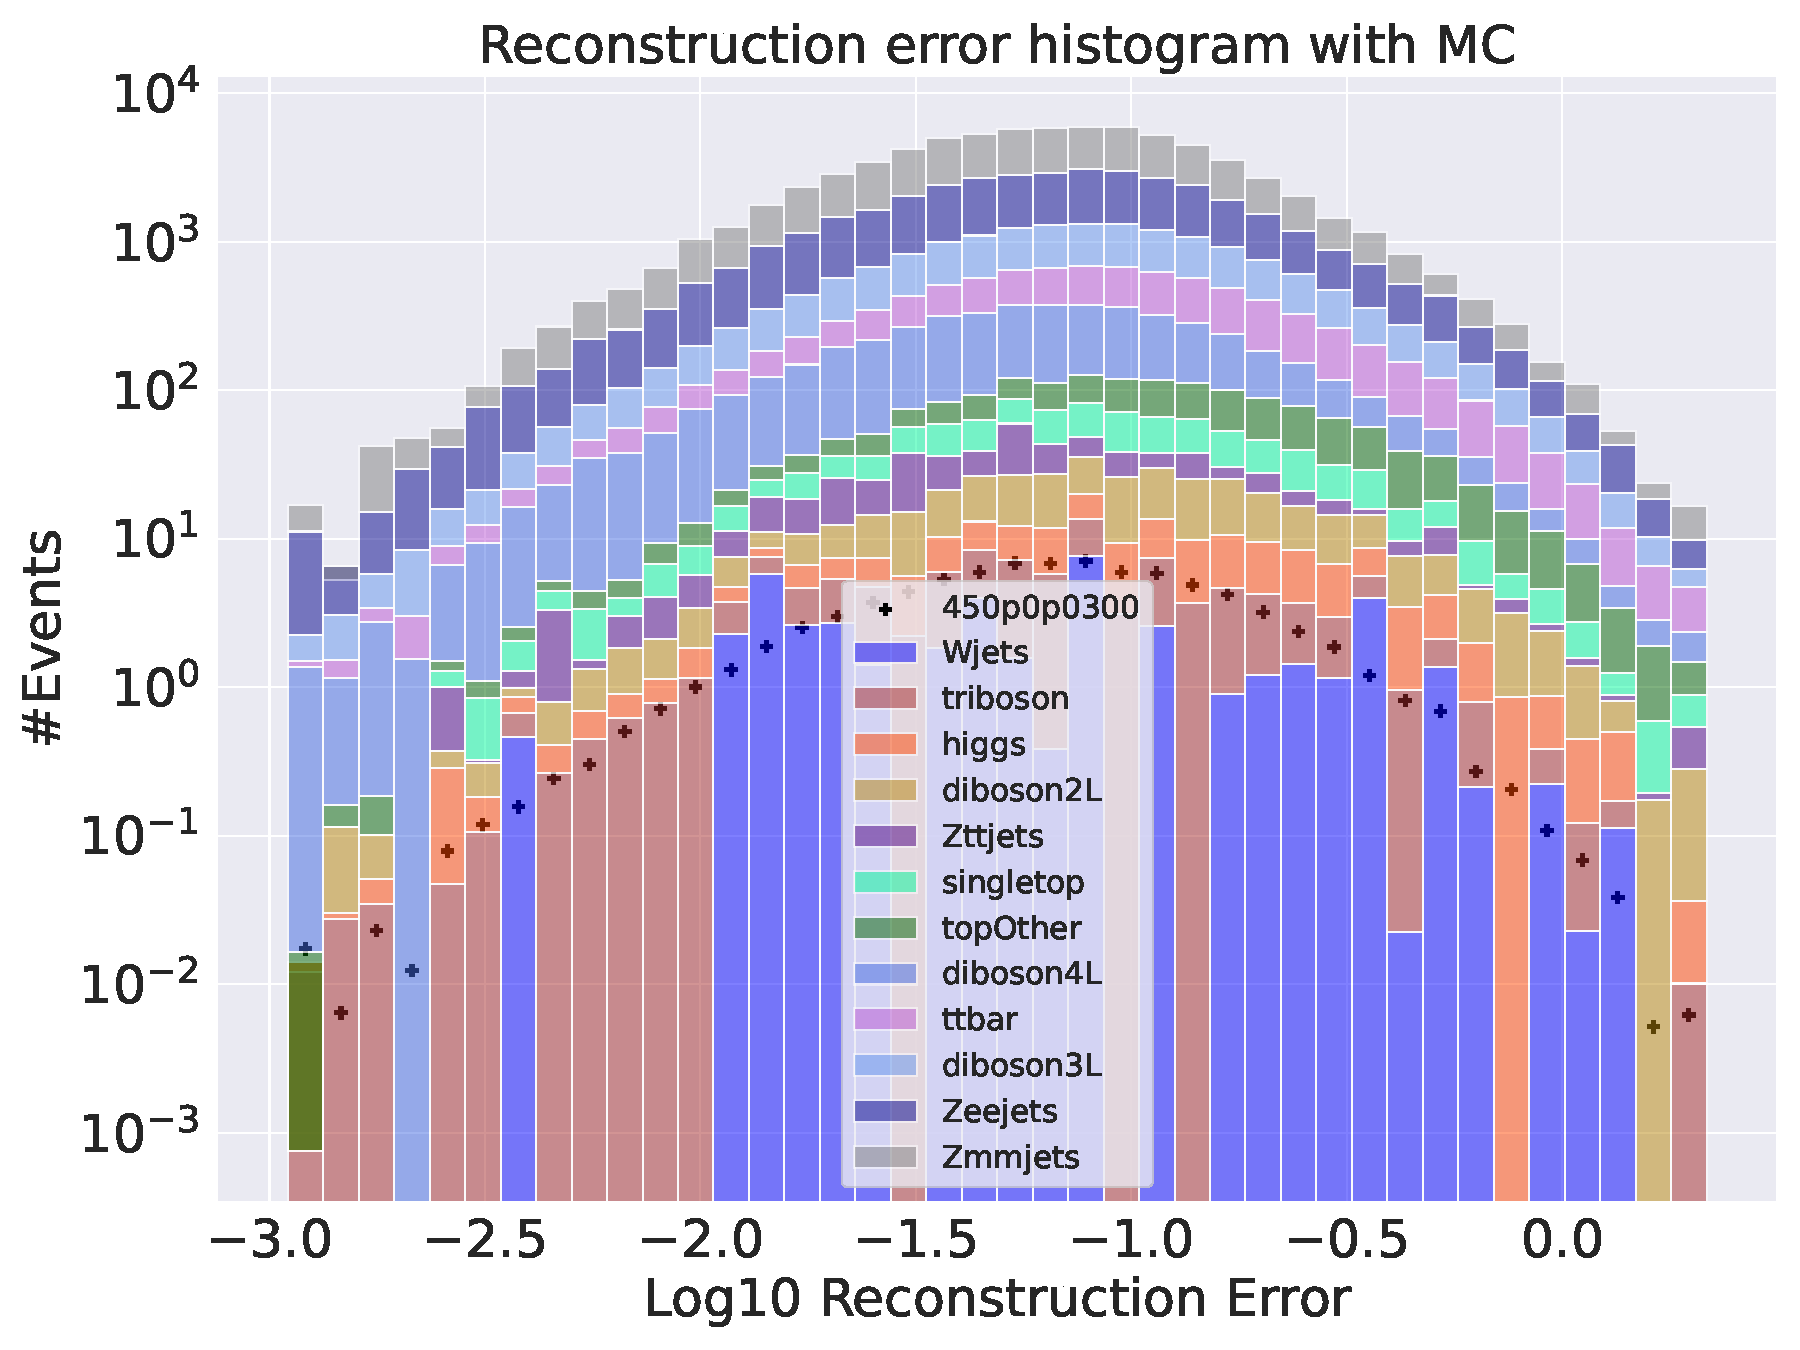
\includegraphics[width=\textwidth]{Figures/VAE_testing/big/3lep/b_data_recon_big_rm3_feats_sig_450p0p0300.pdf}
        \caption{ }
        \label{fig:VAE_3lep_big_450}
    \end{subfigure}
    \hfill
    \begin{subfigure}{.49\textwidth}
        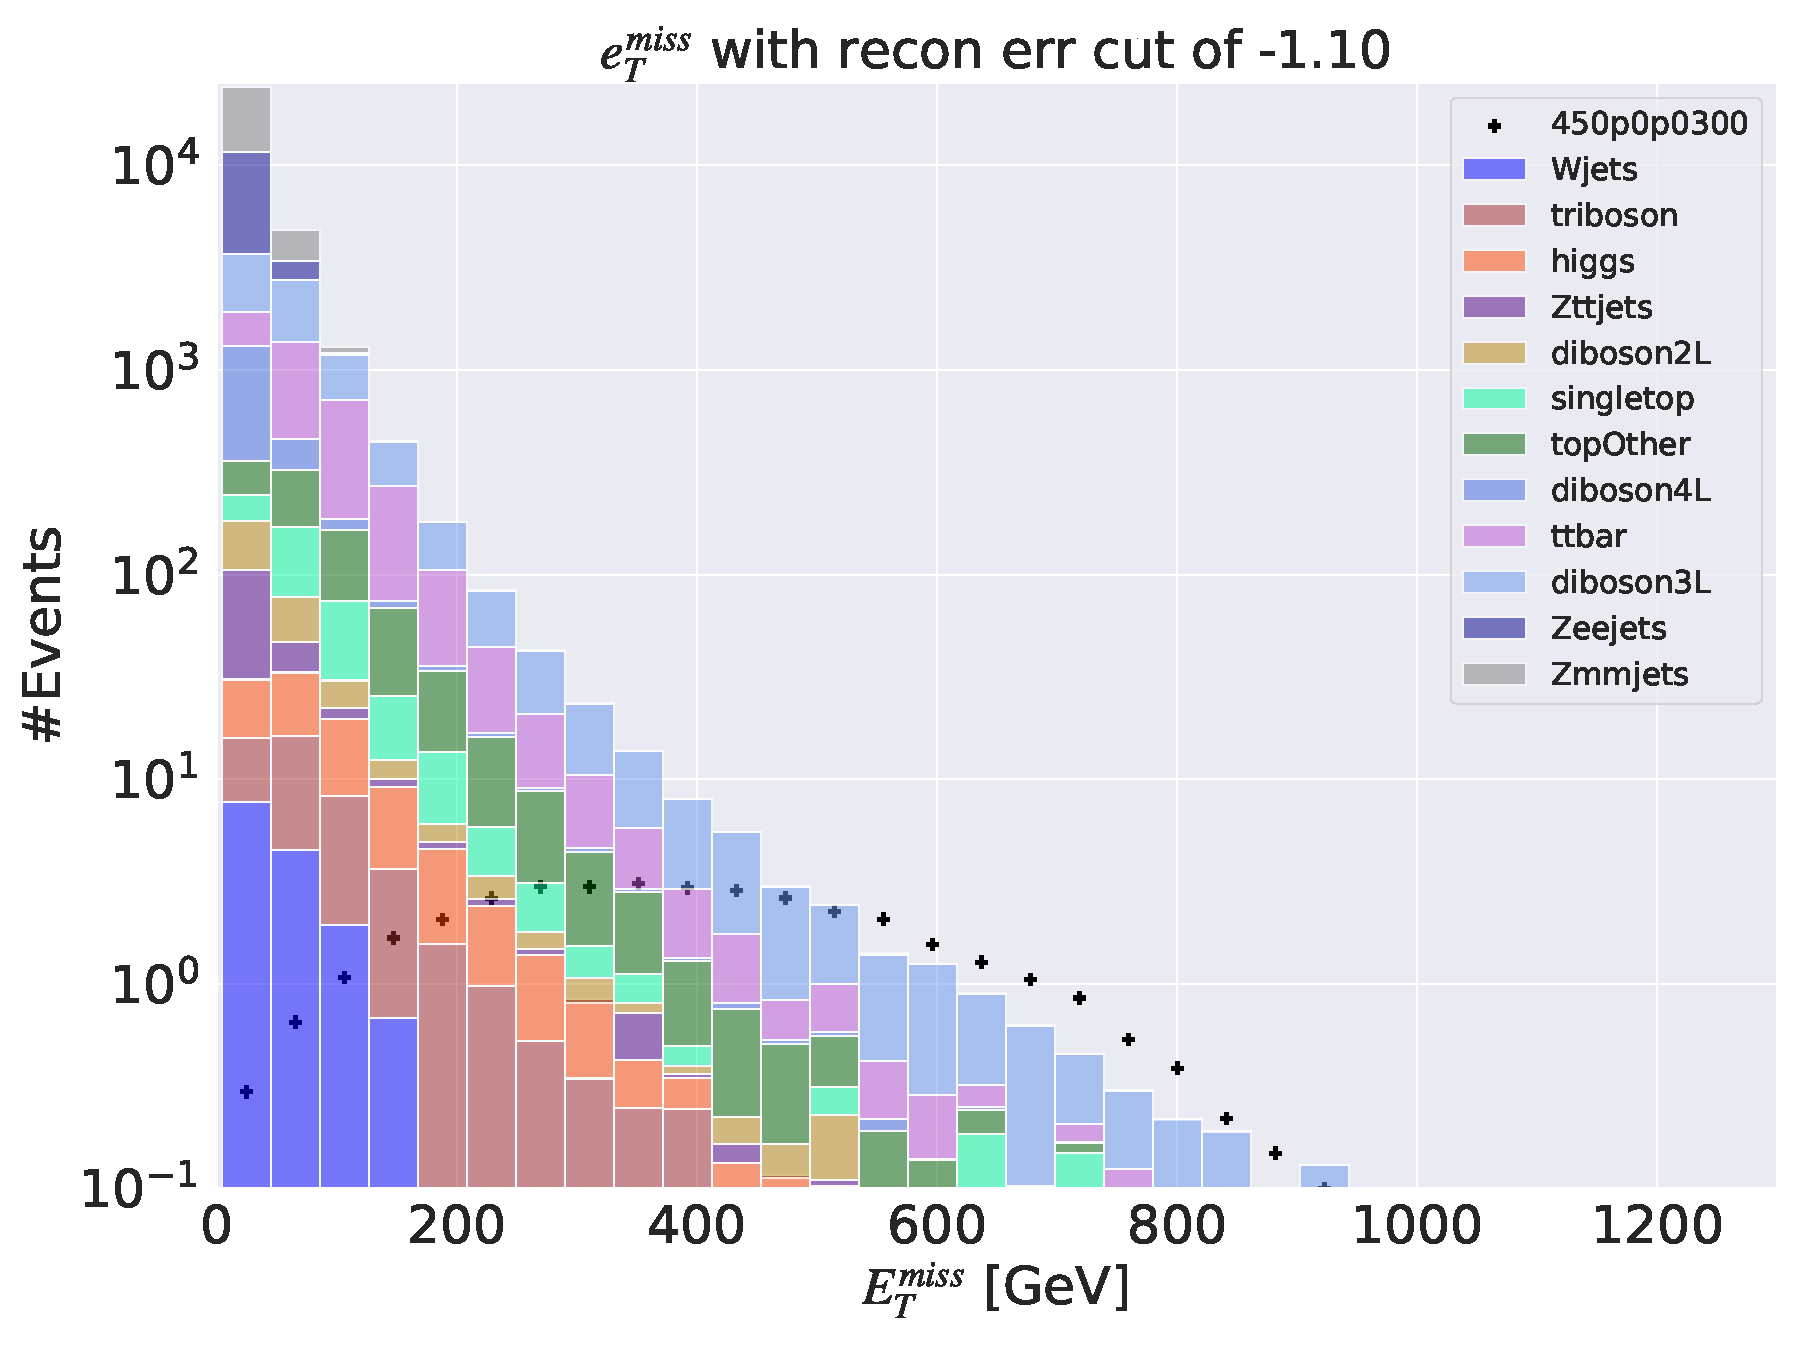
\includegraphics[width=\textwidth]{Figures/VAE_testing/big/3lep/b_data_recon_big_rm3_feats_sig_450p0p0300_etmiss_recon_errcut_-1.10.pdf}
        \caption{}
        \label{fig:VAE_3lep_big_etmiss_450}
    \end{subfigure}
    \hfill
    \begin{subfigure}{.49\textwidth}
        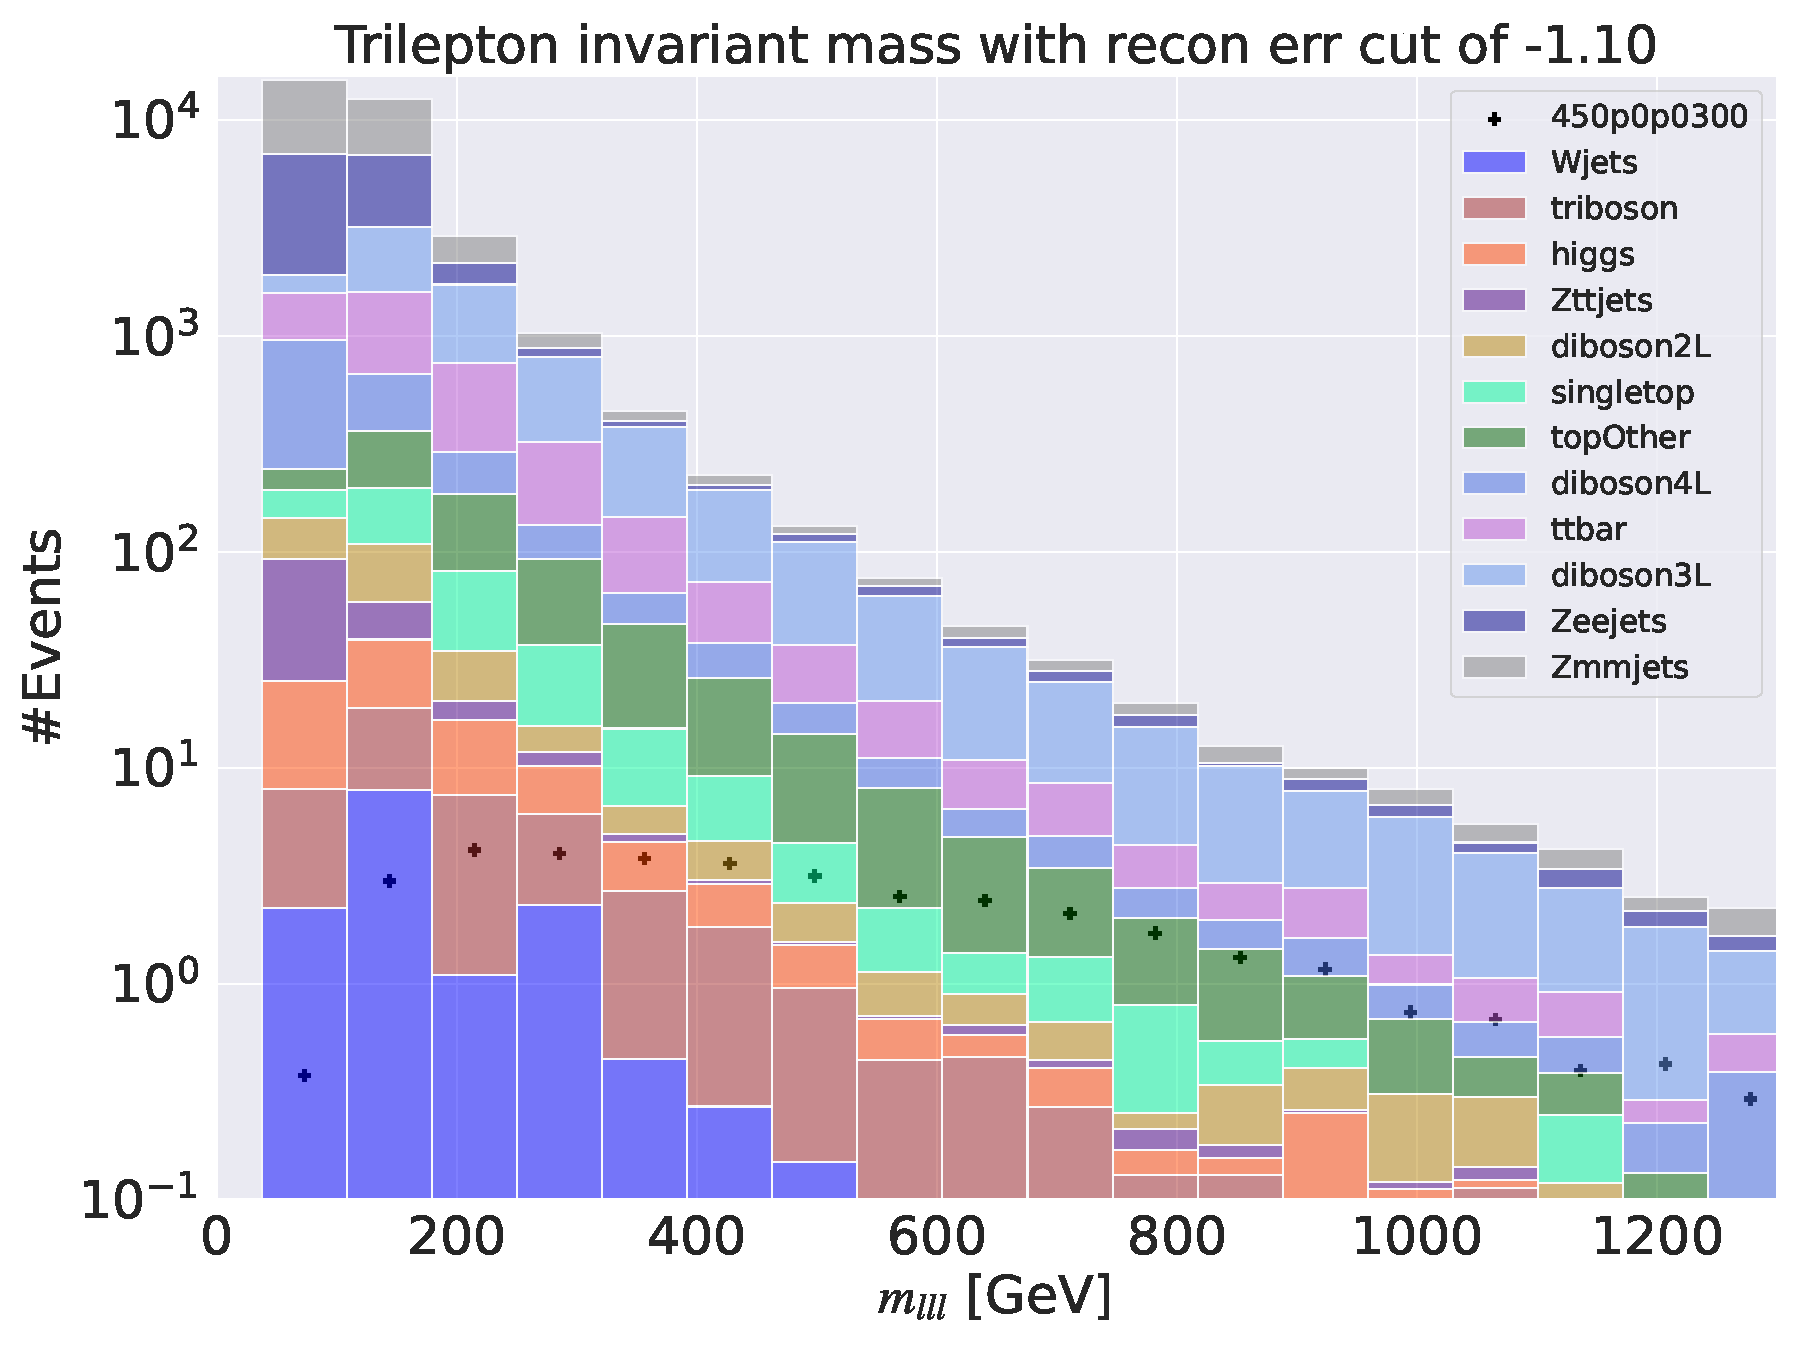
\includegraphics[width=\textwidth]{Figures/VAE_testing/big/3lep/b_data_recon_big_rm3_feats_sig_450p0p0300_mlll_recon_errcut_-1.10.pdf}
        \caption{}
        \label{fig:VAE_3lep_big_mlll_450}
    \end{subfigure}
    \hfill   
    \begin{subfigure}{.49\textwidth}
        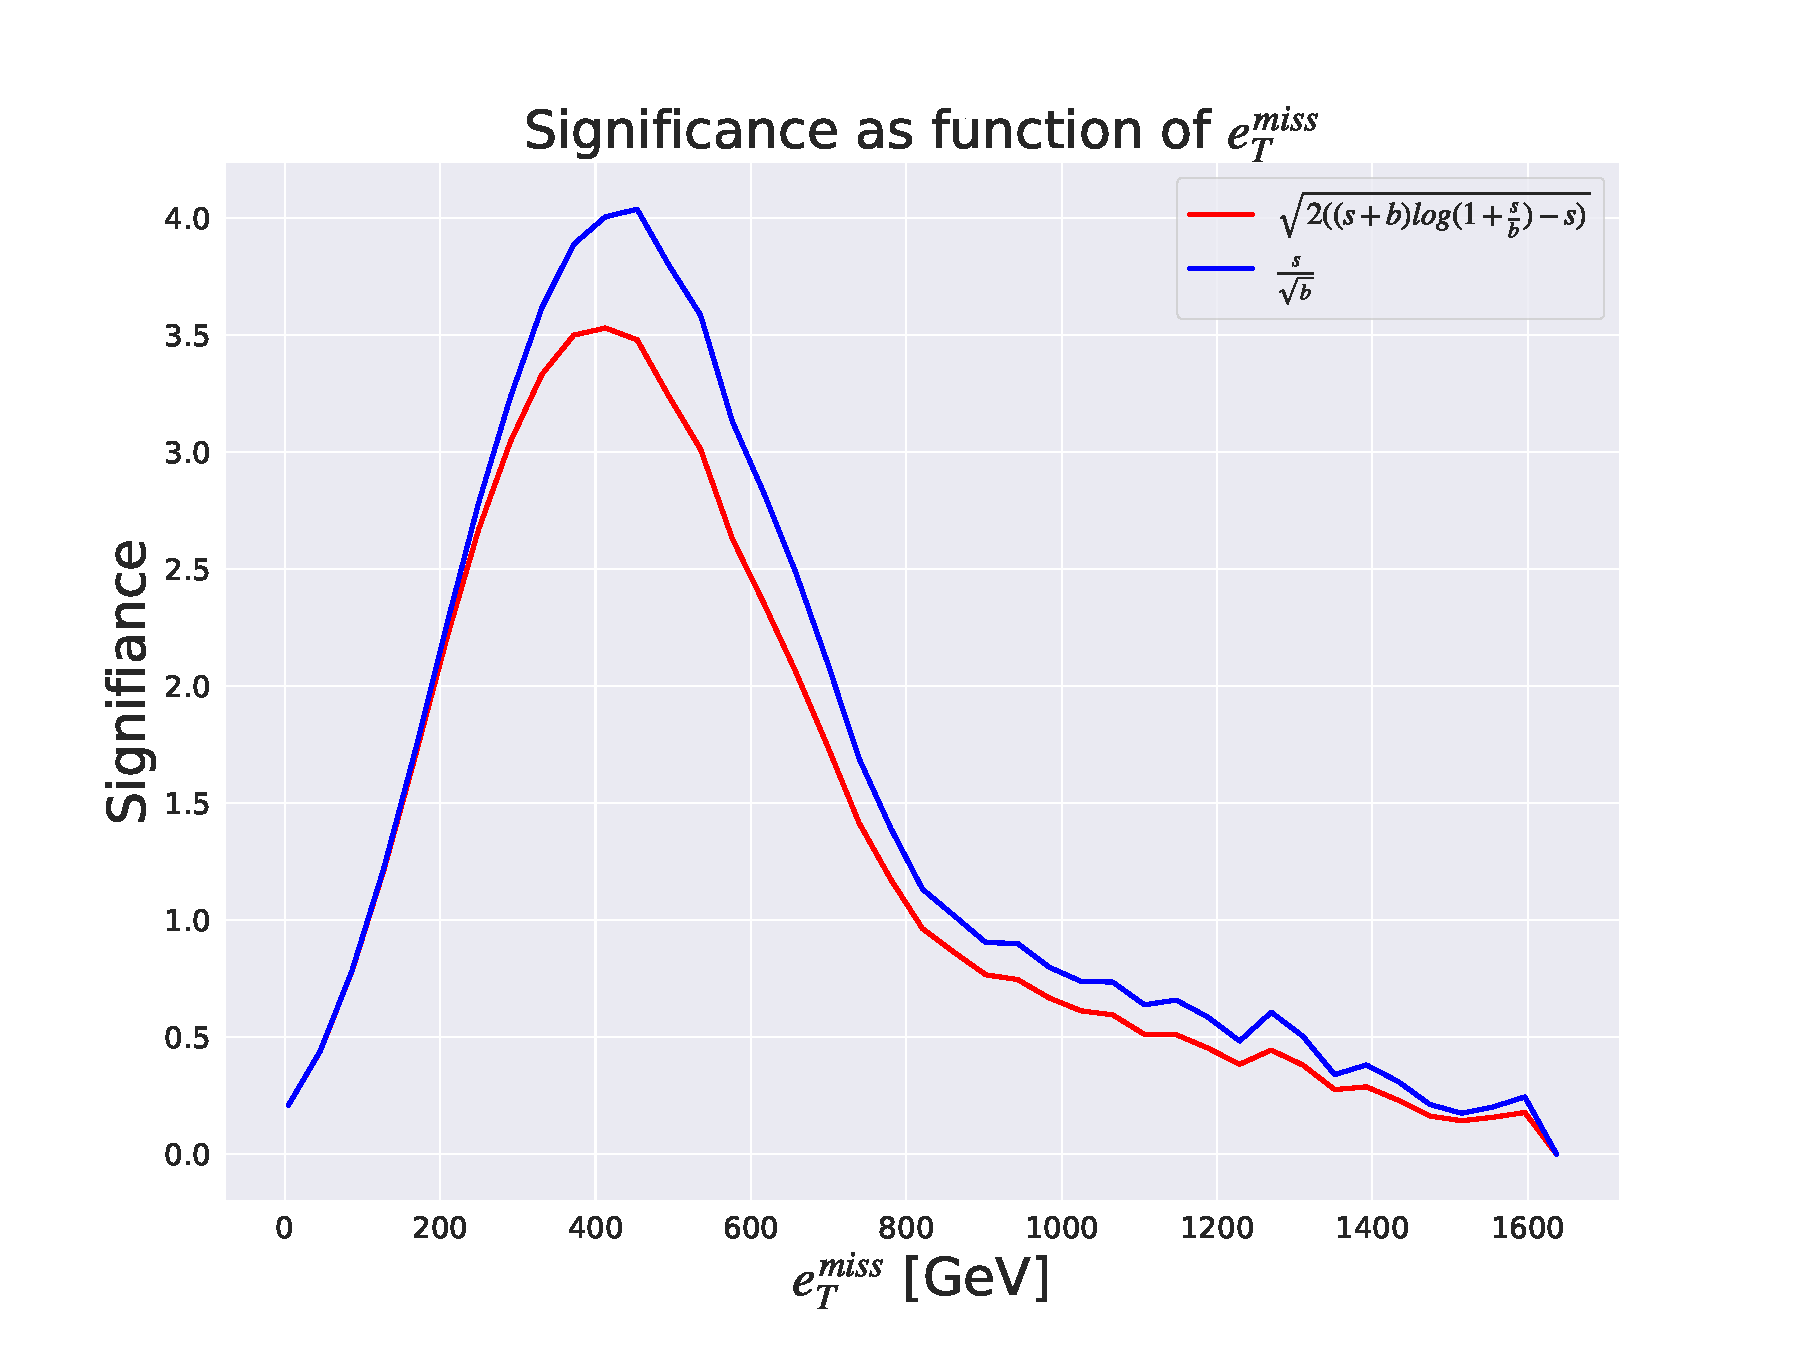
\includegraphics[width=\textwidth]{Figures/VAE_testing/big/3lep/significance_etmiss_450p0p0300_-1.0969148715571329.pdf}
        \caption{}
        \label{fig:VAE_3lep_big_signi_450}
    \end{subfigure}
    \hfill      
    \caption[3lep deep network | $450p300$ | VAE]{Reconstruction error, $e_T^{miss}$ signal region, $m_{lll}$ signal region and significance as function of 
    $e_T^{miss}$ for the deep variational autoencoder using the SUSY $450p300$.
    Figure \ref{fig:VAE_3lep_big_450} shows the reconstruction error 
    distribution for the SM MC and the SUSY signal. Here the autoencoder produces a hill-like for background and 
    signal with little destinction. The peaks of the two distributions are not separated in reconstruction error. Figure \ref{fig:VAE_3lep_big_etmiss_450} 
    shows the $e_T^{miss}$ distribution for the SM MC and the SUSY signal in the signal region. 
    The signal region is made using a cut around $10^{-1.10}$. Some background is removed, and the peaks of the SM MC and signal 
    distributions are separated. Figure \ref{fig:VAE_3lep_big_mlll_450} shows the $m_{lll}$ distribution for the SM MC and the SUSY signal. 
    The shape of both distributions are displaying almost the same shape. Figure \ref{fig:VAE_3lep_big_signi_450} shows the significance as 
    function of $e_T^{miss}$. The peak is put around a cut of about 450 GeV in the $e_T^{miss}$, with a significance of around $4.1$.}
    \label{fig:VAE_3lep_big_rec_sig_signi_450}
\end{figure}

\begin{figure}[h!]
    \centering
    \begin{subfigure}{.49\textwidth}
        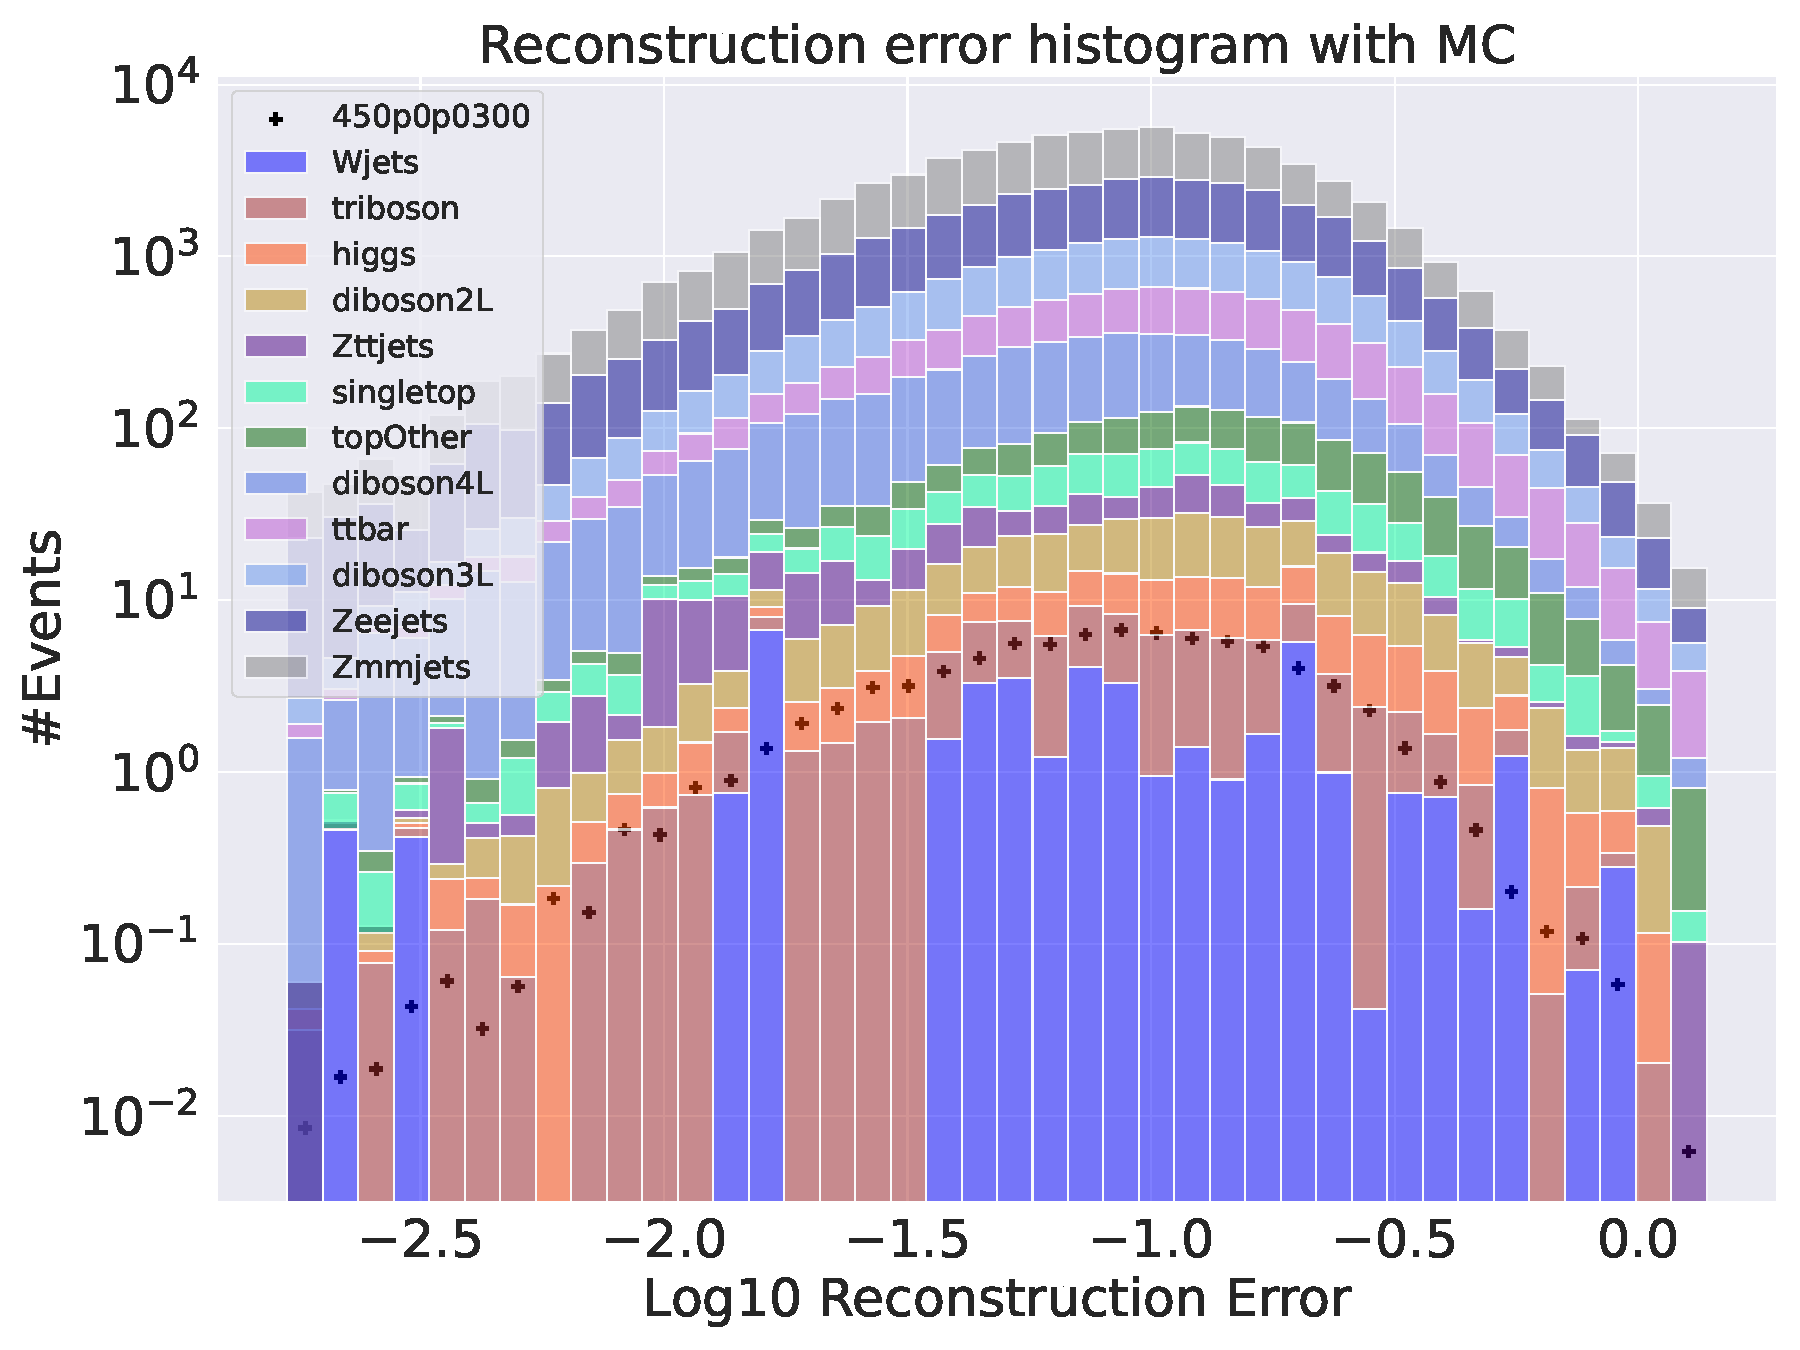
\includegraphics[width=\textwidth]{Figures/VAE_testing/small/3lep/b_data_recon_big_rm3_feats_sig_450p0p0300.pdf}
        \caption{ }
        \label{fig:VAE_3lep_small_450}
    \end{subfigure}
    \hfill
    \begin{subfigure}{.49\textwidth}
        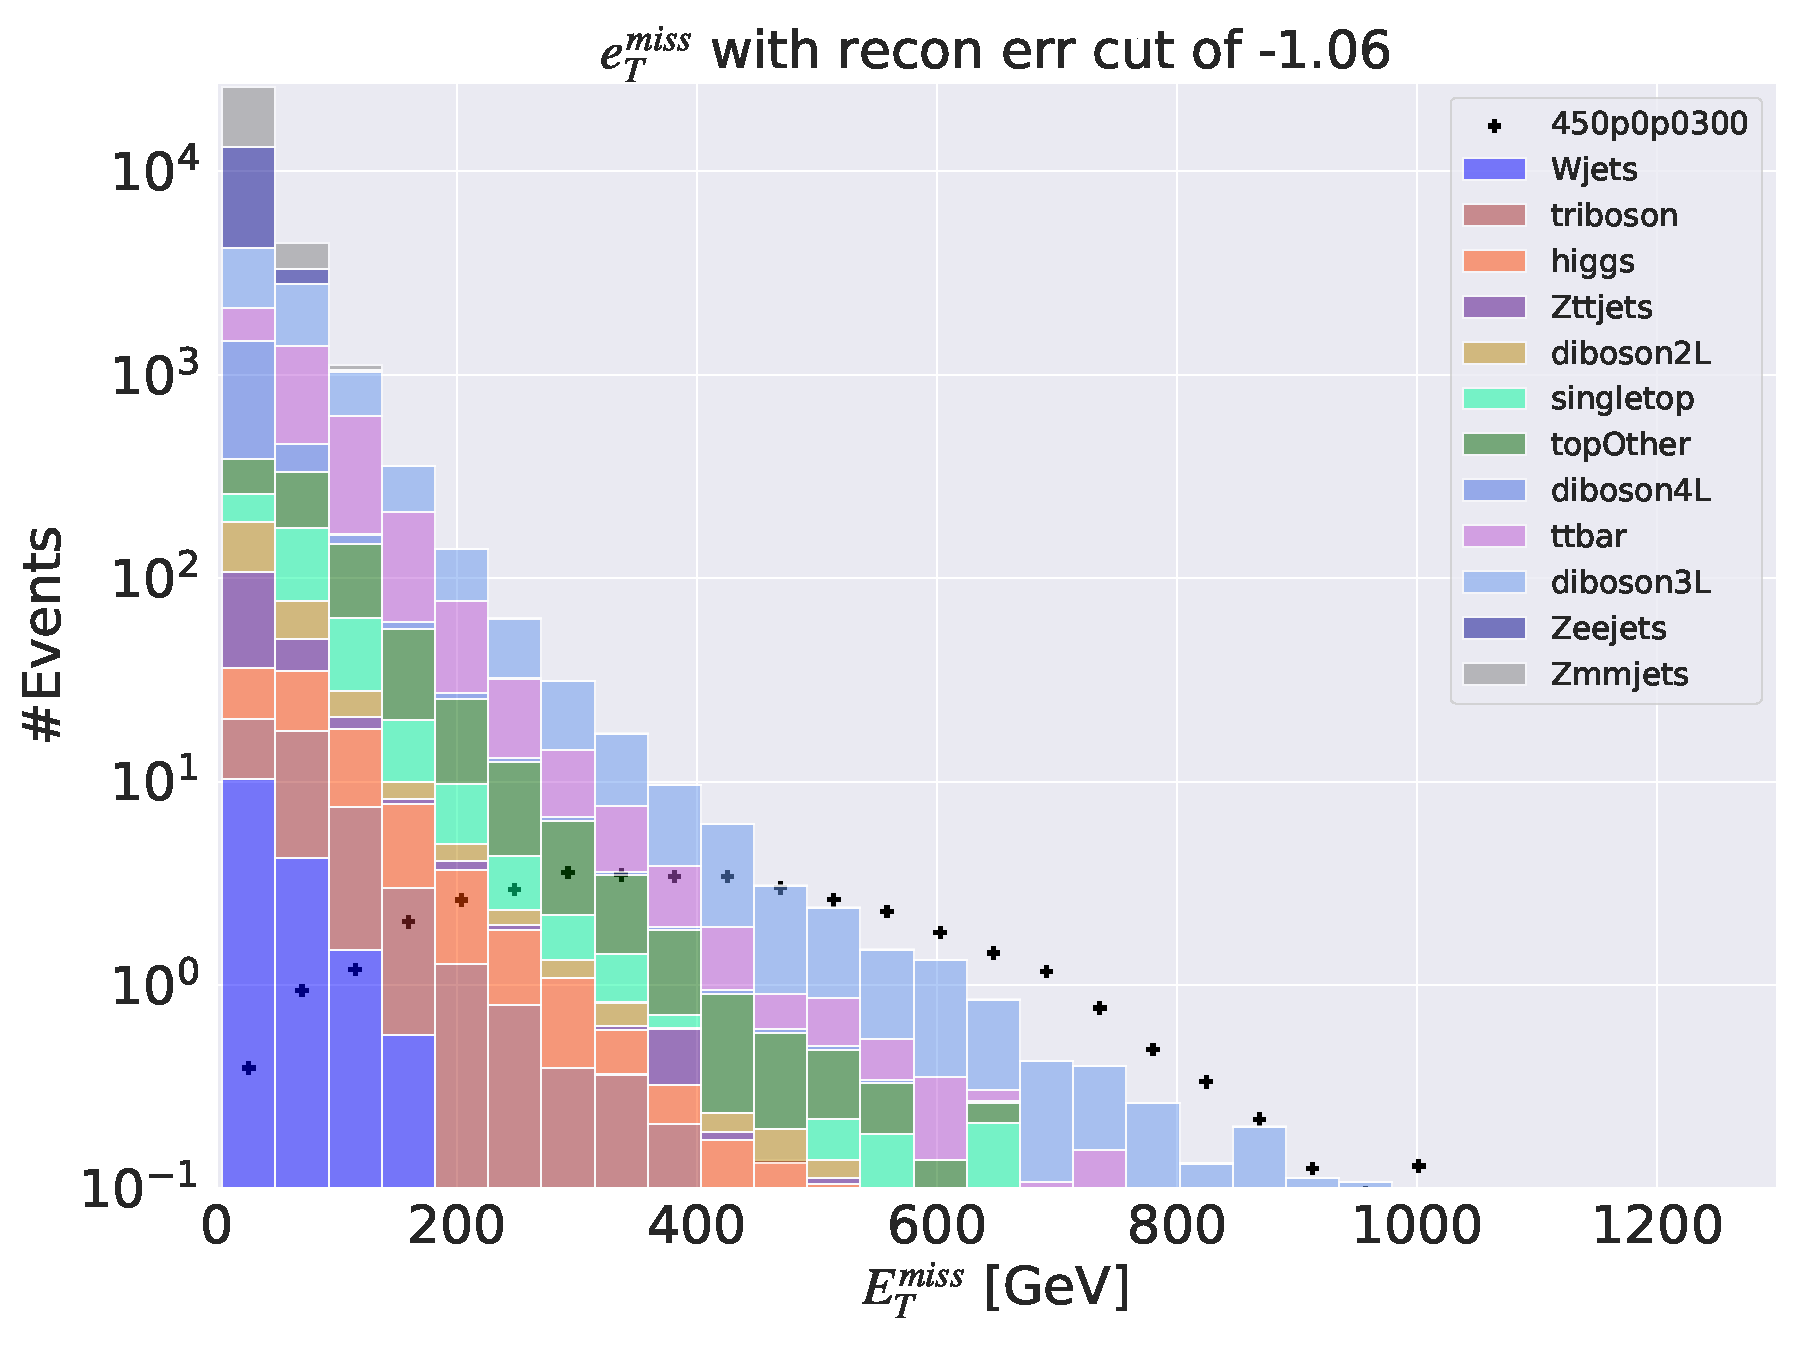
\includegraphics[width=\textwidth]{Figures/VAE_testing/small/3lep/b_data_recon_big_rm3_feats_sig_450p0p0300_etmiss_recon_errcut_-1.06.pdf}
        \caption{}
        \label{fig:VAE_3lep_small_etmiss_450}
    \end{subfigure}
    \hfill
    \begin{subfigure}{.49\textwidth}
        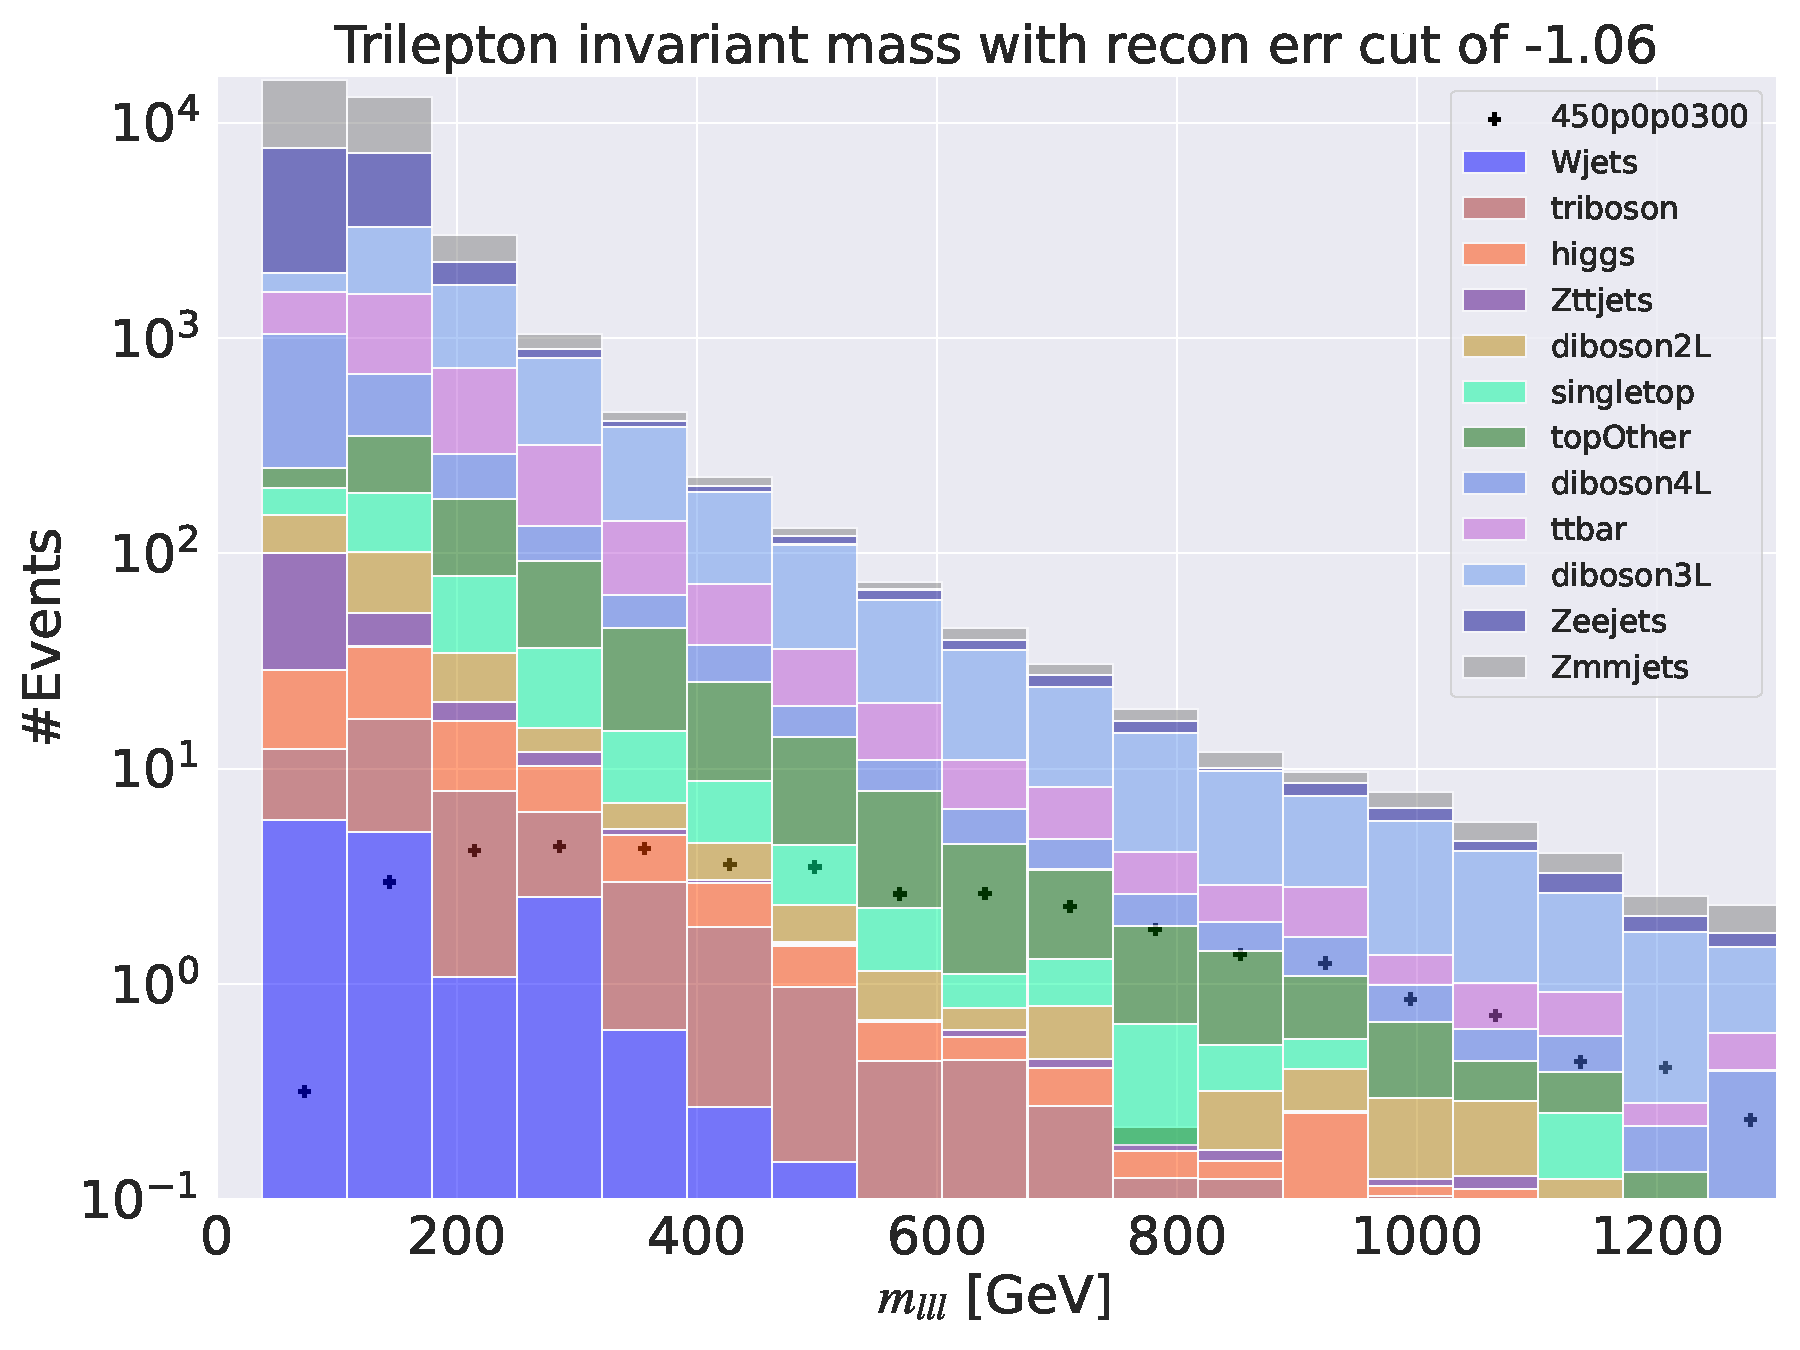
\includegraphics[width=\textwidth]{Figures/VAE_testing/small/3lep/b_data_recon_big_rm3_feats_sig_450p0p0300_mlll_recon_errcut_-1.06.pdf}
        \caption{}
        \label{fig:VAE_3lep_small_mlll_450}
    \end{subfigure}
    \hfill   
    \begin{subfigure}{.49\textwidth}
        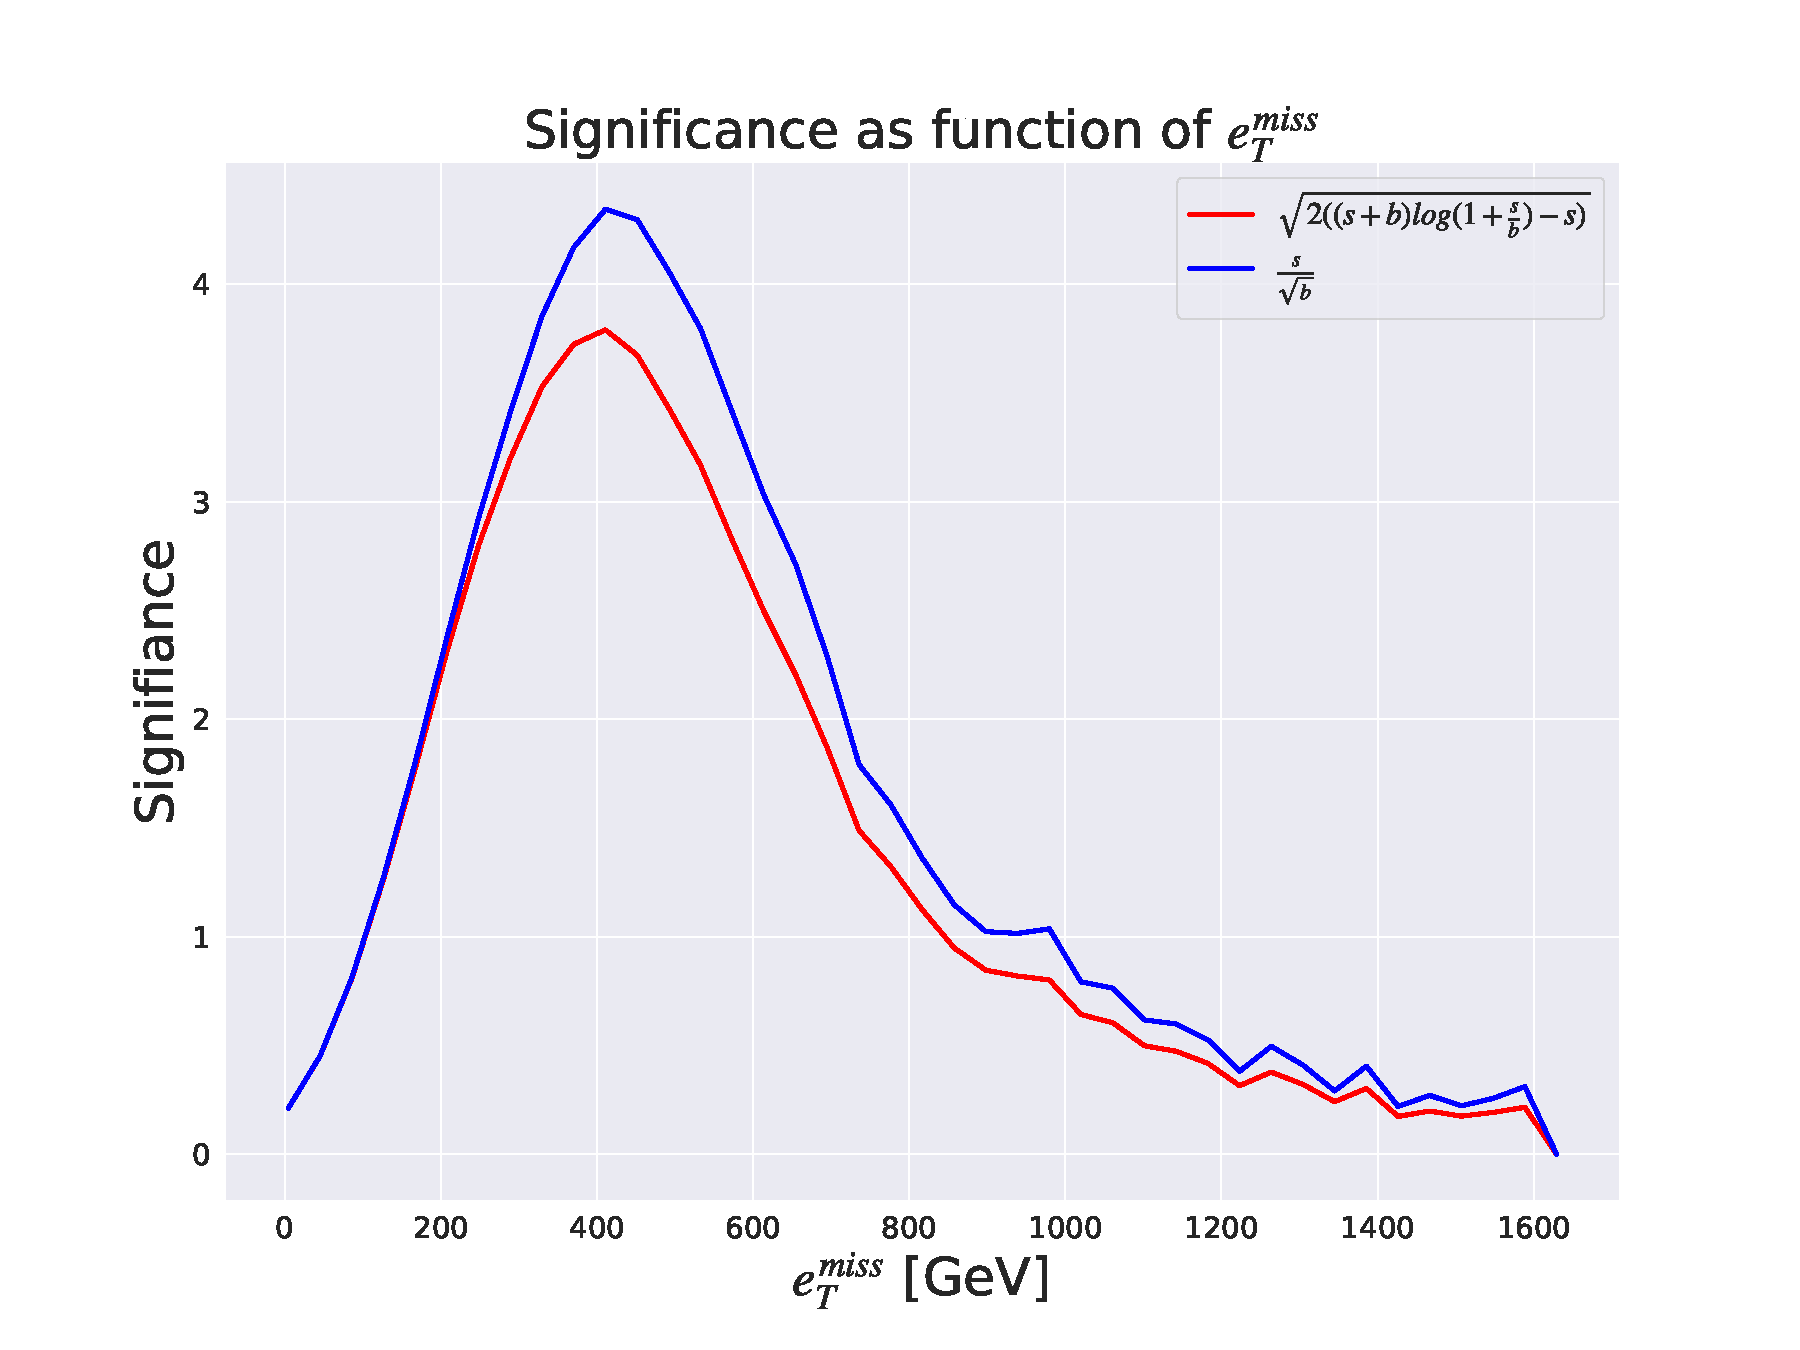
\includegraphics[width=\textwidth]{Figures/VAE_testing/small/3lep/significance_etmiss_450p0p0300_-1.0610372272331543.pdf}
        \caption{}
        \label{fig:VAE_3lep_small_signi_450}
    \end{subfigure}
    \hfill      
    \caption[3lep shallow network | $450p300$ | VAE]{Reconstruction error, $e_T^{miss}$ signal region, $m_{lll}$ signal region and significance as function of 
    $e_T^{miss}$ for the shallow variational autoencoder using the SUSY $450p300$. 
    Figure \ref{fig:VAE_3lep_small_450} shows the reconstruction error 
    distribution for the SM MC and the SUSY signal. Here the autoencoder produces a hill-like for background and 
    signal with little destinction. The peaks of the two distributions are not separated in reconstruction error. Figure \ref{fig:VAE_3lep_small_etmiss_450} 
    shows the $e_T^{miss}$ distribution for the SM MC and the SUSY signal in the signal region. 
    The signal region is made using a cut around $10^{-1.06}$. Some background is removed, and the peaks of the SM MC and signal 
    distributions are separated. Figure \ref{fig:VAE_3lep_small_mlll_450} shows the $m_{lll}$ distribution for the SM MC and the SUSY signal. 
    The shape of both distributions are displaying almost the same shape. Figure \ref{fig:VAE_3lep_small_signi_450} shows the significance as 
    function of $e_T^{miss}$. The peak is put around a cut of about 400 GeV in the $e_T^{miss}$, with a significance of around $4.5$.}
    \label{fig:VAE_3lep_small_rec_sig_signi_450}
\end{figure}








\begin{figure}[h!]
    \centering
    \begin{subfigure}{.49\textwidth}
        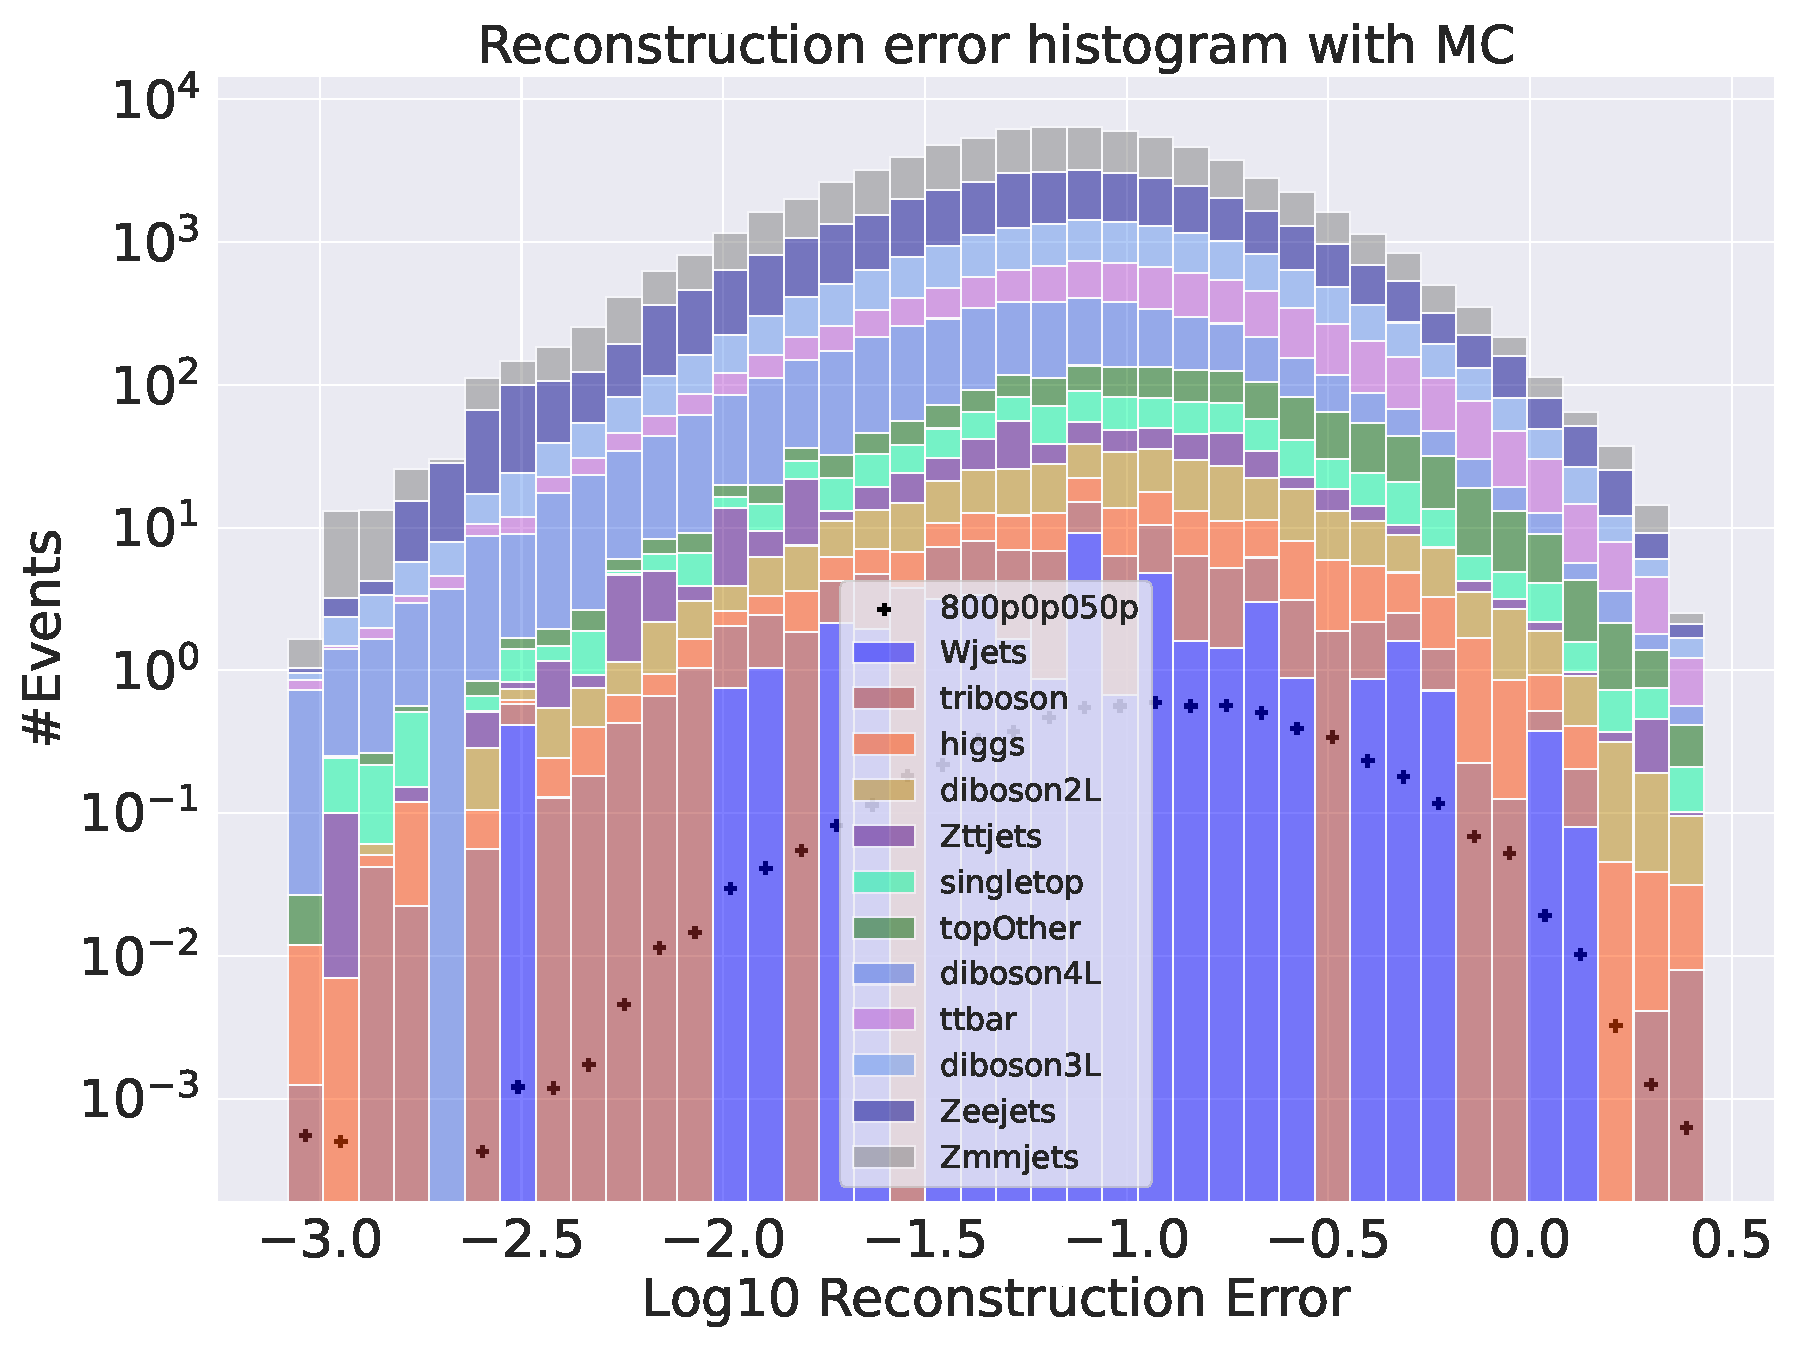
\includegraphics[width=\textwidth]{Figures/VAE_testing/big/3lep/b_data_recon_big_rm3_feats_sig_800p0p050p.pdf}
        \caption{ }
        \label{fig:VAE_3lep_big_800}
    \end{subfigure}
    \hfill
    \begin{subfigure}{.49\textwidth}
        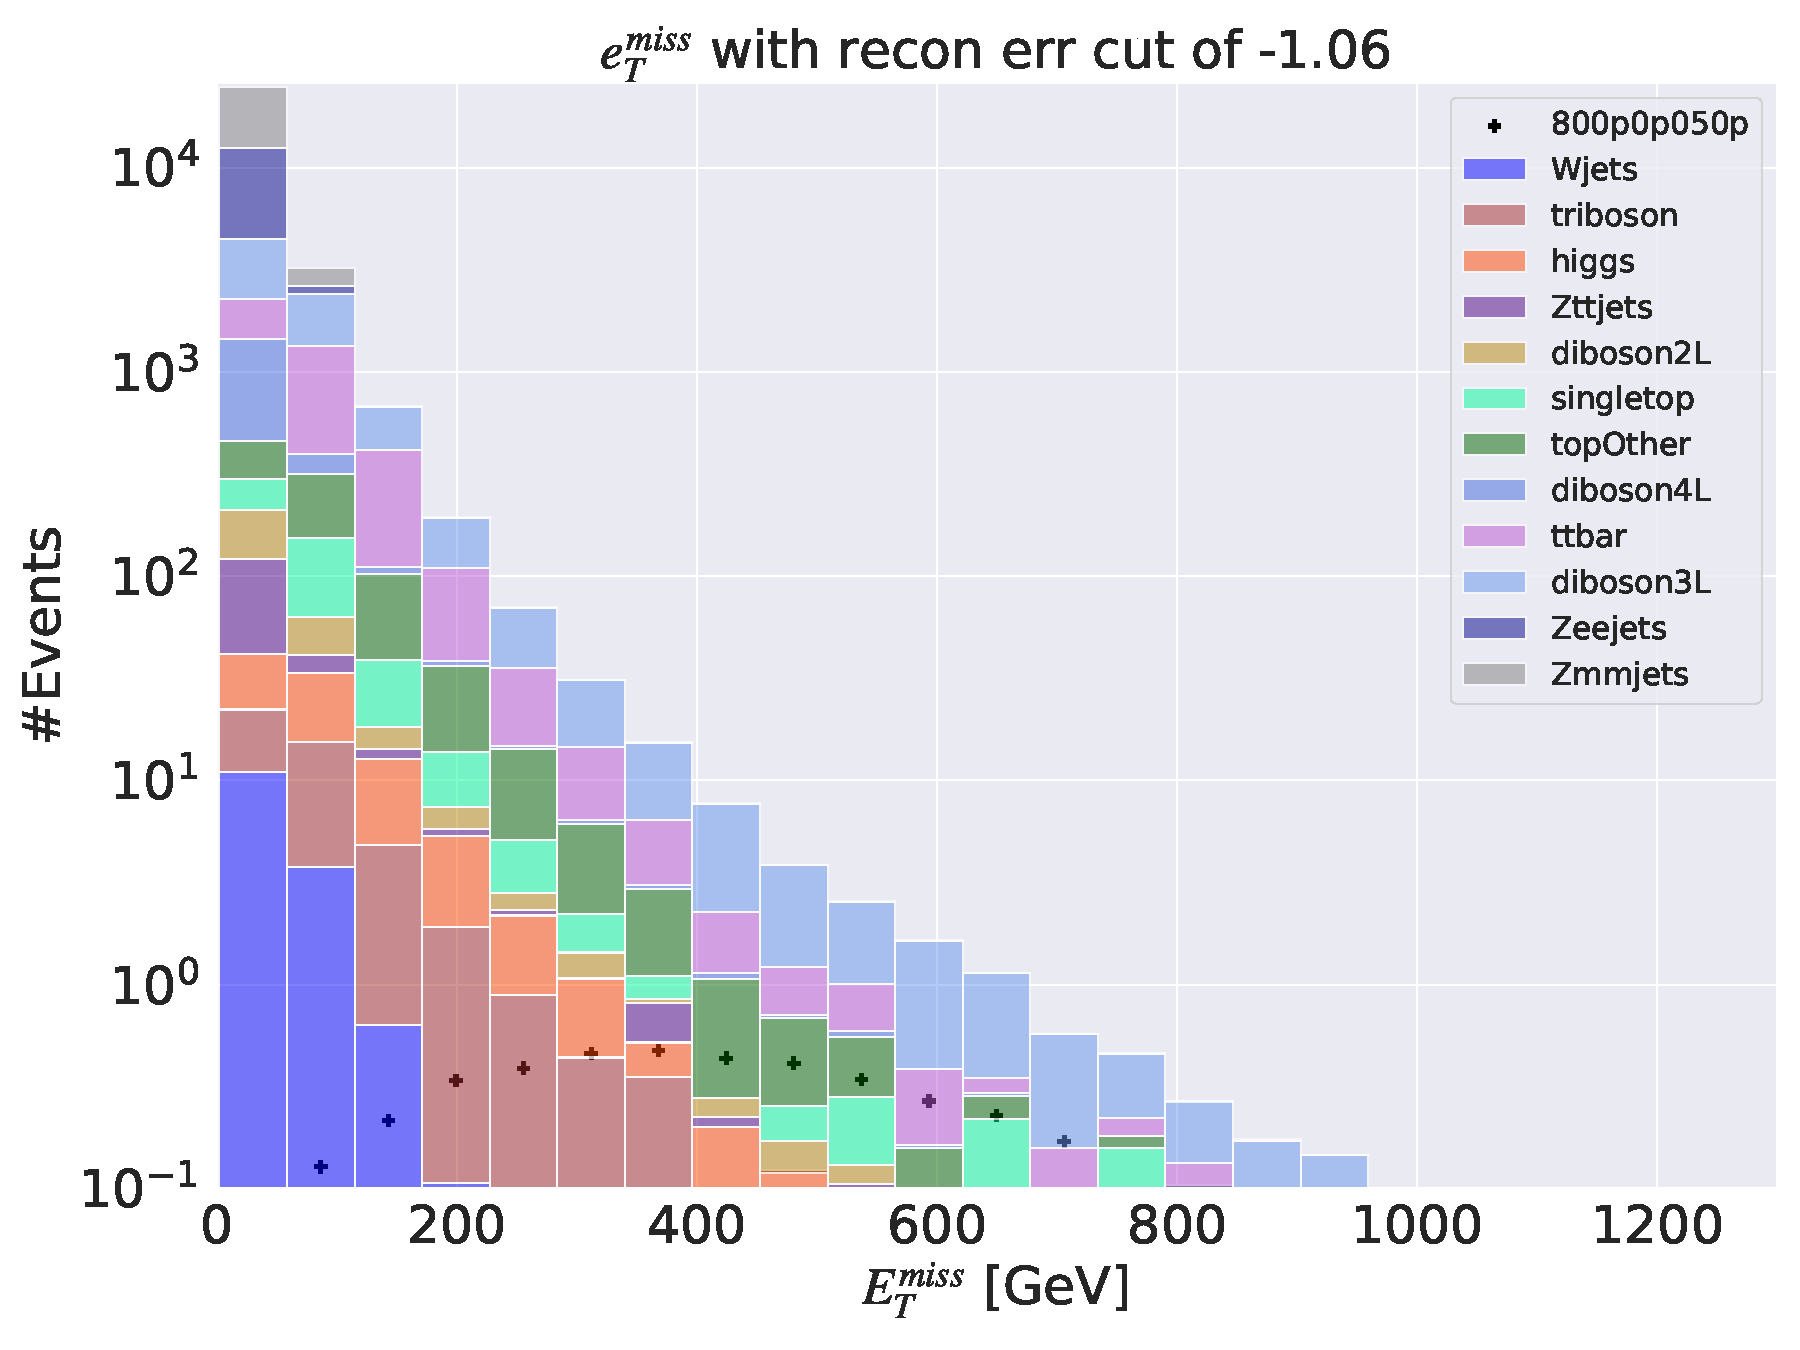
\includegraphics[width=\textwidth]{Figures/VAE_testing/big/3lep/b_data_recon_big_rm3_feats_sig_800p0p050p_etmiss_recon_errcut_-1.06.pdf}
        \caption{}
        \label{fig:VAE_3lep_big_etmiss_800}
    \end{subfigure}
    \hfill
    \begin{subfigure}{.49\textwidth}
        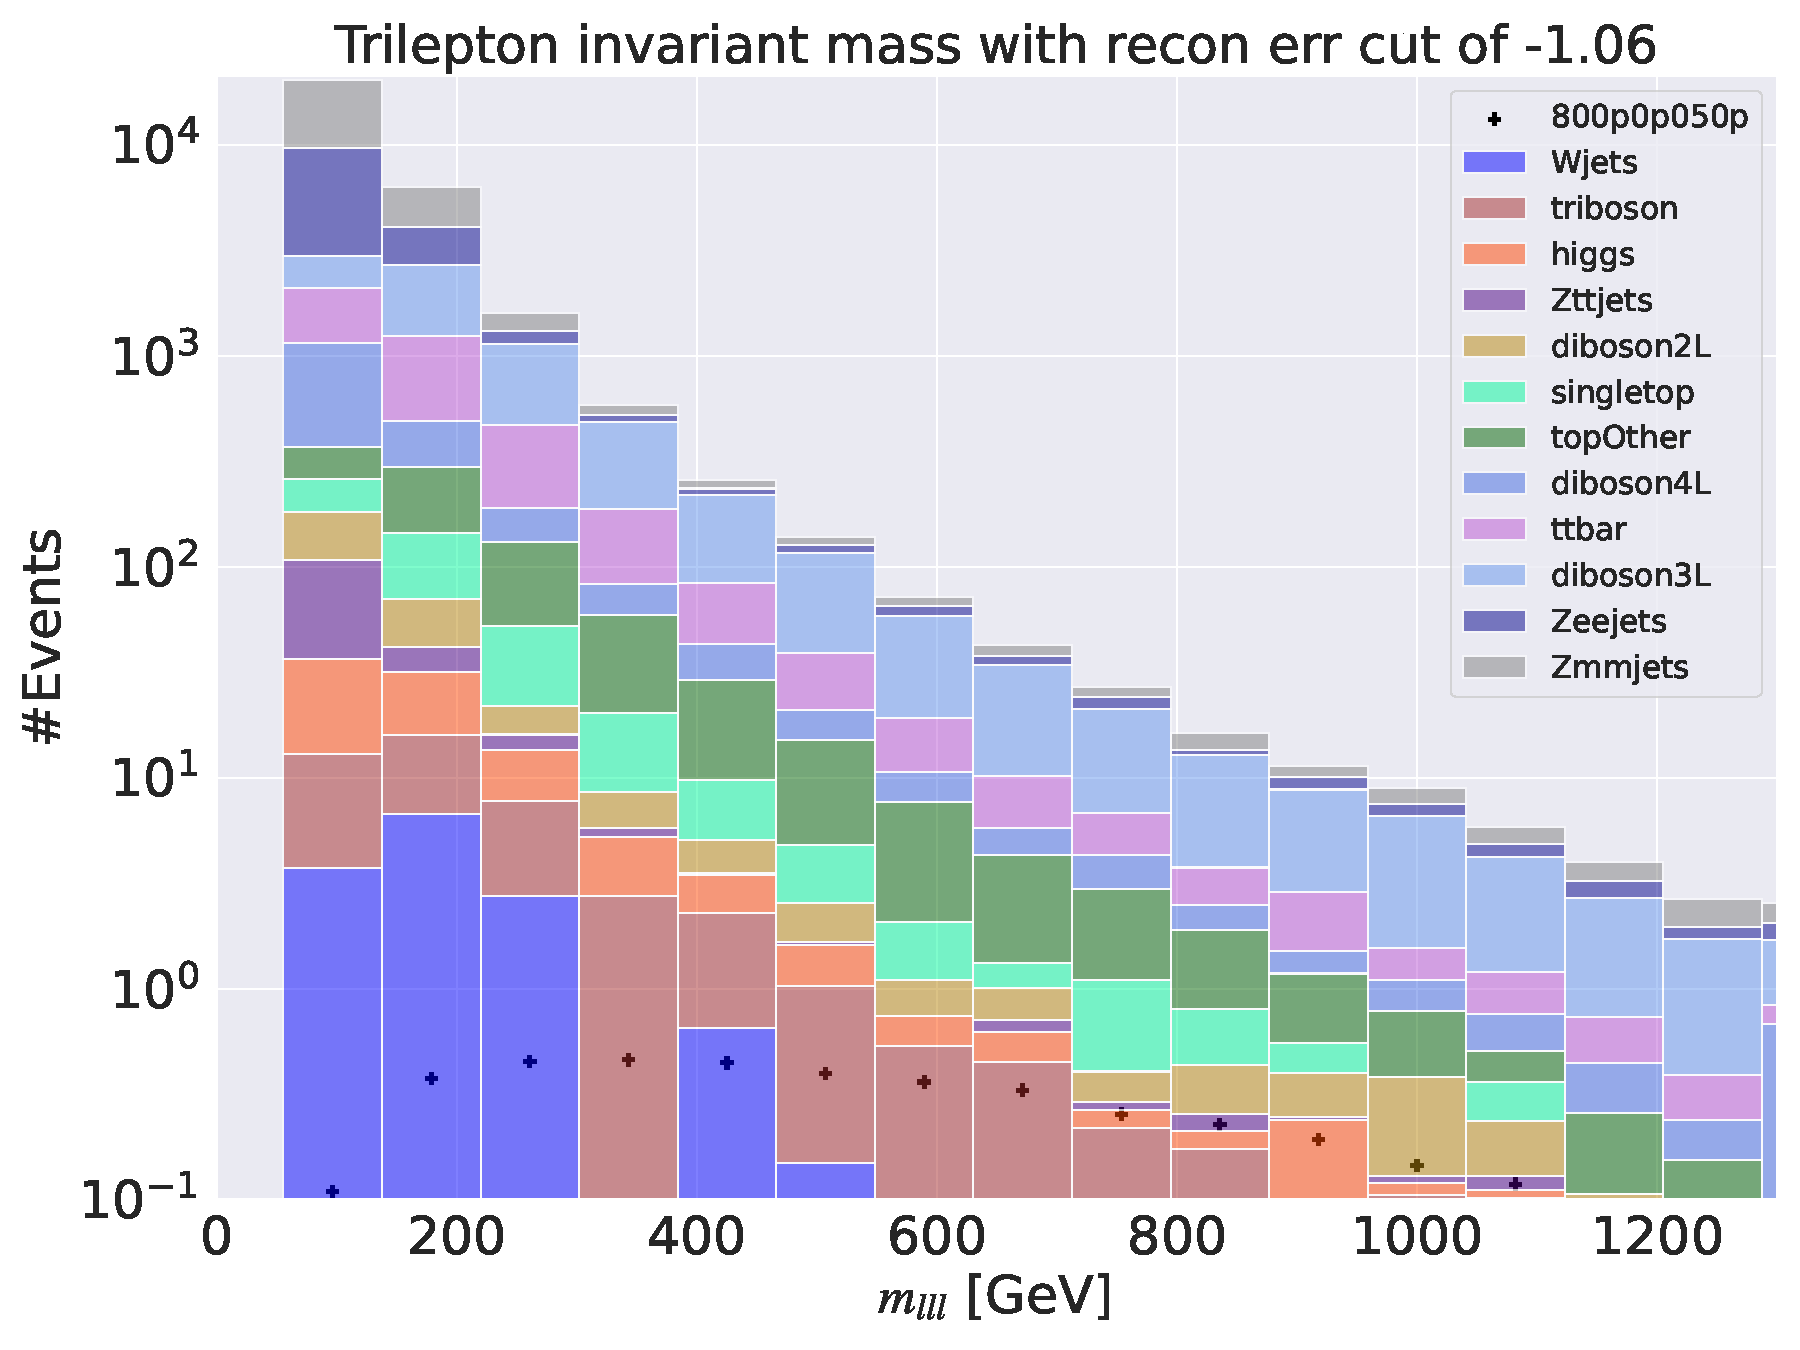
\includegraphics[width=\textwidth]{Figures/VAE_testing/big/3lep/b_data_recon_big_rm3_feats_sig_800p0p050p_mlll_recon_errcut_-1.06.pdf}
        \caption{}
        \label{fig:VAE_3lep_big_mlll_800}
    \end{subfigure}
    \hfill   
    \begin{subfigure}{.49\textwidth}
        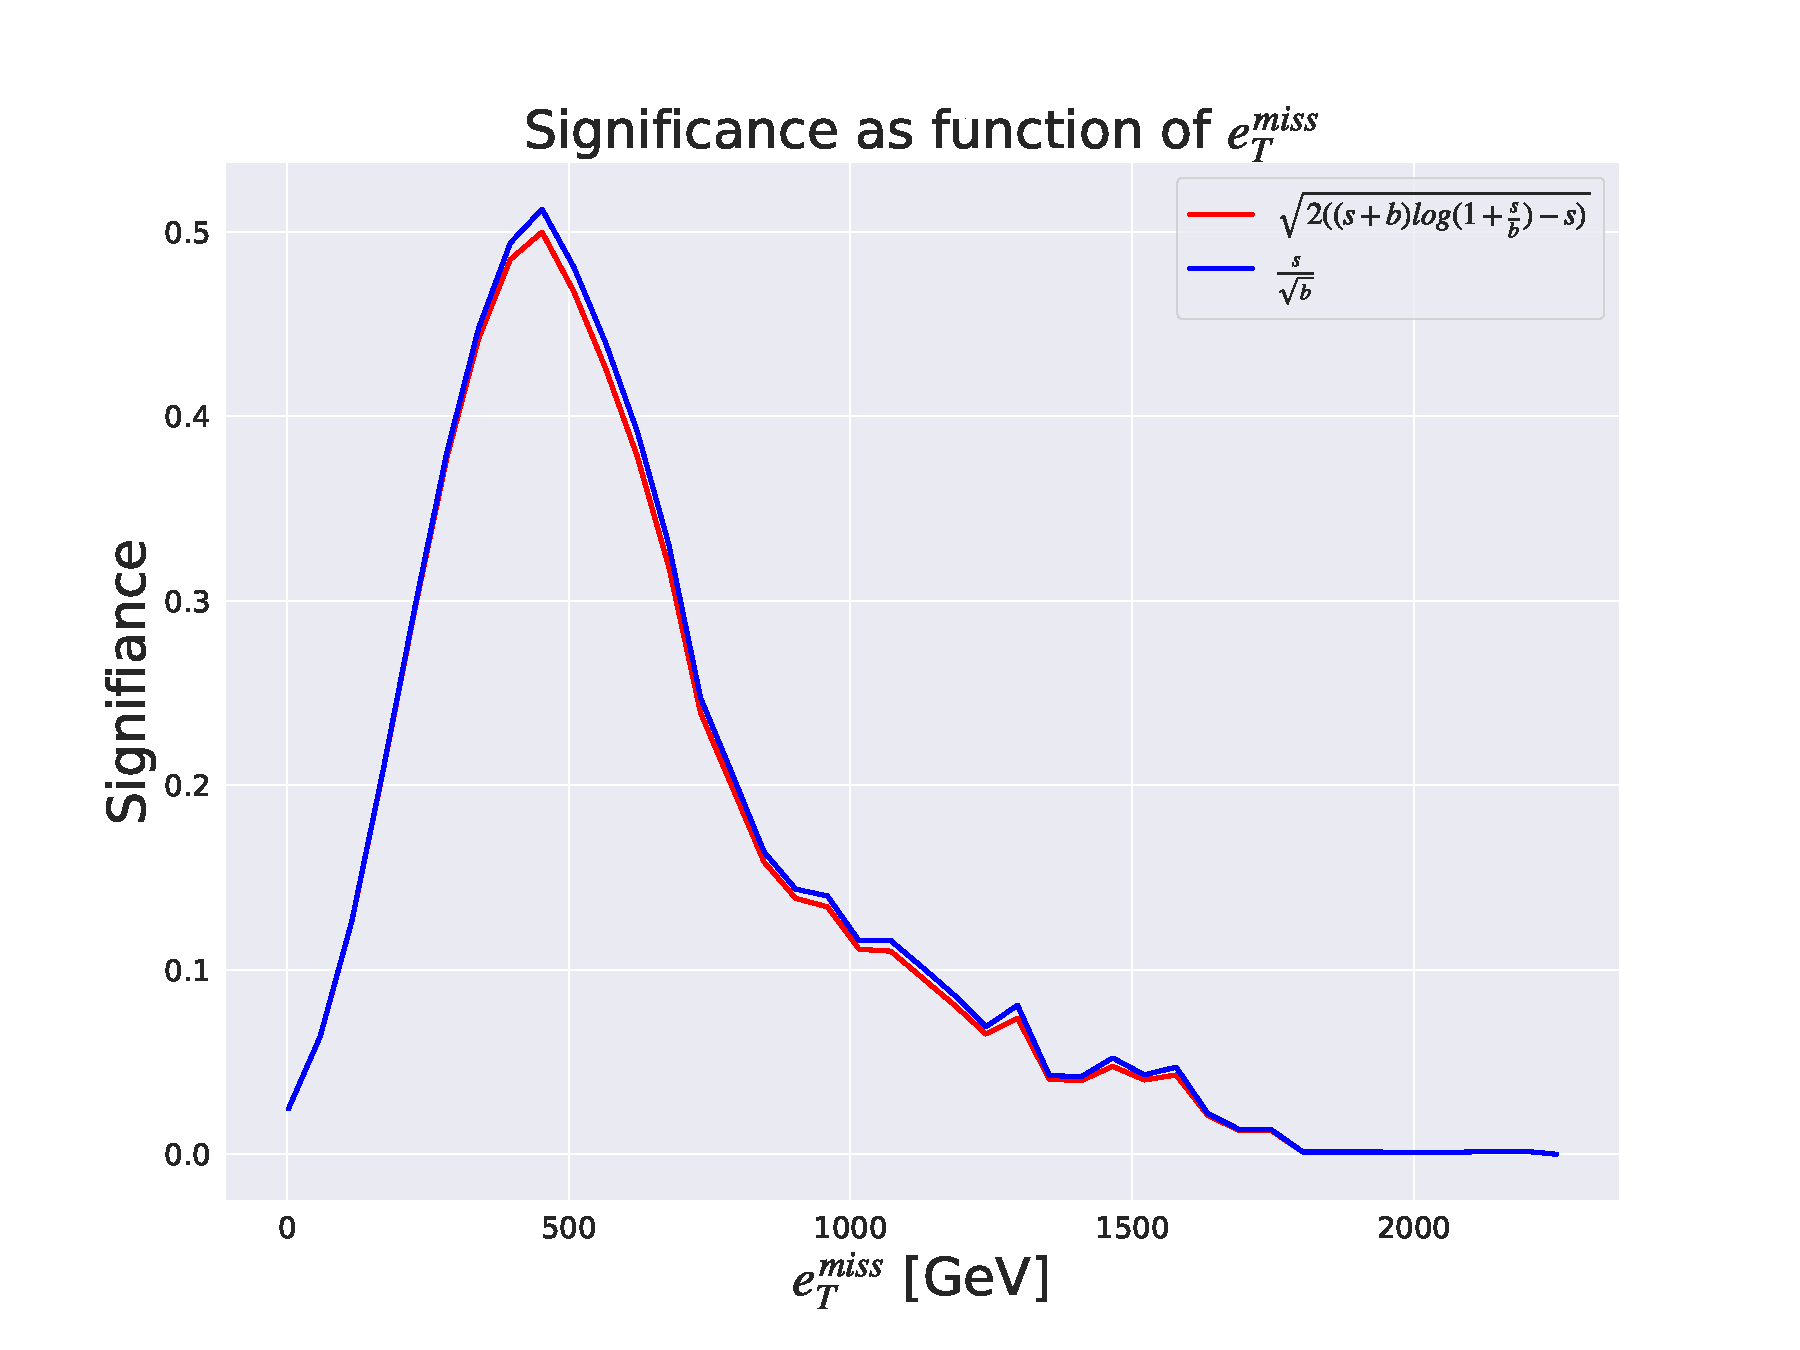
\includegraphics[width=\textwidth]{Figures/VAE_testing/big/3lep/significance_etmiss_800p0p050p_-1.0588523538160817.pdf}
        \caption{}
        \label{fig:VAE_3lep_big_signi_800}
    \end{subfigure}
    \hfill      
    \caption[3lep deep network | $800p50$ | VAE]{Reconstruction error, $e_T^{miss}$ signal region, $m_{lll}$ signal region and significance as function of 
    $e_T^{miss}$ for the deep variational autoencoder using the SUSY $800p50$.
    Figure \ref{fig:VAE_3lep_big_800} shows the reconstruction error 
    distribution for the SM MC and the SUSY signal. Here the autoencoder produces a hill-like for background and 
    signal with little destinction. The peaks of the two distributions are not separated in reconstruction error. Figure \ref{fig:VAE_3lep_big_etmiss_800} 
    shows the $e_T^{miss}$ distribution for the SM MC and the SUSY signal in the signal region. 
    The signal region is made using a cut around $10^{-1.06}$. Some background is removed, and the peaks of the SM MC and signal 
    distributions are separated. Figure \ref{fig:VAE_3lep_big_mlll_800} shows the $m_{lll}$ distribution for the SM MC and the SUSY signal. 
    The shape of both distributions are displaying almost the same shape. Figure \ref{fig:VAE_3lep_big_signi_800} shows the significance as 
    function of $e_T^{miss}$. The peak is put around a cut of about 480 GeV in the $e_T^{miss}$, with a significance of around $0.6$.}
    \label{fig:VAE_3lep_big_rec_sig_signi_800}
\end{figure}

\begin{figure}[h!]
    \centering
    \begin{subfigure}{.49\textwidth}
        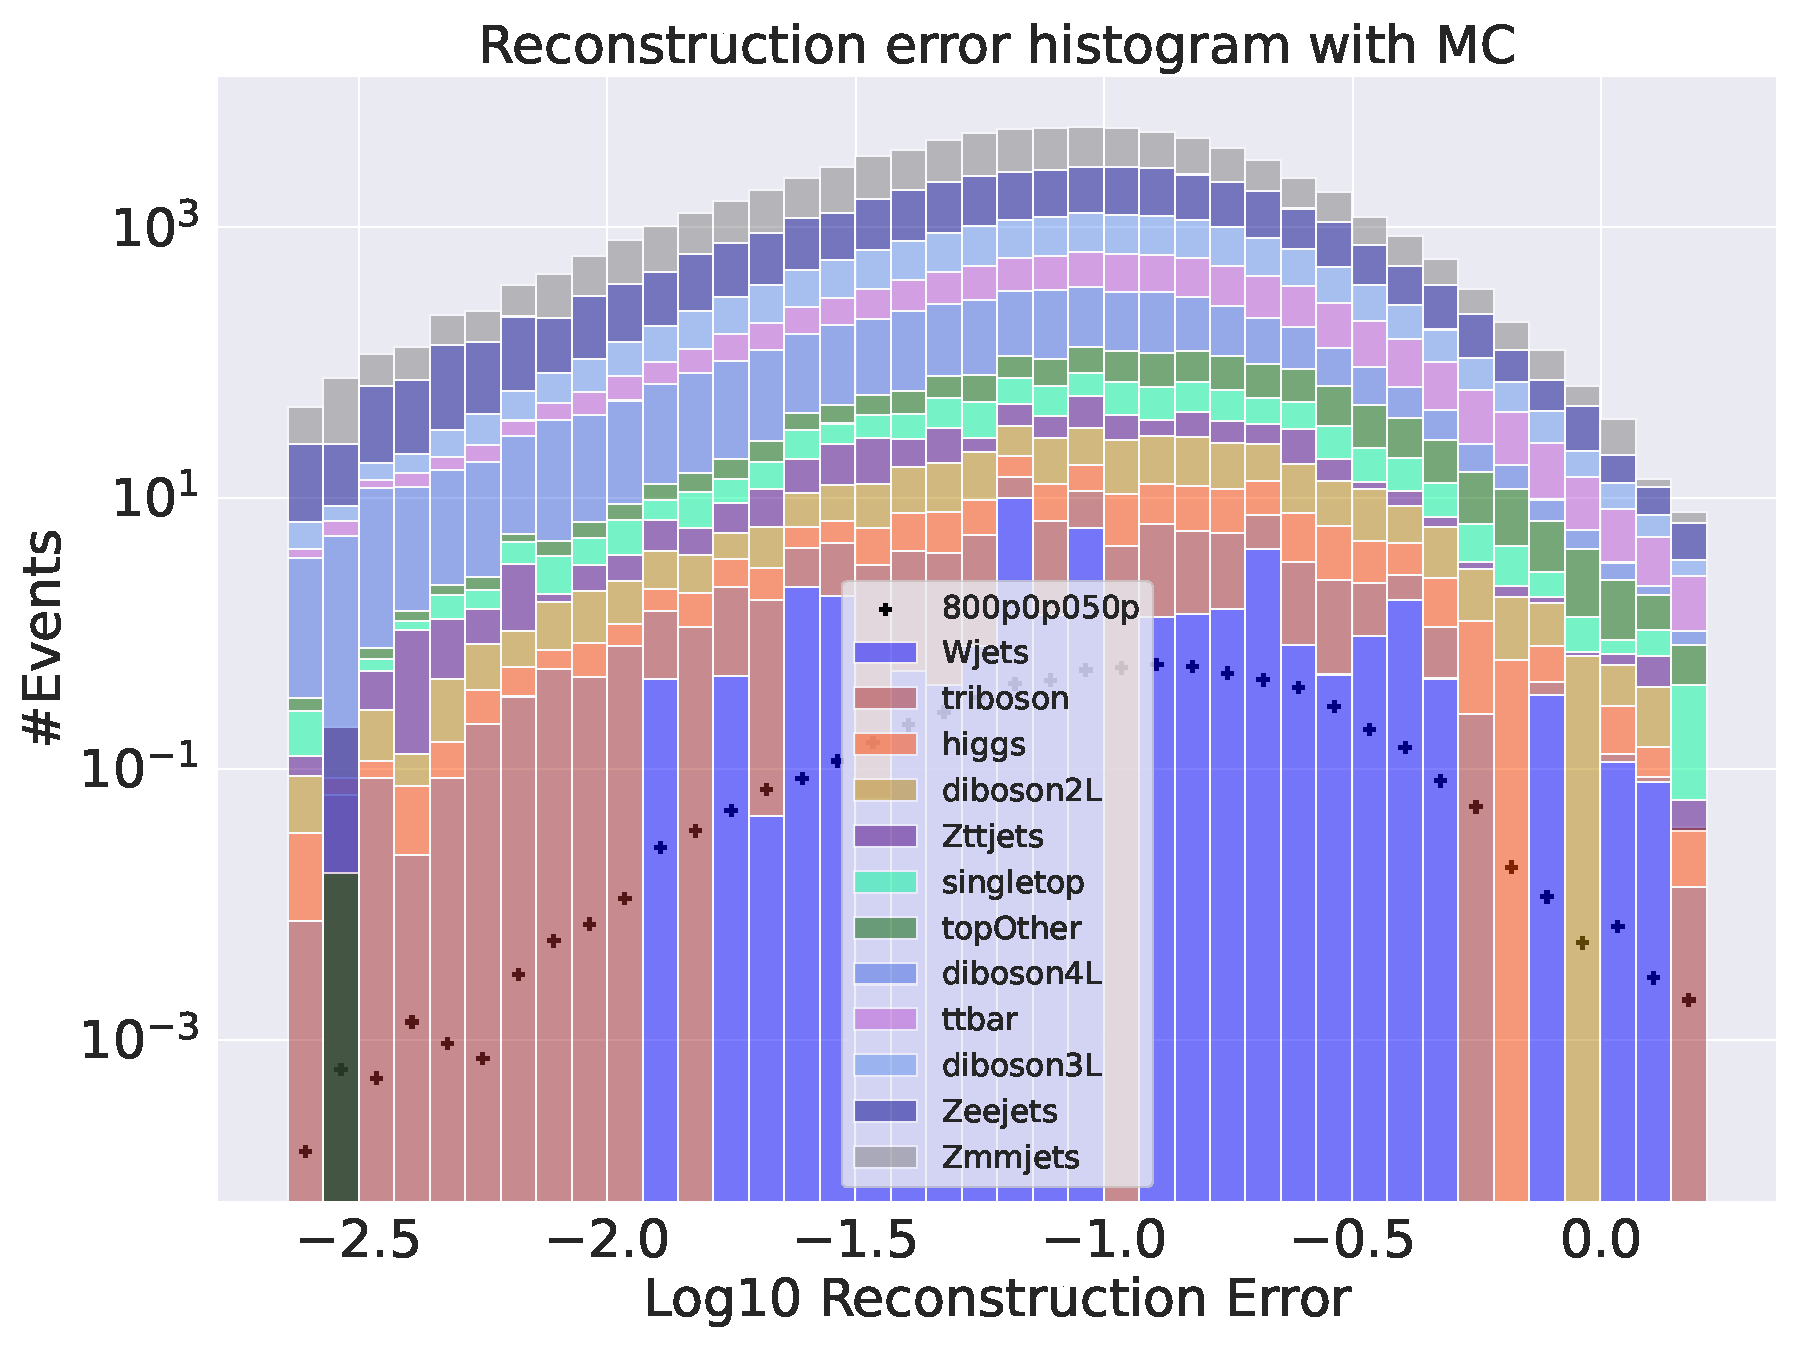
\includegraphics[width=\textwidth]{Figures/VAE_testing/small/3lep/b_data_recon_big_rm3_feats_sig_800p0p050p.pdf}
        \caption{ }
        \label{fig:VAE_3lep_small_800}
    \end{subfigure}
    \hfill
    \begin{subfigure}{.49\textwidth}
        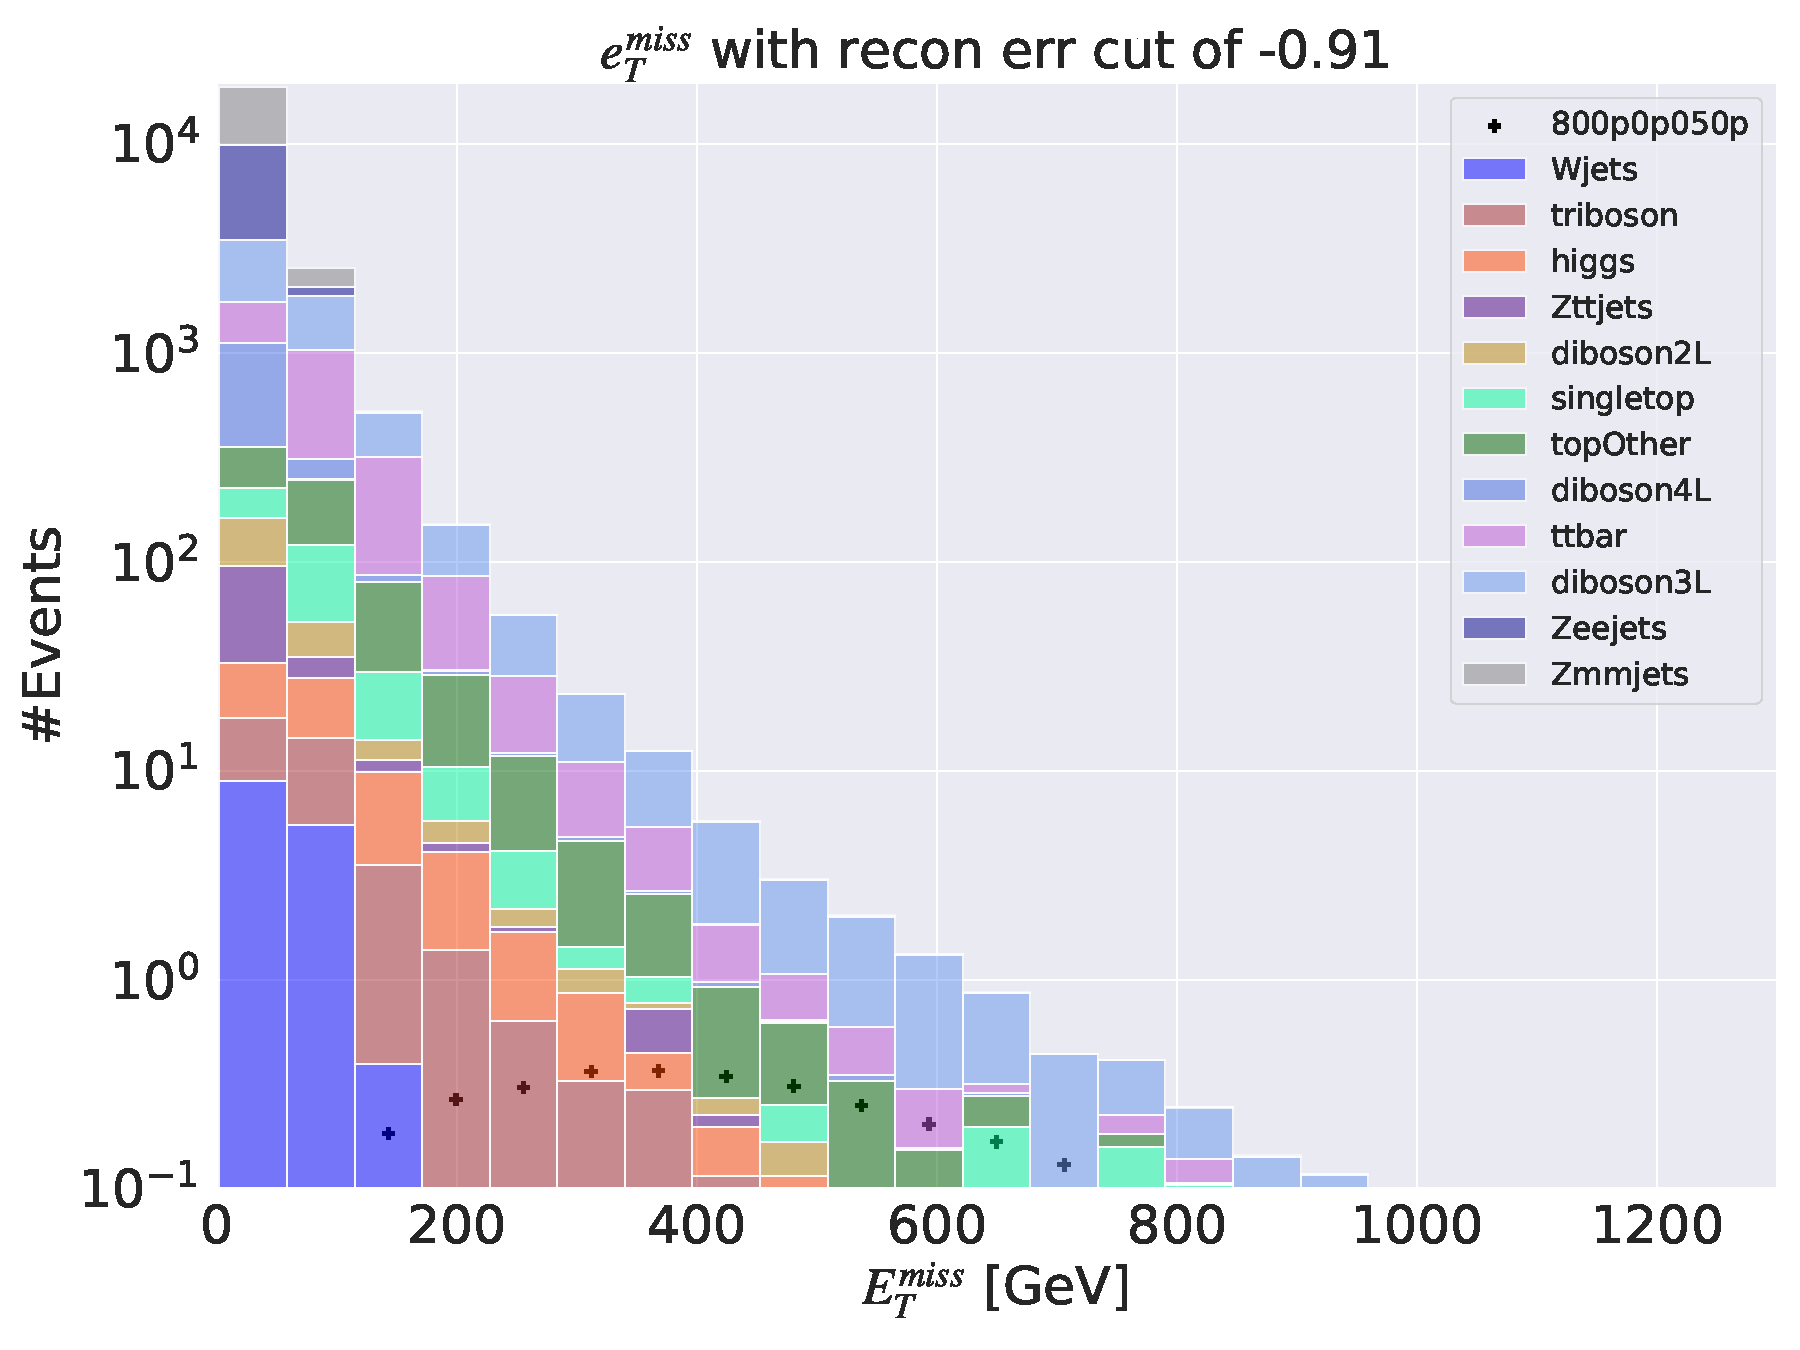
\includegraphics[width=\textwidth]{Figures/VAE_testing/small/3lep/b_data_recon_big_rm3_feats_sig_800p0p050p_etmiss_recon_errcut_-0.91.pdf}
        \caption{}
        \label{fig:VAE_3lep_small_etmiss_800}
    \end{subfigure}
    \hfill
    \begin{subfigure}{.49\textwidth}
        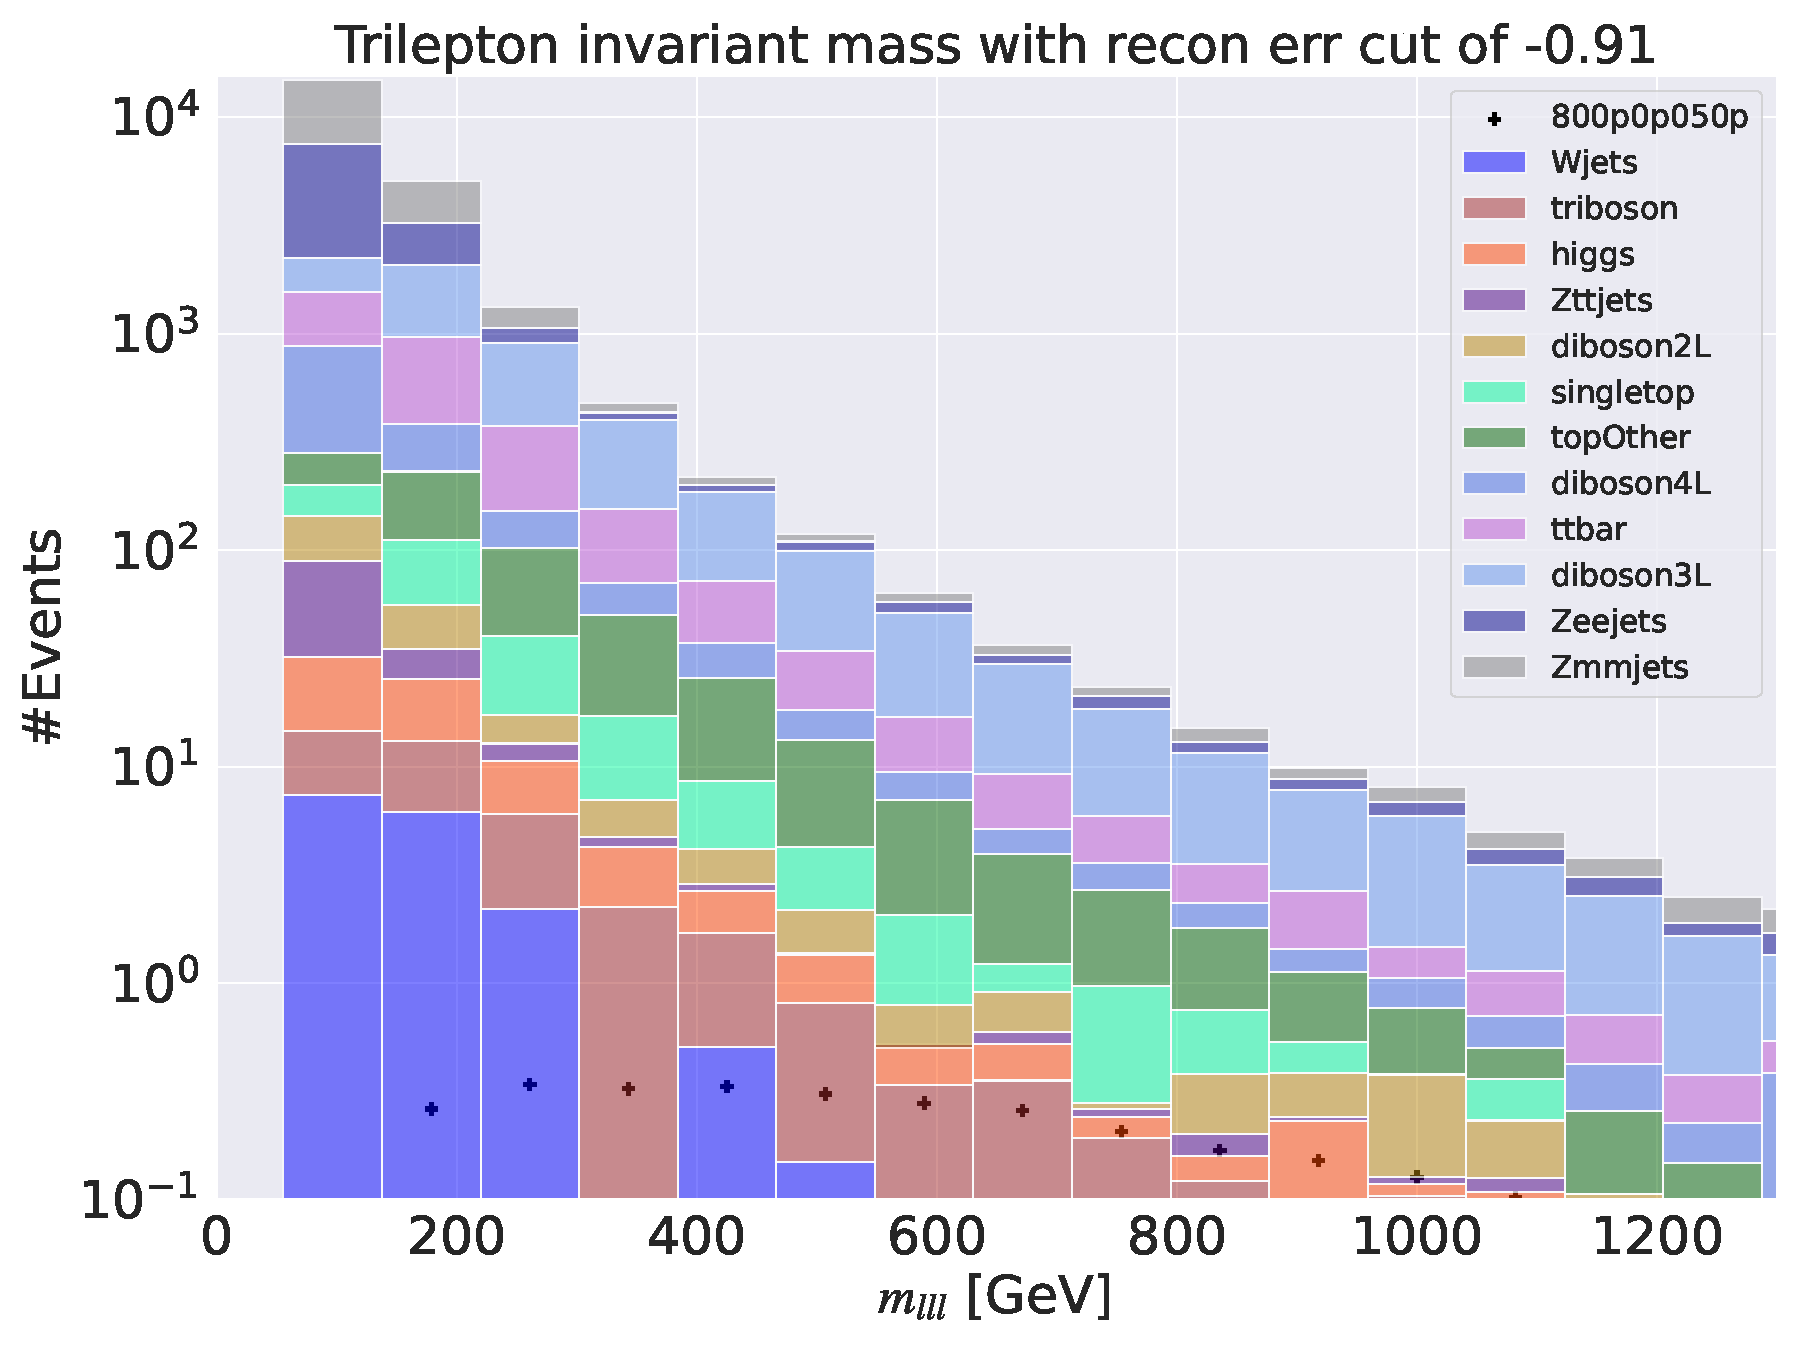
\includegraphics[width=\textwidth]{Figures/VAE_testing/small/3lep/b_data_recon_big_rm3_feats_sig_800p0p050p_mlll_recon_errcut_-0.91.pdf}
        \caption{}
        \label{fig:VAE_3lep_small_mlll_800}
    \end{subfigure}
    \hfill   
    \begin{subfigure}{.49\textwidth}
        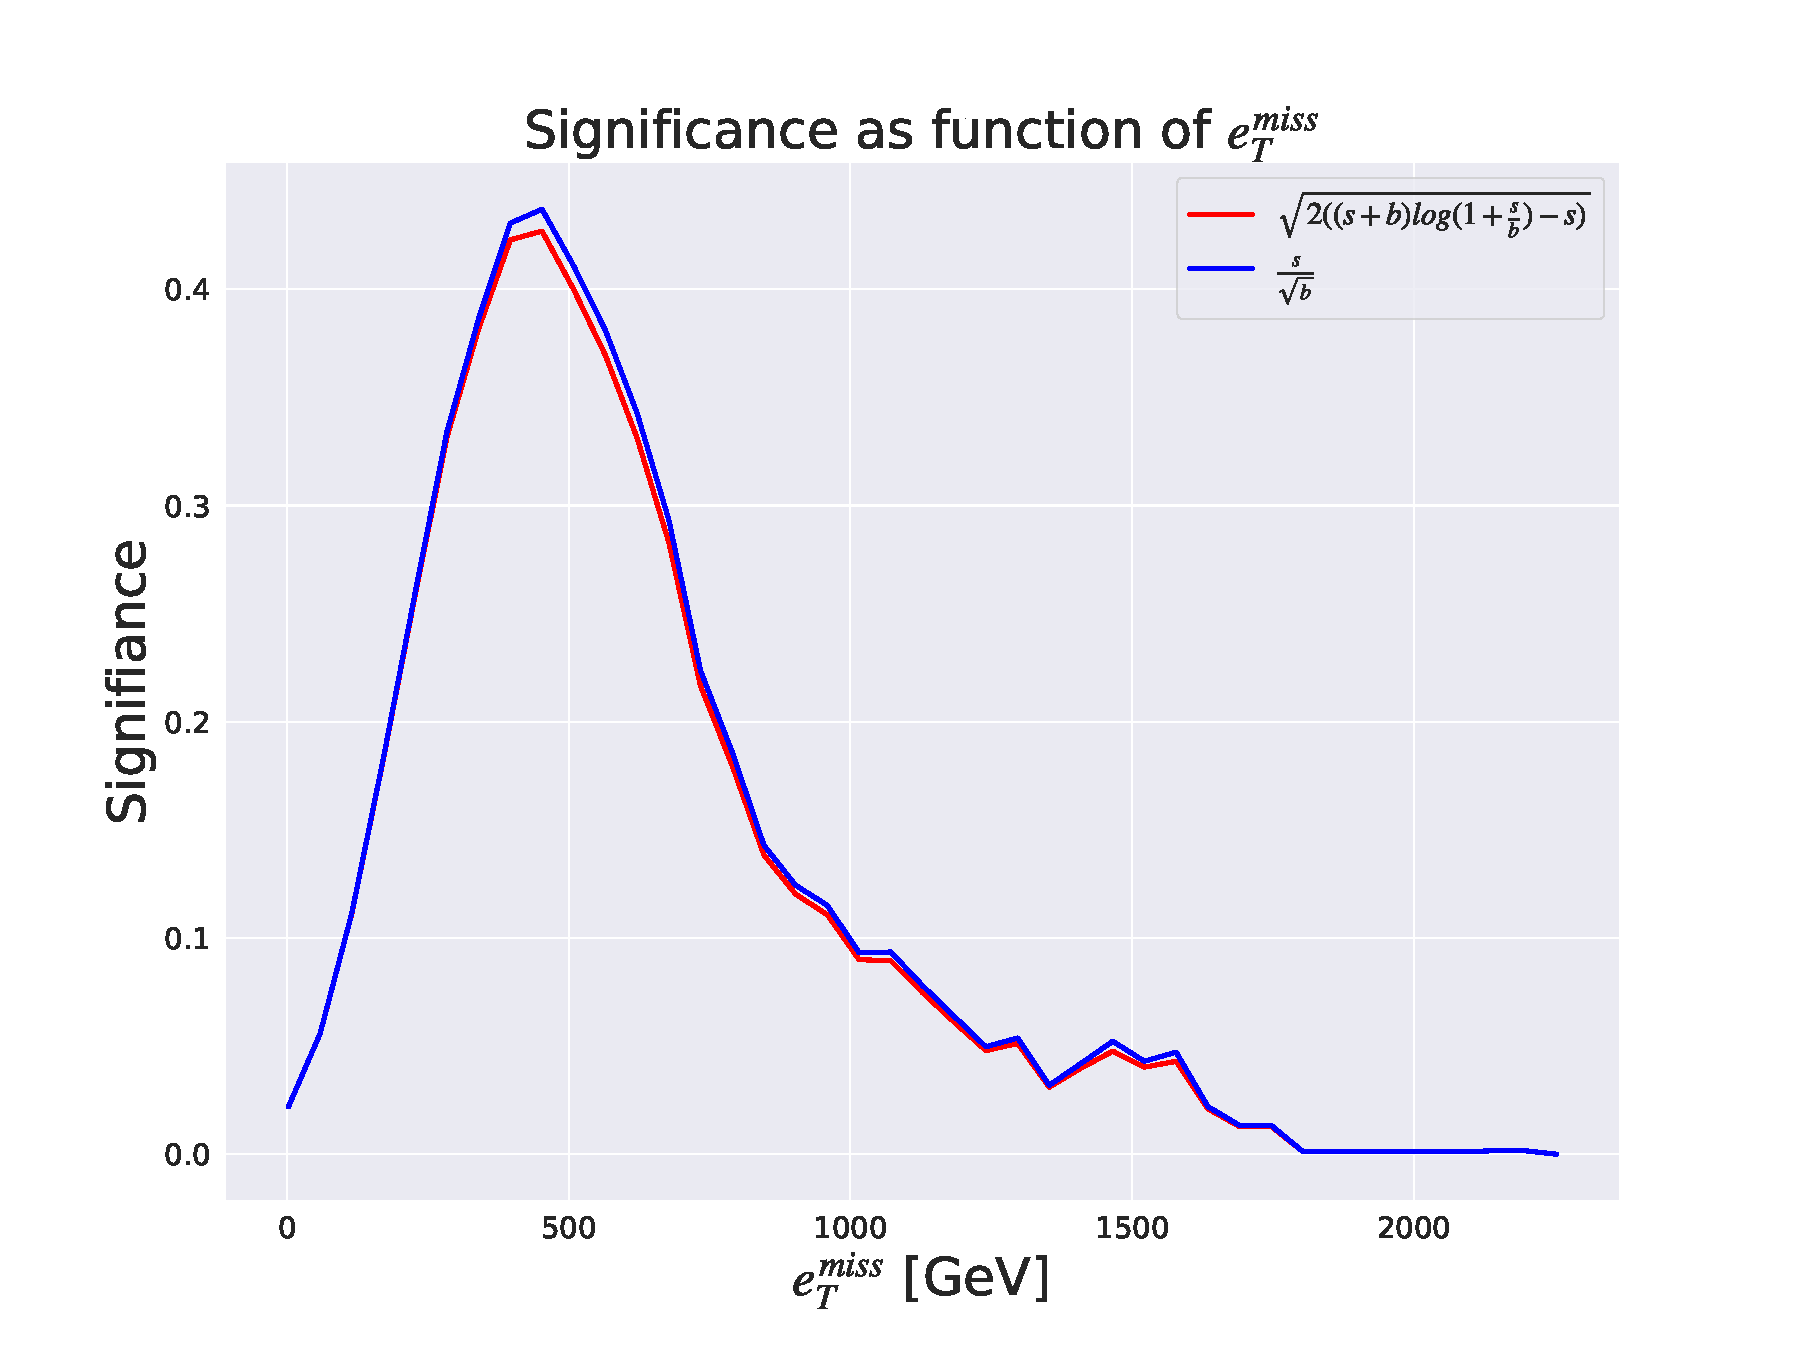
\includegraphics[width=\textwidth]{Figures/VAE_testing/small/3lep/significance_etmiss_800p0p050p_-0.9142561918890106.pdf}
        \caption{}
        \label{fig:VAE_3lep_small_signi_800}
    \end{subfigure}
    \hfill      
    \caption[3lep shallow network | $800p50$ | VAE]{Reconstruction error, $e_T^{miss}$ signal region, $m_{lll}$ signal region and significance as function of 
    $e_T^{miss}$ for the shallow variational autoencoder using the SUSY $800p50$.
    Figure \ref{fig:VAE_3lep_small_800} shows the reconstruction error 
    distribution for the SM MC and the SUSY signal. Here the autoencoder produces a hill-like for background and 
    signal with little destinction. The peaks of the two distributions are not separated in reconstruction error. Figure \ref{fig:VAE_3lep_small_etmiss_800} 
    shows the $e_T^{miss}$ distribution for the SM MC and the SUSY signal in the signal region. 
    The signal region is made using a cut around $10^{-0.91}$. Some background is removed, and the peaks of the SM MC and signal 
    distributions are separated. Figure \ref{fig:VAE_3lep_small_mlll_800} shows the $m_{lll}$ distribution for the SM MC and the SUSY signal. 
    The shape of both distributions are displaying almost the same shape. Figure \ref{fig:VAE_3lep_small_signi_800} shows the significance as 
    function of $e_T^{miss}$. The peak is put around a cut of about 480 GeV in the $e_T^{miss}$, with a significance of around $0.45$.}
    \label{fig:VAE_3lep_small_rec_sig_signi_800}
\end{figure}


Figures \ref{fig:VAE_3lep_big_rec_sig_signi_450}, \ref{fig:VAE_3lep_small_rec_sig_signi_450}, 
\ref{fig:VAE_3lep_big_rec_sig_signi_800} and \ref{fig:VAE_3lep_small_rec_sig_signi_800} contain four 
subplots with the total reconstruction error distributions (a), the $e_T^{miss}$ signal region (b), 
the $m_{lll}$ signal region (c) and the significance as function of $e_T^{miss}$ curve (d) respectively 
for the shallow and deep variational autoencoder. From figures \ref{fig:VAE_3lep_big_450}, \ref{fig:VAE_3lep_small_450},
\ref{fig:VAE_3lep_big_800} and \ref{fig:VAE_3lep_small_800} we observe that the variational 
autoencoder seems to struggle with differentiating between background and signal. 
There is however a slight difference in the shape of the distributions from the shallow and 
deep network shown in both signal test cases. The shallow has a more narrow and slightly more 
left-skewed shape, whereas the deep network has a slightly more broad distribution shifted a 
bit to the right. The bulk of the events for all four histograms are between $10^{-2}$ and $10^{-0.5}$ 
reconstruction error, indicating that the autoencoder struggles to learn the internal RMM 
structures for the 3 lepton + $e_T^{miss}$ final state MC. \par 
In figures \ref{fig:VAE_3lep_big_etmiss_450}, \ref{fig:VAE_3lep_small_etmiss_450}, 
\ref{fig:VAE_3lep_big_etmiss_800} and  \ref{fig:VAE_3lep_small_etmiss_800} we have the 
reconstruction error cut imposed on the SM MC and the signal samples. Interestingly, one should 
note that although the total reconstruction error distributions are not well separated, the 
signal regions show a separation in the $e_T^{miss}$ distribution. Unlike in the regular autoencoder 
case, the variational autoencoder allows for almost two orders of magnitude more background 
events in the signal region. This is because of the signal region definition from section 
\ref{sec:strategy} where the median for all four cases with the variational autoencoder is where in the peak of the 
reconstruction error distribution for the background. Therefor we also get the peak of 
the signal distributions, which is why we see so much signal in the signal region in figures 
\ref{fig:VAE_3lep_big_etmiss_450}, \ref{fig:VAE_3lep_small_etmiss_450}, 
\ref{fig:VAE_3lep_big_etmiss_800} and \ref{fig:VAE_3lep_small_etmiss_800}. \par 
In figures \ref{fig:VAE_3lep_big_mlll_450}, \ref{fig:VAE_3lep_small_mlll_450}, 
\ref{fig:VAE_3lep_big_mlll_800} and  \ref{fig:VAE_3lep_small_mlll_800} we have the signal 
region in the $m_{lll}$ feature. Here, as with the $e_T^{miss}$ distribution, the least 
strict reconstruction error cut has been imposed on the region. It is shown that the 
difference between the shallow and deep neural network architecture has little to no effect 
here or in the $e_T^{miss}$ distributions in terms of separation. \par 
In figures \ref{fig:VAE_3lep_big_signi_450}, \ref{fig:VAE_3lep_small_signi_450}, \ref{fig:VAE_3lep_big_signi_800} and  
\ref{fig:VAE_3lep_small_signi_800} we have the significance as a function of the $e_T^{miss}$.
Interestingly, for the SUSY $450p300$ case, we have that both the deep and shallow 
autoencoder manages to get a significance of around 4, which is much better than the 
regular autoencoder which got around 0.7. For the SUSY $800p50$ signal the difference between the significance 
from the AE and VAE was small. From these figures a further cut on the 
$e_T^{miss}$ on around 400 GeV provided the best significance of around $4.5$. 
